\chapter{Introduction}
\label{introduction}

 \begin{quote} 

All forms of communication entail design, as the intent of communication is to be understood by others or by one's self at another time. Communication design, then, is inherently social, because to be understood by another or by self at another time entails fashioning communications to fit the presumed mental states of others or of one's self at another time.  \citep[p. 6]{Tversky:2010ww} 
 \end{quote} 

\section{Mis-Communication in Interaction Design}
\label{mis-communicationininteractiondesign}

Good interaction design takes into account user cognitive processes and limitations. Though designers spend considerable effort toward producing user interfaces and interactions that communicate effectively, the tools that they use are flexible can easily bend to cause users to make incorrect inferences about the situation at hand. Because graphical users interfaces (GUIs) share properties with other forms of communication such as language, gesture, diagrams and action --- and are inherently interactional --- \emph{I argue that they are also subject to the same context-dependent aspects of meaning that arise with language use}. The same cognitive architecture that supports understanding of language also supports and facilitates understanding of user interfaces. This observation forms the basis for claims made in this dissertation.

In traditional GUI-based interaction, user interactions are designed. When a user interacts with a website, that interaction is structured according to that site designer's plan. Ideally, information has been organized with user expectation in mind. The designer has considered the sorts of tasks users intend to perform. Sometimes, navigation is guided. Sometimes not, but designers leave behind contextual cues and guideposts to aid users in their task.

In fact, it is easy to influence users to act in predictable ways. For example,  \cite{Tversky:1981vc}  showed that predictable, dramatic shifts in preference could be generated simply by changing the ways options are framed: in early framing experiments, subjects showed a preference toward risk aversion when lotteries were framed as gains, and risk seeking when lotteries were framed as losses. 

As noted by  \cite*{Thaler:2010uy},  designers have the potential for great control over user decision-making by manipulating behavior using psychological tools described by psychologists and behavioral economists. However, though  \cite{Kahneman:1984td}  and others have noted that small changes in context affects decision-making, there is considerably less research on how \emph{small changes in context affect understanding in the context of decision-making}.

Language operates using the same principles and processes as other cognitive functions. It is not surprising to learn that language can be used to manipulate hearer understanding. For example,
 
\begin{enumerate} 
\item[(1)] The Sheriff caught Robin red-handed. He is now serving time in prison.
\end{enumerate}

Sentence 1 above appears to convey the following facts that weren't explicitly stated:

\begin{enumerate} 
\item[(1a)] It is Robin who is serving time in prison.
\item[(1b)] Robin is serving time in prison as a result of being caught red-handed by the Sheriff.
\end{enumerate}

These un-stated propositions (1a) and (1b) are known as \emph{implicatures}, a well-known pragmatic phenomenon in language understanding. In fact, depending on situational context, either of these implicatures may not be  true.\footnote{Imagine you are watching a humorous movie and (1) is a caption. The Sheriff caught Robin Hood returning illegal taxes back to the citizenry. Later, the Sheriff was jailed for fraud. Though we might ordinarily expect the second sentence in this example to have a causal relation to the first, the visual scene serves as a contextual backdrop cancelling the implicature.}  Implicatures operate under principles such that we may presume their truth even if un-stated. But if the truth value of either implicature (1a) or (1b) turns out to be false, this does not mean that (1) is false.

Because what we know is so often derived by inference, it is easy to see how language can be used to manipulate understanding. But is it possible for GUIs to communicate in the same sort of way? I believe so. This dissertation will show that GUI-based mis-communications may be brought about by faulty inferences.

\section{Discourse Understanding}
\label{discourseunderstanding}

Discourse is generally said to encompass language use beyond the bounds of a sentence or proposition. It is often associated with the study of pragmatics: ``Syntax studies sentence. Semantics studies propositions. Pragmatics is the study of linguistic acts and the contexts in which they are performed''  \citep[p. 34]{Stalnaker:1999vl}.  Pragmatics attempt to account for meaning of messages where actual meaning is underdetermined from what is said. 

Pragmatics is fundamentally concerned with reasoning processes that go beyond conventional meaning to interpretation in social, situational, and belief contexts. As such, it is founded on the notion of language as action with communicative goals  \citep{Grice:1975vz,Levinson:2000ud,Clark:1996tm}.  In this view, ``hearers'' infer a ``speaker's'' meaning on the basis of evidence provided.

\begin{sloppier}
Discourse is also studied by sociologists, anthropologists, and sociolinguists: it is bound to socio-cultural knowledge and governed by social norms \citep{Gumperz:1982tc,Hymes:1974wr}.  Even so, discourse communication is seen as structured: both in terms of conversational events and learned, ritualistic schemas \citep[e.g., making a reservation]{Goffman:1981tm}. In this tradition, conversational inferences are also context-bound, but conceived more generally as preferences, maxims, or tendencies.
\end{sloppier}


\section{Confusion in Online Behavioral Advertising}
\label{confusioninonlinebehavioraladvertising}

Of concern to nearly everyone on the Internet today is privacy. Polls conducted over the last decade indicate that the majority of Internet users report that they do not wish to be tracked across sites  \citep{Truste:2012uc}.  At the same time, Internet advertising has entered a boom for mass data collection and predictive analytics. While it may be in the best interest of consumers to restrict online data collection and tracking, in practice, the legal system has been unable to keep pace. Even so, businesses that engage in online behavioral advertising (OBA) commonly employ techniques that influence user behavior by manipulation. The goal of advertisers, after all, is to influence consumers and sell products. 

Pertaining to OBA, the following sorts of questions are addressed in this dissertation:

\begin{itemize}
\item Why might users say privacy is important but not choose to block cookies when given a choice?

\item Why is the Interactive Advertising Bureau (IAB) AdChoices opt-out icon confusing to so many users?

\item Why might might users, who acknowledge that the Internet is not private, behave as if it is?
Such questions relate to user belief and decision-making in the context of website interactions on the Internet.

\end{itemize}

Though advertising language has been studied in the \emph{content} of ads  \citep{Leech:1966wr,Geis:1982uf,Harris:1983tj,Vestergaard:1985vn,Cook:2001up,Tanaka:1999tq},  the study of how advertisers might influence users during the course interaction has not yet been addressed. 

\section{Empirical Study}
\label{empiricalstudy}

In this dissertation, I use randomized controlled experimentation to observe user behavior under specific conditions. Each experiment asks: is there mis-understanding and is such confusion pragmatic in nature?

The first experiment hypothesizes the interpretation of \textbf{implicature} in ``do not track'' dialog boxes. Such dialog boxes are often presented as modal dialogs, thus, as an unforced ``yes-no'' choice design. In experiment 1A, I examine whether graphical representations of choice in this context evoke implicature in the same manner as textual representations. Following this, experiment 1B considers what people believe is the consequence of ``no choice'' in task-based interaction.

The second experiment focuses on the role of \textbf{deixis} in hyper-linked ad images. The Interactive Advertising Bureau (IAB) AdChoices icon associated with behavioral advertisements is designed to give users the means to control behavioral tracking preferences. However, relatively few people notice such  icons,\footnote{This is based on a national wireline and cell telephone survey of 1,503 adult Americans during April and May, 2012 \citep{TheNonTransparency:2012ut}.}  let alone click them  \citep*{TheNonTransparency:2012ut,Logic:2011wn}.   \cite*{Leon:2012dk,Ur:2012ws}  describe communicative flaws with AdChoices icon. While they considered the effect of iconic versus textual communication, they only speculate on causes for confusion. Experiment 2A hypothesizes that knowledge plays a role in whether an icon is taken to be indexically linked to a website. Experiment 2B considers whether familiar iconic representations affect how users interact with advertisements in context.

Finally, Experiment 3 focuses on the pervasive phenomenon of third-party tracking in the browser itself. In this study, user interaction on the Internet is analyzed as a form of multi-party discourse leading to to issues in \textbf{conversational inference} where the user does not infer the presence of unratified participants monitoring web interactions. Manipulating the user's perceptual awareness of third party participants is hypothesized to have an effect on user behavior. More broadly, this experiment attempts to show that user behavior, while answering sensitive questions, is affected in the presence of visible observers. I hypothesize that their propensity for disclosure of sensitive information is reduced under such conditions.

In each experiment described above, I show how advertisers may either benefit from poor design decisions or deliberately mis-lead users through the manipulation of linguistic understanding. Though the context for experimentation is situated in the domain of online behavioral advertising, the method for analysis is general in nature. 

\section{Thesis Aim}
\label{thesisaim}

The aim of this thesis is to prove that certain problems and confusions that users face interacting with technology associated with online behavioral advertising can best be understood as problems in discourse understanding. Using quantitative methods, I demonstrate that users are subject to the same context-dependent aspects of meaning that arise with the use of language. With the rise of new interactions fueled by behavioral advertising, I argue that advertisers may look toward exploiting new opportunities for manipulating meaning and understanding.

This thesis does not intend to catalog the full range of discourse phenomena extant in user interaction --- nor does it attempt to solve the problems described. It also doesn't intend to cover the entire range of phenomena within the context of OBA. The intent is to reveal how a linguistic analysis may account for user confusion not fully explained otherwise. Such confusions emphasize the need for designers to consider the importance of discourse inference in GUI-based interaction.

Chapter 2 introduces background literature on the topic of online behavioral advertising This chapter lays the foundation for analyzing observed phenomena under an inferential model of communication. Chapter 3 describes the discourse-theoretic framework necessary for testing hypotheses about pragmatic processes. Chapter 4 details a general method for study. Chapters 5, 6, and 7 each describes an experiment addressing a particular problem. Chapter 5 is concerned with whether implicature can be observed in choice processes via a non-forced choice modal dialog interaction. Chapter 6 considers knowledge and the role of deixis in hyperlinked ads. And Chapter 7 highlights the role of conversational inference in an experiment designed to ascertain whether user behavior changes in the presence of observers. Finally, Chapter 8 presents a discussion of results and offers direction for future research. It is my belief that this thesis lends deeper insight into communicative challenges for user interaction design and bridges these to sound theoretical tools for addressing a specific class of problems previously unidentified.

\chapter{Online Behavioral Advertising}
\label{onlinebehavioraladvertising}

This chapter provides an introduction to the concept of online behavioral advertising (OBA). This domain is the backdrop against which experimental hypotheses in this dissertation are tested. Since I began writing this dissertation, OBA has grown from relative obscurity to notoriety. With the rising prominence of mobile browsing, cookie tracking is predicted to disappear within a few years. The surge of public awareness of OBA has recently led to new default settings in some browsers where third-party cookies are blocked by  default.\footnote{Mozilla and Microsoft have moved to this in the past year, while Apple Safari has blocked cookies by default for some time. Meanwhile, Microsoft, Google, and Apple are all exploring new technologies amenable to tracking across platforms to include mobile, gaming, and video services \citep{DOrazio:2013tx}.}  Though particular issues discussed in this chapter will quickly stale, research in this dissertation should not as it relies upon theoretical tools and methods generalizing to phenomena not yet observed. 

This chapter is organized in the following way. First I discuss the phenomenon of OBA and circumstances that led to its meteoric rise. Second, I introduce privacy issues in terms of how data is collected and used by third party advertisers. This has played an important role in shaping policy, leading to the design of interactions examined in this dissertation. Therefore, I follow by outlining the scope of user confusion as observed by privacy researchers. Finally, I conclude by summarizing the sorts of interactions behavioral advertising has engendered and speculate on what we may see in the future. Advertising is becoming increasingly becoming less of a broadcast art and more a personalized one. For this reason, we need to take a closer look at how advertisers may manipulate our thinking and beliefs during the course of interaction.

\section{Intimate Capital}
\label{intimatecapital}

A new market-driven ecosystem of targeted advertising has emerged, spanning the divide of Internet and brick-and-mortar business. This ecosystem is fueled by the unprecedented availability of data, algorithms, storage, and computing power. The forbidden fruit, and yet golden chalice, is the ability for the advertiser to know the target intimately. Of serious concern outside the advertising industry is that behavioral data may be combined with data owned by other content publishers or advertisers to actually identify a particular user. The more an advertiser knows the user --- and not just as a demographic profile but as an individual --- the more fine-grained the targeting. So it would not be surprising to learn that publishers and advertisers treat information about consumers as a form of capital --- an ``intimate capital{\ldots} likely to be worth something to others''  \citep[p. 127]{Locke:2010wt}.  This section focuses on the sorts of data advertisers track and how this data is used in behavioral advertising. The availability of such data, coupled with advances in computing technology have given rise to new market economies struggling to maximize a return-on-investment (ROI) while the very measures defining ROI and ad effectiveness are in flux.

\subsection{Science in Advertising}
\label{scienceinadvertising}

The quote below from a 1901 article in Publicity seems almost prescient by today's standards:


\begin{quote}
The time is not far away when the advertising writer will find out the inestimable benefits of a knowledge of psychology. The preparation of copy has usually followed the instincts rather than the analytical functions. An advertisement has been written to describe the articles which it was wished to place before the reader; a bit of cleverness, an attractive cut, or some other catchy device has been used, with the hope that the hit or miss ratio could be made as favorable as possible. But the future must needs be full of better methods than these to make advertising advance with the same rapidity as it has during the latter part of the last century. And this will come through a closer knowledge of the psychological composition of the mind. The so-called 'students of human nature' will then be called successful psychologists, and the successful advertisers will be likewise termed psychological advertisers. The mere mention of psychological terms, habit, self, conception, discrimination, association, memory, imagination and perception, reason, emotion, instinct and will, should create a flood of new thought that should appeal to every advanced consumer of advertising space \citep[as cited in][]{Scott:1904td}.
\end{quote}


That these concepts should transfer so easily to the  21\textsuperscript{st}  century Internet is startling: what held true in advertising more than 100 years ago still rings true today.

In 1957, when Vance Packard wrote the runaway best seller The Hidden Persuaders, he exposed advertising not as a huckster bag of tricks, but as a subtle and calculated science with deep roots in psychoanalysis, sociology, and ethnographic anthropology. He honed in on a group of psychologists known as ``the depth boys'' who believed that to understand the consumer, you needed to find out what they really wanted at an unconscious level. In previous decades, advertisers had found little success interviewing and asking people what they wanted in a product. From \emph{Advertising Age}, ``In very few instance do people really know what they want, even when they say the do''  \citep[as cited in][p. 37]{Packard:1957vs}.  According to Packard, what marketers and psychologists had been learning is that what people tell interviewers has little bearing on how they would actually behave. ``What you are more likely to get, they decided, are answers that will protect the informants in their steadfast endeavor to appear to the world as really sensible, intelligent, rational beings''  \citep[p. 35]{Packard:1957vs}.  What advertisers ultimately learned from motivational research was how to find psychological and emotional levers that would generate an affinity to a particular product over a myriad of close alternatives --- and how to use those levers to trigger an action to buy.

Recently, author  \cite{Duhigg:2012uk},  \emph{The Power of Habit: Why We Do What We Do in Life and Business}, described advances in the brain and behavioral sciences relating specifically to habit and learning. Habits, he says, are essentially a mechanism by which the brain encodes basic behaviors (in behavior chunks) in order to improve the efficiency of our brains. Marketers and advertisers, he says, leverage a three-step habit loop in order to reach ``in market'' customers and make sales. In this process, there is a \emph{cue}, or trigger, for a particular pattern or behavior chunk. As  \cite{Duhigg:2012uk}  relates, the basal ganglia plays a central role in recalling patterns and acting on them as stored habits. A stored habit, or \emph{routine}, which can be physical, mental or emotional, is linked to both the cue and subsequent \emph{reward}. The reward itself plays a vital role in remembering such that a habit becoming ``intertwined until a powerful sense of anticipation and craving emerges''  \citep[p. 19]{Duhigg:2012uk}.  To no surprise, habit plays a central role in market strategy and advertising success. But the tools with which advertisers discover habits and influence habit loops, have become quite sophisticated.

\subsection{The Power of Data}
\label{thepowerofdata}

Discovering and tracking customer behavior is not new. Brick and mortar institutions have been doing this for the last century using purchase history to develop and refine models as well as coupons and mail to target specific customers. What has changed is technology. When Netscape engineer Lou Montulli invented the cookie and wrote the original specification, he was solving a state management problem in web applications  \citep{Kristol:2001dg}.  Using cookies, websites could remember users and pages they had visited. Moreover, cookies were simply part of a browser protocol hidden from the user. Between 1994 and 2000, working groups were established in the Internet Engineering Task Force (IETF) centered on standards for browser state management: cookies had become the central mechanism by which all browsers managed state. By this time, America Online was a huge presence on the Internet and many businesses scurried to establish an online presence.

In 2000, Google began selling advertisements associated with search keywords  \citep{Google:2010:online}.  Google also claimed the world's largest search index --- exceeding one billion pages. By 2008, it had reached a trillion pages: it had solved a myriad of technical problems to reach this scale  \citep{Google:2010:online}.  Chiefly, through innovations in computer hardware and processing, Google designed a network infrastructure capable of supporting the sharing of trillions of pages of web content, as well the means to aggregate and index that content. One such innovation was the means to process very large data sets using a model of distributed computing on large clusters of computers. Concurrently, advances were made in algorithm development, particularly in the area of data mining and machine learning. 

Even as technical advancements have lead to innovation at the corporate level, so they have became more accessible to small companies and individuals. ``I can get a hundred machines and I can sequence my own DNA for \$150, or analyze the rise of Justin Bieber links across the Web over the last two years really quickly,'' says Hilary Mason, chief scientist at bit.ly  \citep[as cited in][]{Woods:y1szIP7L}.  ``If we didn't have that kind of commodity access to computer power and commodity access to analytics tools, we wouldn't be able to do the things we're able to do, and we certainly wouldn't be able to do them at startups with small budgets''  \citep{Woods:y1szIP7L}. 

Thus, in the past few years, there has been a surge of industry interest in the burgeoning field of ``data science.'' According to Mason, data science is a blend of analytics (``counting things'') and statistical machine learning algorithms. And a really good data scientist is a master at asking the right questions  \citep{MachineLearningfor:2012uy}.  In the world of advertising, its not surprising that the ``right'' questions are deeply concerned with understanding people.

\subsection{The Rise of Behavioral Advertising}
\label{theriseofbehavioraladvertising}

In the early years of the Internet, web advertisements were characterized by large banner ads and ad spaces reminiscent of print news and magazine media. A publisher sold space (inventory) on its site to advertisers, who filled that space with banner (or pop-up) ads. Cookies quickly changed the landscape of web advertising by making banners clickable and trackable, and this basic form of online advertising remains prevalent today. However, cookies also made it possible for advertisers to target ads to particular users, user agents, and devices. This has stimulated third-party (non-publisher) tracking and has led to changes in the economy and format of advertising, as well.

Though traditional advertising revenue via newspapers, television, radio and cable have been steadily dropping for several years, Internet advertising revenues continue to grow  \citep{IAB:sv1S8BTo}.  In 2011, the Interactive Advertising Bureau (IAB) reported Internet advertising revenues of 31.74 billion, up 21.9\% from 2010, and increasing at a linear rate from 2002  \citep{IAB:sv1S8BTo}. 

In terms of ad formats, search revenue in 2011 accounted for 46.5\% of the total, with display advertising at 34.8\%. Mobile has emerged as a relevant category at 5\%, while classifieds, lead generation, and email account for the remaining amount  \citep{IAB:sv1S8BTo}. 


\begin{figure}
\centerline{
  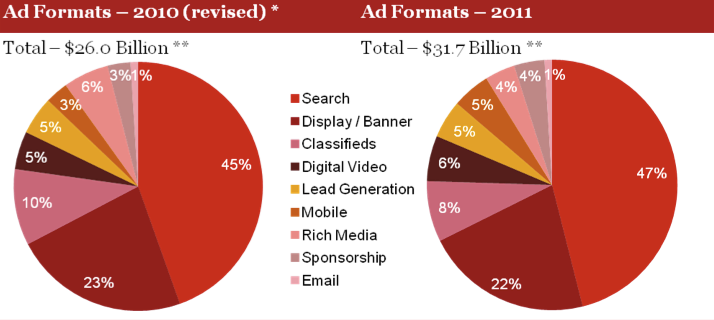
\includegraphics{chapter2.tex/Image0}
  }
\caption{Revenue According to Ad Format \citep[Image credit: ][]{IAB:sv1S8BTo}}
\end{figure}

\begin{sloppier}
Because advertisers are most concerned with efficiently reaching high value consumers (those most likely to buy), targeting is important across all forms of advertising. On the surface, targeting is about breaking the market down into groups, or segments, which share certain characteristics. Typical market segments includes geographic (e.g., region, climate, urban / surburban / rural), demographic (e.g., age, gender, ethnicity, education), contextual (e.g., web page content) and behavioral (e.g., browsing history, content accessed over time). Ideally, advertisers target an advertisement to users most likely to be influenced by it. To accomplish this, advertisers attempt to collect and correlate information about users in order to best segment them. 
\end{sloppier}


Intrinsically, targeting seems linked with profiling and the potential for the accumulation, aggregation, and storage of personal data. Advertising networks claim that such information is anonymous, while consumers and policy makers struggle with the question of whether advertising networks should be entitled to assemble profiles and whether that should entail gaining user permission first. In this balance of this section of Chapter 2, we will put aside privacy concerns and instead focus on:

\begin{enumerate}
\item What it means to track users and why this is important;
\item The nature and use of behavioral data in advertising; and,
\item New market opportunities and potential effects.
\end{enumerate}


\subsection{Tracking Users}
\label{trackingusers}

Defining ``tracking'' is a contentious exercise. The World Wide Web Consortium (W3C) Tracking Protection Working Group has been struggling with a definition for over a year (W3C, 2012). But, in its broadest sense, tracking is the collection, correlation, or transfer of data about Internet activities of a particular users, user agent, or device. Tracking may or may not be consensual and the users may or may not be aware of who is tracking, how tracking occurs, or what data is tracked. Tracking in the browser is most commonly associated by the use of HTTP cookies, but other means include IP address tracking, flash cookies (using the Adobe Flash plug-in), and web bugs or beacons (e.g., images retrieved from a third party website). Of potential future concern may be browser fingerprinting  \citep{Eckersley:2010uj},  though it does not seem that advertisers are using this technique now.

Publishers and advertisers alike track user data. Publishers, or first-party, tracking may include very fine-grained information about a user such email address, name, navigation behavior, etc. Personally identifiable information (PII) may be collected with user consent. And companies with both a brick-and-mortar and significant online presence likely combine information about what they know from shopping habits in the store with other data obtained online. More recently, even purely online businesses are able to tap offline data. For example, FaceBook has recently partnered with Datalogix to link online and offline consumer data  \citep{Reitman:2012wc}. 

First party tracking may also be combined with data collected and aggregated by third party trackers. Third party trackers do not communicate directly with a user but monitor a user's actions in other ways. Generally, third party trackers are explicitly given consent to track by a website publisher. But they may also acquire user data via data exchanges and from Internet Service Providers (ISPs; e.g., via deep packet inspection such as that described in  \citealp{Sesto:2008va})  or other vendor sources. It is also possible for trackers to acquire data by taking advantage of security vulnerabilities and via information leakage (as described in  \citealp{Krishnamurthy:2009vh},  for example).

\subsection{The Nature and Use of Behavioral Data in Advertising}
\label{thenatureanduseofbehavioraldatainadvertising}

In fact, how behavioral tracking is accomplished is anything but transparent. The image below in  \autoref{http}  depicts the many HTTP requests called from the New York Times (NYT) homepage in November of 2012. 


\begin{figure}
\centerline{
  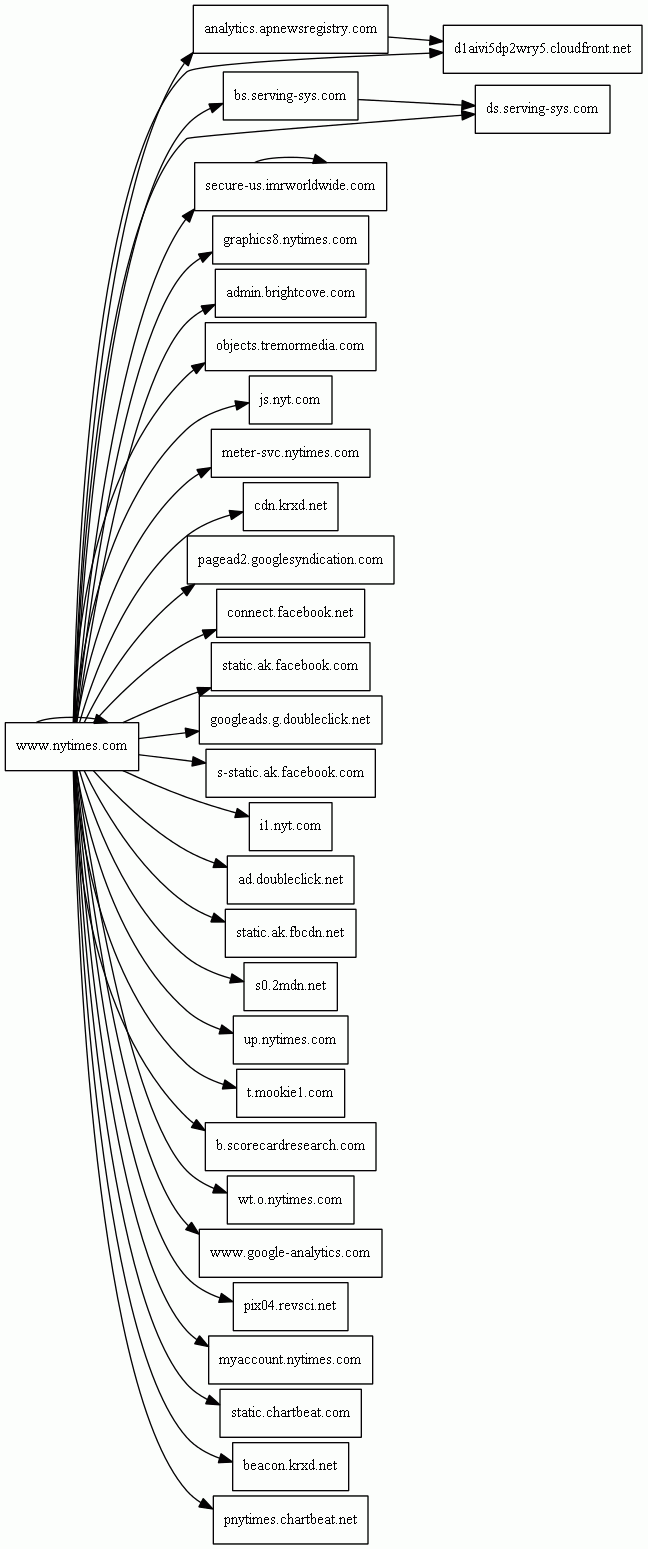
\includegraphics{chapter2.tex/Image1}
  }
\caption{HTTP Requests from the New York Times Homepage}
\label{http}
\end{figure}


A large number of the domains included are third party trackers engaged in analytic or personalization services and advertising. But what makes behavioral tracking feel so insidious is that user activity on one site \emph{can directly influence content displayed in completely un-related sites}. 

For example, on October 5, 2012, after visiting the NYT, Washington Post, and Mozilla home pages, I generated a search query for ``waterproof boots'' on Google search. On October 6, 2012, I refreshed the NYT homepage and was presented an ad for Marc Jacob waterproof boots prominently displayed in the top banner ad space in  \autoref{boots}  below. This may or may not be co-incidence. There is no way to know.


\begin{figure}
\centerline{
  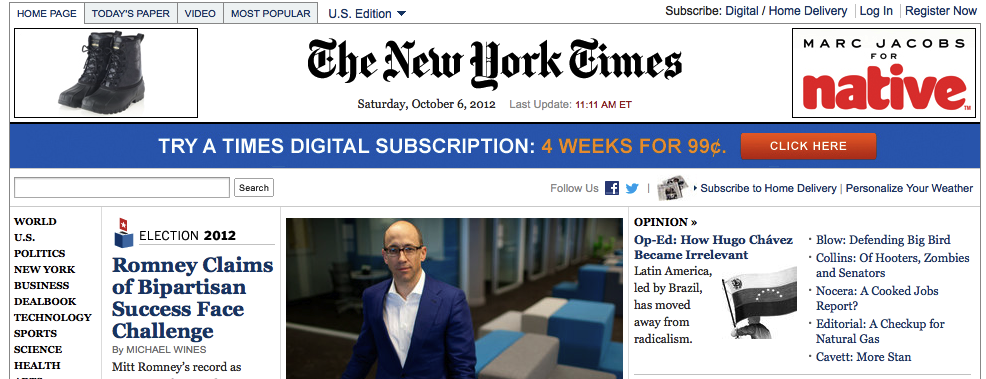
\includegraphics[scale=.75]{chapter2.tex/Image2}
  }
\caption{New York Times Homepage with Advertisement for Marc Jacob Boots}\label{boots}
\end{figure}


A graph diagram generated from the Firefox Collusion extension in  \autoref{collusion}  offers few clues about how my Google query might have caused this ad to be displayed on the NYT homepage. 


\begin{figure}
\centerline{
  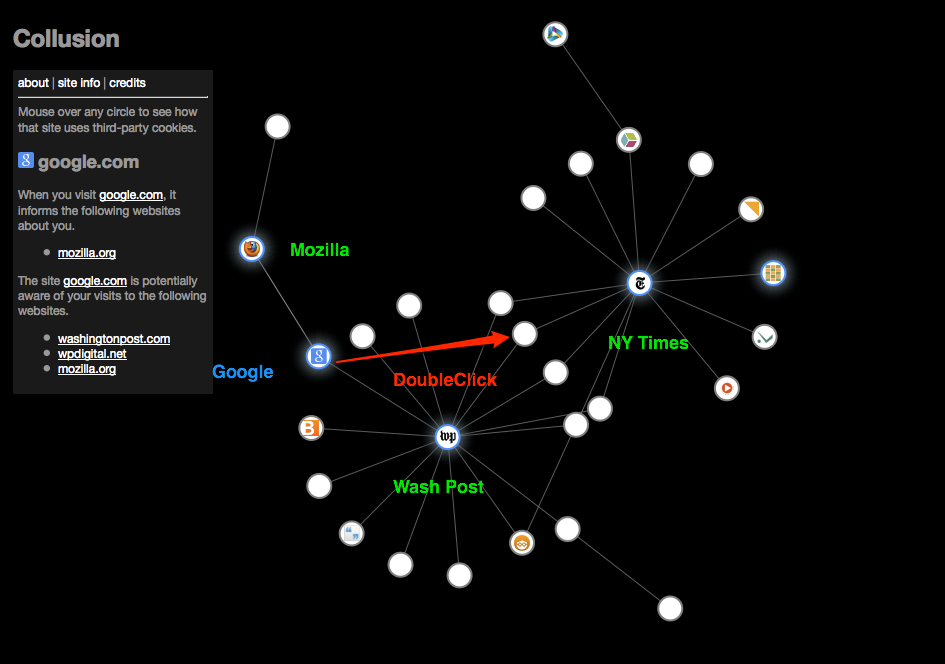
\includegraphics[scale=.75]{chapter2.tex/Image3}
  }
\caption{Firefox Collusion Diagram}
\label{collusion}
\end{figure}


Possibly, Google's advertising subsidiary DoubleClick may have been involved. When seen in the context of this collusion diagram, DoubleClick appears to know of visits to the Washington Post and NYT, but not what search query was made. Yet this is still possible. Business relationships outside of the communicative context also account for data transactions and exchanges.

Behavioral tracking concerns technologies and methods centered on capturing user data when users interact with web content. For example, information captured may include: user visits to a web site, specific page content, visit recency \slash  frequency of visits, links clicked, searches, form data, and other interactive content. This data, plus metadata such as IP address may be combined to create a `profile' linked to that user, browser user agent, or device. The goal of behavioral targeting is to show ads only to users of high value (those who are likely to buy the product) combined with a large number of opportunities to show such ads to that user.

An informal survey of agencies by the IAB suggests that behavioral advertising is widespread: up to 80\% or more of advertising campaigns conducted in 2009 involved some form of tracking  \citep{IAB:2010wz}.  But until recently, we've had little real insight into how businesses, to include advertisers, used behavioral tracking.

In Feb 2012, The New York Times published an article written by  \cite{Duhigg:2012ua}  telling the story of how Andrew Pole, a data scientist in Target's marketing analytics department, developed a model that could successfully predict whether a female customer was in the second trimester of pregnancy.

According to  \cite{Duhigg:2012ua},  there are periods in life when routines and buying patterns change. Advertisers are quick to target customers during major life changes such as the purchase of a house or vehicle, or birth of a child. Retailers are particularly interested in acquiring and retaining new customers during such life changes when habits are more malleable. In the case of a birth event, parents will buy all sorts of items such as maternity clothing and prenatal vitamins --- transitioning to baby care products soon after. Pole began analyzing consumer spending to identify 25 products, in aggregate, predictive of pregnancy and within a narrow window of time. As  \cite{Duhigg:2012ua}  notes, ``it's difficult to attribute how much behavior modeling contributed to Target's revenue, but between 2002 --- when Pole was hired --- and 2010, Target's revenues grew from \$44 billion to \$67 billion''  \citep{Duhigg:2012ua}.  Beyond anecdotal accounts such as pregnancy prediction by Target, there is relatively little information available about how businesses and advertisers profile users through online tracking. 

Not all businesses have such fine-grained information as customer data to enrich predictive models. While Target may have access to name, address, demographics, geography, contact history and many other pieces of information  \citep{HowTargetGetsthe:2010wu},  search engines typically have access to different sorts of data. In  \cite*{Yan:2009dk},  a team from China reportedly published the first academic, and empirical study, to address the question of the whether online behavioral targeting (OBT) can help in online advertising. In this paper, a basic OBT assumption was addressed. The basic assumption is this: ``users who have a similar search or browsing behavior will have similar interests and thus have higher probability to click the same ad than the users who have different online behaviors''  \citep{Yan:2009dk}.  

The team used seven days' ads click-through log data from a commercial search engine recording user search click behavior to include both web page clicks and ad clicks. They represented user behavior by page views and created a behavioral profile by considering all terms appearing in a user's query as previous behaviors. Both users and queries were represented as numerical vectors so that similarity between users could be easily calculated. Using simple clustering techniques, users were segmented according to behavior. Finally, user within-ad similarity was compared with user between-ads similarity. The result was that the within ads similarity, represented by user search behavior, was around ninety times larger than between ads similarity. Thus  \cite*{Yan:2009dk}  concluded that users with similar search behavior would indeed be distinguishable from other users and this could be used to predict the clickability of an ad.

 \cite*{Chen:2009jb}  described ``massive improvements'' in the ability to do offline training of OBT models. They noted, ``behavioral data is intrinsically in large scale (e.g., Yahoo! logged 9 terabytes of display ad data with about 500 billion entries on August, 2008)'' with a sparse click through rate (CTR) of about 0.05\%  \citep{Chen:2009jb}.  To build the entire 450 OBA category models from Yahoo! on fine-grained (ad clicks and search queries) at this scale would take about a week before the innovations they describe were implemented. By using a MapReduce learning algorithm, improved feature vector generation algorithm, better in-memory caching, and more efficient data structures and models they were able to reduce offline model building to about one day.

Scarcely a year later,  \cite*{PandeyΟ:2011ug}  demonstrated the ability to include even more behavioral context to achieve, what they describe, as better results on live data. They created a general purpose model which allowed for optimizing three strategies of behavioral targeting: property (document context), segment (user demographics), and behavior (user past behavior). Each strategy was estimated to successively encode deeper context, thereby potentially improving the richness of the model. User events were modeled as an event stream of three types of events: pages visited, search queries, and graphics ads. By modeling in this manner, the research team examined the relative performance of specific event types (using extracted features), within specific temporal windows with respect to a variety of advertising campaigns of various types and sizes.
In a live experiment spanning three months, they generated user models spanning eight weeks of user history. For each of four ad campaigns, old models (like those described in the previous two paper described above) and new models received at least 1M ad impressions on a monthly basis. The conversion rate for new models was calculated to be considerably higher than for the older models, ranging from 57\% to 264\% higher.

 \cite{PandeyΟ:2011ug}  note, the problem of predicting clicks and predicting conversion have been split along clear lines of information available to publishers and information available to advertisers. There has been growing pressure from within the ad industry to change this. Moving to payment by conversion is an attractive option for advertisers because: 1) it helps to prevent click fraud; 2) can be used to analyze the effectiveness of the advertisement (was there an actual sales conversion and not just a click); 3) can prevent the user from being inundated by too many of the same ad; and, 4) and is compatible with re-targeting across sites  \citep{PandeyΟ:2011ug}.  Accordingly, advertisers have been recently more willing to share individual responses to ads to publishers since it facilitates the use of conversion-optimized models.

\subsection{New Markets}
\label{newmarkets}

The market of online advertising today is, in fact, much more complex than simple supply (publisher) and demand (advertiser) economics. This model, known as direct buy, was dominant in the early days of online advertising  \citep{Mayer:2012wt}.  By the late 1990's advertising networks emerged allowing advertisers to place ads with many publishers --- and publishers to work with many advertisers --- through a common network. In such a model, it is easier for advertisers to target users along multiple dimensions (e.g., page context, demography, geography, behavior) for ad slots.

The advertising community as a whole sees targeting as an opportunity funnel (see  \autoref{facebook}).  Relating this back to psychology, advertisers are aware that to target effectively, then need to consider consumer:

\begin{enumerate}
\item Daily activities;
\item Online activities and habits; and
\item Research time, whether purchase is online or offline \citep{Anonymous:2010uw}.
\label{opportunity}
\end{enumerate}


There is a clear ``in market'' time of opportunity when users are researching purchase decisions. During this period of time, their behavior changes in predictable ways. For example, initially, the user may broadly review a general product space. Then move to a more comparative or winnowing down of choices. And finally, that consumer will look for a store and make a purchase.

Cookie re-targeting takes advantage of this purchase funnel. Recently, Facebook announced a new Facebook Exchange program, a real-time bidding ad system, where visitors with exchange party cookies can then be shown ads related to their web browsing when they return from those sites to Facebook  \citep{Constine:ut}.  The basic idea is to re-target customers that visited a commercial site but did not purchase at that visit. This effectively positions Facebook from working in the broad part of the funnel (demand generation) to the more narrow part of the funnel  \citep[demand fulfillment;][]{Constine:ut}. 


\begin{figure}
\centerline{
  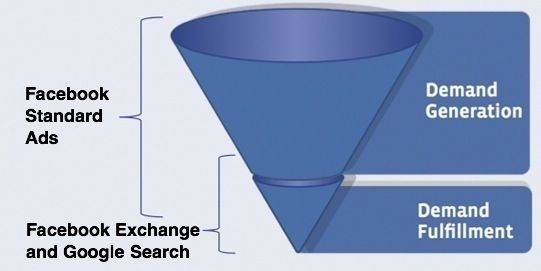
\includegraphics[scale=.75]{chapter2.tex/Image4}
  }
\caption{Facebook Re-targeting \citep[Image credit:][]{Constine:ut}}
\label{facebook}
\end{figure}


To do this, Facebook doesn't share biographical information with advertisers, but takes cookies and combine them with Facebook data  \citep{Constine:ut}. 
The emergence of an \emph{exchange market} --- where buyers and sellers converge --- is attributable to Google's DoubleClick Ad Exchange in 2009  \citep{Duggal:2012tq}.  The perceived value of an exchange over an advertising network is that the exchange operates on the behalf of any number of buyers, sellers, and middlemen alike.  \cite{Anonymous:2012uw}  estimates that real-time bidding exchanges now account for 40\% online data collection. This is up from 0\% three years ago.

Another sort of emergent market is a data market. \emph{Data management platforms} serve as ``a unified technology platform that intakes disparate first-, second-, and third-party data sets, provides normalization and segmentation on that data, and allows a user to push the resulting segmentation into live interactive channel environments''  \citep{OConnell:2011tq}.  Krux  \citeyearpar{Anonymous:2012uw}  found that more than 300 companies collected data on its users, up from 167 companies in 2010. 

Many data collectors also piggyback on each other. By piggy-backing, one tracker invites other trackers to the trough. Because of this, publishers and users may not be aware of how much data is tracked on a given site  \citep{Angwin:2012tg}. 

Not surprisingly, it is difficult to measure the effect of behavioral advertising. Referencing a study from  \cite{Kazienko:2007tb}, \cite{Farahat:2012ex}  observe that click-through-rates (CTR) have declined from 3\% to less than 1\% (since the 1990s). CTR have traditionally been a measure of ad performance, though ultimately, advertisers prefer a more concrete measure such as sales conversions. In the  \cite{Yan:2009dk}  experiment described earlier, ad CTR improvements through behavioral tracking were measured as high as 670\% on the basis of their simple user segmentation strategy from search queries and clicked pages.

However,  \cite{Farahat:2012ex}  question these ad CTR results stating that any study that naively looks at response lifts between targeted and un-targeted groups will greatly overestimate the effects of advertising since there is an inherent selection bias: the targeted users' behavior is likely to be highly correlated with the measured response (``click'').  \cite{Farahat:2012ex}  ask, how do you know that the targeted segment isn't also the most clicky? Since what advertisers care more about are sales conversions than clicks, this is an important question.

In a field experiment on the Yahoo! front page,  \cite{Farahat:2012ex}  try to weed out selection effects in terms of clickiness of the targeted population, brand interest, and category interest. They find strong evidence that user clickiness and brand interest are determinants of variation in CTR. This has bearing on the projected ROI of behavioral advertising for a given campaign. Furthermore, they question the ad CTR improvements of  \cite{Yan:2009dk},  suggesting that the targeted lift of brand-related searches may be over-estimated by almost 1000\%.

 \cite{Farahat:2012ex}  conclude that advertisers would benefit from comparing how targeted and non-targeted populations respond to advertising in any particular campaign in order to gauge the cost effectiveness of their targeting strategy. ``Given an industry average of a three times price premium for targeting, we might conclude targeting is more cost effective, but of course this depends greatly on the targeting product''  \citep{Farahat:2012ex}.  To date, relatively little is published about proprietary behavioral tracking model development nor the effectiveness of such models in actual ad campaigns. Nonetheless, the value of behavioral data is vigorously defended by marketers in public media as ``the fuel the drives the Internet''.\footnote{This is an oft repeated phrase in the media and not attributable to a particular person or source.}

What we really have little understanding is how to deal with the socio-technological effects of the connectedness of many different sorts and bits of data across vast networks of inter-connected participants. Currently, the heavy emphasis is on \emph{who} to target. But there is mounting research to suggest that \emph{when} (in the purchase funnel), \emph{where} (on what site and how the ad should be placed), \emph{what time of day}, \emph{at what geographic location}, \emph{how often}, and \emph{how much} to pay (via auction strategy) are also important to advertisers. Furthermore, with the market moving away from CTR (click through rate) and CTM (cost per mile \slash  ``impression'') towards a sales conversion rate (CVR), there will pressure for even greater information flow between producers and advertisers. Impediments to behavioral tracking become no longer technological, but sociological. And of course, these barriers will fall if both producers and advertisers believe they can profit.

In purely statistically-driven systems, the amount of data, not the algorithm, is king. However, there are many examples of where social network topology provides information that dramatically improves performance over pure volume. When Google created the PageRank algorithm it used page outbound links as implicitly encoded information about what page creators thought important. So what might the effect be when social networks such as Facebook harness vast networks of inter-connected consumers to the problem of behavioral advertising? How likely are we to behave like our friends? Or to what extent can they be used to influence us?\footnote{A NYT article (published Oct. 13, 2012) reports on how the current presidential political campaign is heavily leveraging social and behavioral information to both reach ``in market'' voters as well as pressure them to vote.  \url{http://www.nytimes.com/2012/10/14/us/politics/campaigns-mine-personal-lives-to-get-out-vote.html?pagewanted=1&hp&_r=0} } What if producers and advertisers find secure and effective means of sharing private information about users and their purchasing and other behavior? If the time has not yet come that transactional, behavioral, social, geographic location, and other offline third party data sources are not combined and used by business to more closely target individual consumers --- that time will come shortly.

\section{Privacy and Policy Issues}
\label{privacyandpolicyissues}

Every day, major newspapers across the globe report on some concern over digital data and privacy. Included in this global discussion are talk of law, policy, and technology --- to include threats to privacy as well as proposed solutions. According to  \cite*{Gomez:2009ue},  consumer reports and polls repeatedly show ``overwhelming concern by users about the collection of personal information and behavioral profiling''  \citep[p. 17]{Gomez:2009ue}.  While website publishers typically offer a privacy policy to inform consumers what sorts of data may be collected and how that data may be used or shared, there is nonetheless much confusion and debate regarding what data is considered private and how it is handled. Though how personal data is collected and stored by first-party websites is in question, this section focuses more on the problem of data collected and used by third party trackers as well as public attitude toward this collection. However, in current privacy debates, there has been intrinsically little difference in the stance and attitude between large publishers and advertisers.

\subsection{The Internet is Free}
\label{theinternetisfree}

For some years, the Internet has been a free and open place. Access to services and information has been largely free. While many were initially skeptical about online commerce, convenience and ease won us over. With the advent of mobile technology and GPS, our applications became time and location aware. We can scan barcodes in stores and have applications tell us whether cheaper products are found close by. We embrace the wonder of connecting our virtual lives with our physical lives. But we feel uneasy, as well. The idea of being personally \emph{surveilled} as we move about in the physical world is deeply unsettling --- whether at home or in public. But to be monitored in a web browser leaves open the possibility that strangers will learn, in an intimate sense, \emph{who we are}. They will do this by knowing what we read, what activities we pursue, where we live and travel, where we bank, where we work, what sorts of medical issues we research --- and, naturally, what we buy. This information can be aggregated and stored by strangers --- and then shared with other strangers: without consent, without review.

The delicate balance between public and private life may, in fact, be a relatively recent phenomenon.  \cite{Locke:2010wt}  examines closely the inherent tendencies of biological organisms to eavesdrop on others. Privacy is likened to a ``regulatory process that serves to selectively control access of external stimulation to one's self or the flow of information to others''  \citep[p. 53]{Klopfer:1977ch}.  One of the key functions of privacy is the withholding of information that might provide an opponent with a competitive advantage  \citep{Klopfer:1977ch}.  

In small, egalitarian societies, the ability to constantly monitor and eavesdrop ``rendered trust unnecessary''  \citep[p. 74]{Locke:2010wt}.  Everyone shares access to the same resources. According to Locke, the pervasiveness of eavesdropping serves as a form of social control with an inhibitory effect on behavior. In more complex societies, where walls and buildings function as a sort of social technology, it has become less possible to overhear others and the notion of privacy has became mired with secrecy. At the same time, since one does not know everyone in the community, eavesdropping has become a means for knowing and understanding the private lives of others. Ultimately, ``walls and population increases made it necessary to take in information about others when they were physically absent, relying on the representations --- the gossip --- of intermediaries''  \citep[p. 192]{Locke:2010wt}.  


\subsection{Privacy and Personally Identifiable Information (PII)}
\label{pii}


Dan Solove, a George Washington University Law professor and author of \emph{Understanding Privacy}  \citeyearpar{Solove:2008vz},  frames privacy in terms of legal history and case law. The Fourth Amendment provides for the fundamental right to a ``reasonable expectation of privacy'' to the United States Constitution  \citep[as cited in][p. 2]{Solove:2008vz}.  In Katz v. United States, 1967, the Fourth Amendment protection was extended to include Fourth Amendment protection to public places, such as private conversations in public phone booths  \citep[as cited in][p. 22]{Solove:2008vz}.  However, the Supreme Court observed, ``What a person knowingly exposes to the public, even in his own home or office, is not a subject of Fourth Amendment protection''  \citep[as cited in][p. 22]{Solove:2008vz}. 

In fact, it is the inherent difficulty in resolving what ``privacy'' is, that drove Solove to write his book. He notes ``there is no overarching conception of privacy --- it must be mapped like terrain, by painstakingly studying the landscape''  \citep[p. ix]{Solove:2008vz}.  This is particularly relevant when considering user browser-based interaction with websites over the Internet.

As  \cite{Solove:2008vz}  notes, there are literally hundreds of laws at state and federal levels to protect privacy:

\begin{quote}
Congress has passed several dozen statutes to protect the privacy of government records, student records, financial information, electronic communications, video rental data, and drivers' records, among other things. Furthermore, privacy is recognized as a fundamental human right. According to the United Nations Declaration of Human Rights of 1948, "No one shall be subjected to arbitrary interference with his privacy, family, home or correspondence, nor to attacks upon his honor and reputation." \citep[p. 3]{Solove:2008vz}.
\end{quote}

At particular risk or bits of information known as ``personally identifiable information'' (PIIs) typically associated with harms such as identify theft and mis-use. In May 2007, the Deputy Directory of the Office of Management and Budget (OMB) sent a memorandum on the subject of ``safeguarding against and responding to the breach of personally identifiable information'' noting,

\begin{quote}
The term "personally identifiable information" refers to information which can be used to distinguish or trace an individual's identity, such as their name, social security number, biometric records, etc. alone, or when combined with other personal or identifying information. \citep{OMB:2007vu}
\end{quote}

The purpose of this memorandum was to reinforce requirements of the Privacy Act of 1974 to both safeguard and establish rules of conduct for the handling of personally identifiable information. The particular challenge was in response to the ease to which technology has made it possible to personally identify particular individuals by combining small pieces of information. It is not that this is a new challenge: for example, brick-and-mortar businesses have long asked customers for a zip code when a customer pays with a credit card. These two pieces of information can be easily combined to find a home address. What's changed is that technology and the Internet has made it far easier to identify and, potentially harm, users at vast scale. And the idea of PII now seems to extend to seemingly innocuous bits information such as Internet browsing behavior. What was once viewed as categorically deterministic is now probabilistic in terms of re-identifiability and risk.

\subsection{Growing Public Awareness}
\label{growingpublicawareness}


\begin{quote}
\textbf{Steward Cheifert} (Interviewer): How concerned should I be as a user about what I put up on the Net?

\textbf{John Markoff} (West coast correspondent, New York Times): I think it depends on what you do. There's better security coming for economic business transactions, but I'd be careful about putting my password on the net, I'd pick a password that's a safe password, and I wouldn't put my credit card up until there is security software up that will protect my credit card. \citep{TheInternet:uu}
\end{quote}


In the early 1990's, the Internet exploded into public awareness. 1993 signaled the first graphical web browser and the world was mesmerized. There was a growing excitement for interaction on the World Wide Web, and public talk was dominated by the promise of possibility. The large concern was whether it was safe to shop online --- though the focus was on the encryption of credit card transactions, rather than the seemingly benign micro-exchanges of a user clicking through web pages. 

In November of 1999, DoubleClick, an advertising network of over 11,000 publishers, purchased Abacus Direct a company maintaining a database of detailed consumer profiles on approximately 90\% of American households  \citep{Anonymous:Hkl3lUXG}.  DoubleClick announced that it planned to merge ``anonymous'' online data (100 million user profiles) with Abacus profiles (including names, addresses, phone numbers, etc.). The media roiled and public sentiment was overwhelmingly negative. Ultimately, DoubleClick put these plans on hold: it's stock dropped dramatically after the merger was announced since neither the public nor Wall Street had reacted favorably to this plan  \citep{Anonymous:1999wh}.  It was about this time that the public became aware of how their behavior on the Internet might be used by commercial entities. A Federal Trade Commission (FTC) investigation in 2001 ended its investigation with no finding that DoubleClick had engaged in unfair or deceptive trade practices. It concluded:

\begin{quote}
Based on this investigation, it appears to staff that DoubleClick never used or disclosed consumers' PII (personal identifiable information) for purposes other than those disclosed in its privacy policy. Specifically, it appears that DoubleClick did not combine PII from Abacus Direct with clickstream collected on client Web sites. In addition, it appears that DoubleClick has not used sensitive data for any online preference marketing product, in contravention of its stated online policy \citep{Anonymous:Hkl3lUXG}.
\end{quote}

This case, and others like it, now had the public's eye. By the year 2000, 54\% of Americans used the Internet at home  \citep{Simms:2000vo}.  In a March 2000 poll, 82\% of web users polled indicated that they were uncomfortable if their browsing habits and shopping patterns were linked to their identities  \citep{Anonymous:te}.  74\% indicated that they were very uncomfortable if their information were sold to other organizations. Though only 40\% of users had heard of browser ``cookies'', many were aware that data was being collected silently and that data could be both sold and merged with identifiable information. Public negative sentiment toward tracking has changed little over the years. Over 70\% in 2012 say they find little value in online ads  \citep{Hoofnagle:2012uc}.  And Microsoft reports that 75\% of its US and European users would like to opt-out of online advertising  \citep{Hill:2012uh}. 

\subsection{Third-Party Data Collection}
\label{third-partydatacollection}

Browser tracking is not the only means by which websites identify and collection user information. But it's, perhaps, the sort of data collection people are intuitively least comfortable with. Third-party trackers are trackers on websites that collect information about users for a third party. They are not officially part of the website visited, but are generally associated with advertisers or web analytics. Typically, they take the form of cookies. Cookies can be set by embedded JavaScript and allow a site to essentially ``remember'' arbitrary bits of information from a previous session. Advertisers can utilize cookies in a cross-domain manner by creating a unique ID that is set by one website and then picked up by that same advertiser on another website. In this way, the advertiser knows that you've visited both sites. 

The problem with cookies is that it is a browser-mediated information exchange \emph{hidden from view}. Some cookies serve useful functions for sites with which we have trusted relations. But many are set and tracked by organizations that we may not recognize and for purposes that are unclear. Of great concern is that these entities may be buying, selling, and trading browser profiles which can be linked to personally identifiable information (PII).
 \cite{Narayanan:2011tv}  proposed a five-fold taxonomy in which browsing history might become pseudoanonymously\footnote{``Psuedoanonymous'' unique IDs may be used to identify a particular device or user agent. These may potentially be linked to other, personally identifying information later.} identifiable to a particular device or user.

\begin{enumerate}
\item \textbf{The third party is sometimes a first-party.} A third party tracker such as Facebook may be a first-party in other contexts. If you visit Facebook and login, it sets a cookie that can be used to track you as you browse the web. \cite*{Roesner:2012uj} describe the particular situation where sites have buttons such as Facebook, Twitter, or Google embedded on their web pages. These buttons are trackers and used to track you even if you never click on them. If you visit a website, and are also logged into Facebook in the same browser, Facebook will know that you've visited that site.
\item \textbf{A first party leaks data to third-parties.} \cite*{Krishnamurthy:2011uv} found that 56\% of 100 popular, non-social network sites leaked private information. This number grows to 75\% if a site userid is included as a PII.
\item \textbf{A first party sells the user's identity.} The previously mentioned case of Abacus and DoubleClick serves as a good example. Also, \cite{Narayanan:2011tv} notes that survey sites (e.g., "win a free iPod!") can also act as an identity provider to sites on which they have a third-party presence.
\item \textbf{Hacks and exploits.} A third-party might exploit a cross-site vulnerability on a first-party website to learn the user's identity \citep{Narayanan:2011tv}.
\item \textbf{Deanonymization (re-identification).} A third party could match browsing histories against datasets to re-identify particular persons, as \cite{Narayanan:2010kb} did with the Netflix Prize dataset. In this experiment, they demonstrated that it's possible to identify a particular subscriber with only a little bit of information.\footnote{In fact, this is only one example of many. Re-identification is another huge challenge for privacy law. For discussion in greater depth, see \citet{Ohm:2010vj}.}
\end{enumerate}

Though Netscape never intended cookies to be privacy-invasive, enterprise-minded businesses quickly realized that cookies could be used for identifying browsers. In fact, the ecology of tracker technology in the wild is surprising complex and, potentially, adaptable.

 \cite{Roesner:2012uj}  performed a study in which they observed tracker behavior from the point-of-view of the client browser. They classified this behavior into five behavioral patterns in which a given tracker site might exhibit variable behavior depending on contexts. They note complex behaviors such as that of an aggregate tracker referring data to other trackers. A few trackers stored data in multiple locations simultaneously (e.g., cookies, flash storage, HTML5 local storage) or exhibited spawning behavior when cookies were cleared. When they asked the question of how much data can any one tracker could collect, using 2006 AOL search query data, they found that, on average, DoubleClick could track a user across 39\% of pages visited, and a maximum of 66\% of pages visited.

Though cookies are the most prevalent trackers, ``web bugs'' serve a similar function. They are traditionally embedded as small (often 1 pixel) GIF or PNG images and can also be used in HTML mail, informing advertisers whether an email has been opened and when. In March 2010, Ghostery identified 117 unique web bugs on nearly 400,000 unique domains  \citep*{Gomez:2009ue}.  Though privacy policies may state that information will not be shared with third parties, many of these sites nonetheless allow third-party tracking through web bugs  \citep{Gomez:2009ue}. 

Given the complex behavior of trackers, coupled with complex business practices in which first-parties and third-parties may mingle or exchange data, it is not surprising that users may be confused about who has collected, stored, traded, or used their browsing profile.

\subsection{Cookies and Privacy Law}
\label{cookiesandprivacylaw}

Recent litigation over OBT invokes Wiretapping acts both federal and state. At the federal level, the Electronic Communications Privacy Act (``ECPA'') Wiretap Act, Stored Communications Act (``SCA''), and the Computer Fraud and Abuse Act (``CFAA'') are frequently invoked. 

The federal Wiretap Act (as amended by the ECPA) protects the privacy of wire, oral, and electronic communication. The latter is defined as ``any transfer of signs, signals, writing, images, sounds, data, or intelligence of any nature transmitted in whole or in part by a wire, radio, electromagnetic, photoelectronic or photooptical system''  (\citeauthor{Anonymous:ux}).  Under  \S  2511(3), ``a person or entity providing an electronic communication service to the public shall not intentionally divulge the contents of any communications{\ldots} while in transmission on that service to any person or entity other than an addressee or intended recipient{\ldots}'' 

The ECPA has been criticized lately by the media:

\begin{quote}
Many Internet companies and consumer advocates say the main law governing communication privacy --- enacted in 1986, before cellphone and e-mail use was widespread, and before social networking was even conceived --- is outdated, affording more protection to letters in a file cabinet than e-mail on a server." \citep{Helft:2011wx}
\end{quote}

Such criticism had been directed at Government data requests, yet numerous cases solely involving commercial entities  abound.\footnote{For example, "In re Doubleclick, Inc." and others referenced at \url{http://www.internetlibrary.com/topics/electronic_cpa.cfm}.}  Of issue for OBT is an exception known as the \emph{consent exception}: so long as one of the parties of electronic communication has given prior consent to the interception, and the interception was not intended for criminal or ``tortuous act'', then it is exempt from the Wiretap Act  \citep{Anonymous:2008vj}.  

One notable case which invoked ECPA, SCA, and CFAA was the case of ``In re Doubleclick, Inc.''. In 2000, a class action suit was brought against Doubleclick Inc., which used cookies for behavioral advertising. With respect to ECPA Wiretap law, Doubleclick successfully argued that its affiliated websites were ``users'' of the Internet and that communications accessed by Doubleclick's cookies were ``of or intended for'' these websites  \citep{Anonymous:Hkl3lUXG}.  The Stored Communications Act was found not to apply to Doubleclick, as well. The SCA was intended to address temporary and transactional records of internet service providers. Cookies stored on personal hard drives and were out of scope for the intent of SCA  \citep{Anonymous:Hkl3lUXG}.  Finally, with respect to the Computer Fraud and Abuse Act, the plaintiff failed to provide evidence that they had incurred harm.

As it stands today, federal laws do not address concerns raised by online behavioral tracking on the Internet. Furthermore, given the single-party consent exemption of Federal Wiretap law, communications between Internet users and websites is not private if the website owner has given its consent for monitoring.

\subsection{Policy Legislation - Do Not Track}
\label{policylegislation-donottrack}

Though the United States does not have specific federal law that applies to behavioral tracking, the Federal Trade Commission (FTC) can enforce the terms of privacy policies under Section 5 of the FTC Act prohibiting ``unfair or deceptive'' marketing practices  (\citeauthor{Anonymous:vq}).  This applies to FTC handling of behavioral tracking. In 2011, the FTC found three parties in violation for the FTC act relating to third-party tracking  \citep{Mayer:2012wt}.\footnote{A violation is determined if a company states in a website notice or privacy policy that it does not engage in a particular practice, when in fact it does.} 

In 2010, the Federal Trade Commission proposed ``do not track'' technology as ``likely a persistent setting on consumers' browsers --- so consumers can choose whether to allow the collection of data regarding their online searching and browsing activities''  \citep{Anonymous:2010ti}.  This represents a form of self-regulation insofar that trackers are expected to respond appropriately to browser requests not to track. In its March 2012 report  \cite{Staff:2012th},  the FTC outlined a broader privacy framework to address a myriad of concerns surrounding data brokering, mobile, internet service providers, and enforceable self-regulatory codes. The scope of this framework applies to:

\begin{quote}
[...] all commercial entities that collect or use consumer data that can be reasonably linked to a specific consumer, computer, or other device, unless the entity collects only non-sensitive data from fewer than 5,000 consumers per year and does not share the data with third parties. \citep{Staff:2012th}
\end{quote}

The FTC notes that this framework applies to offline as well as online data and applies to data that is reasonably linkable to a specific consumer, computer, or device.

As proposed by FTC  \citep{Staff:2012th},  Do Not Track should include five key principles:

\begin{enumerate}
\item It should be implemented universally to cover all parties that would track consumers. 
\item The choice mechanism should be easy to find, easy to understand, and easy to use. 
\item Any choices offered should be persistent and should not be overridden if, for example, consumers clear their cookies or update their browsers.
\item It should be comprehensive, effective, and enforceable: it should opt consumers out of behavioral tracking through any means and not permit technical loopholes.
\item It should go beyond simply opting consumers out of receiving targeted advertisements; it should opt them out of collection of behavioral data for all purposes other than those that would be consistent with the context of the interaction (e.g., preventing click-fraud or collecting de-identified data for analytics purposes; \citealp{Staff:2012th}).
\end{enumerate}

Since the FTC released its preliminary findings, the W3C Internet standards body convened a working group toward the adoption of an industry-wide Do Not Track standard. This group includes representatives from the advertising industry, online businesses, academia, privacy advocates --- both nationally and internationally. The challenge for this group is to devise a standard that meets FTC guidelines, while satisfying a diverse array of agendas.

\subsection{Building Privacy Policies into Browser Protocols}
\label{buildingprivacypoliciesintobrowserprotocols}

In the late 1990s, there were a couple of attempts to address the problem of privacy invasion introduced by third-party cookies via technical means. Introduced in 1997, RFC 2109 was a proposal aimed at putting strict controls on cookie usage. Commercial entities participating in standards discussion objected to portions of this proposal and it was, ultimately, not supported by browser developers. ``Where the browser manufacturers had been asked to redesign their software to reject cookies automatically, Netscape and Microsoft Internet Explorer instead included options for users to reject cookies if they so chose''  \citep{Eichelberger:um}.  As cookie inventor Lou Montulli stated, ``browser default would still be set to accept cookies, since it was felt by the designers that if we were to unilaterally disable this feature, existing content on the Web would no longer work''  \citep{Bruner:1997ti}. 

From 1998 - 2003, the W3C organized a standards committee to propose a Platform for Privacy Preferences (P3P) standard  \citep{Schwartz:2009tc}.  The standard aimed to create a machine-readable policy that captured the complexity of human-readable privacy policies and boiled them down to a multiple-choice set of options. What resulted from long and heated discussion was highly controversial and touted as overly complex --- and unlikely to be adopted as a self-regulatory option with no degree of enforcement.

About the same time, advertisers began to take a more active role in self-regulation. The National Advertising Initiative (NAI) set up a website to allow users to download opt-out cookies for participating networks. Their principles have been to notify users and allow them a choice. Opt-out does not mean that you will not be tracked or that ads will not be served. It means that ads will not be tailored to your browsing behavior. Opt-out choices are stored in browser cookies, so they recommend to visit their opt-out page periodically for updates. 

Other advertising networks and companies have since also offered similar opt-out cookie  services.\footnote{For example, see \url{http://www.worldprivacyforum.org/cookieoptout.html}.}  Large advertising industry groups formed a new parallel self-regulatory program for behavioral advertising, the Digital Advertising Alliance (DAA). The DAA and the Interactive Advertising Bureau (IAB), a self-regulatory for advertising networks, advocate the use of an advertising option icon to be displayed on web pages with tracking scripts. A user who clicks on the icon sees a disclosure statement and can click through to an opt-out page. However, according to a 2011 study at the Center for Internet and Society at Stanford University, only 11.3\% of members to date offer cookie-based opt-out.  \citep{J:2011wm}. 

In 2007, the Center for Democracy and Technology (CDT) sent a note to the Federal Trade Commission (FTC) requesting that ``the online tracking and targeting of consumers --- both in its current form and as it may develop in the future --- needs to be limited so that consumers can exercise meaningful, granular preferences based on timely and contextual disclosures that are understandable on whichever devices consumers choose to use''  \citep{CenterforDemocracy:uc}.  They called for a national Do Not Track list similar to the national Do Not Call list. Their proposal called for a machine readable list of the domain names which used cookies and other means to track users. Browsers and third party software could then use this list in order to limit tracking  \citep{CenterforDemocracy:uc}. 

Thus, the W3C chartered the Tracking Protection Working Group (TPWG) ``to improve user privacy and user control by defining mechanisms for expressing user preferences around Web tracking and for blocking or allowing Web tracking elements''  \citep{Anonymous:vz}. 

In effect, discussion in this group mirrors, and perhaps fuels, public debate in media and society.\footnote{The public-tracking list is archived at:  \url{http://lists.w3.org/Archives/Public/public-tracking/}. } Chairs for the group serve to organize and moderate debate. As questions become more defined, formal ``issues'' are raised and ``actions'' assigned to particular members. For example, ISSUE--5, ``What is the definition of tracking?'' was opened on September 21, 2011. As of October 2013, there are 446 emails pertaining to this issue alone, and it is still open more than two years later. 

Because each member has his or her own platform or stance on any particular matter, debate sometimes bleeds into other venues. For example, as of this writing, the current DNT draft standard says the following (regarding determining a person's DNT preference): ``A user agent must have a default tracking preference of `unset' (not enabled) unless specific tracking preference is implied by the decision to use that agent''  \citep{Anonymous:uk}.  When TPWG member Roy T. Fielding, who works for Adobe but who also contributes to the open source Apache webserver codebase, committed a patch to this codebase which disabled DNT if the browser requesting data was Internet Explorer 10 (which at the time set DNT to 1 by default), he caused a ripple tide of effects. His patch, labeled ``Apache does not tolerate deliberate abuse of open standards''  \citep{Fielding:2012wh},  clearly reflects his own position on the implementation of DNT. This hit C\slash NET news and Twitter almost simultaneously. On Twitter, Jonathan Mayer  \citep{J:2012uz},  fellow TPWG member responded with  \autoref{tweet1}. 

\begin{figure}
\centerline{
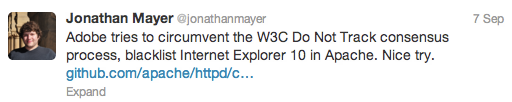
\includegraphics{chapter2.tex/Image5}
}
\caption{{Tweet, 7 September 2012}}
\label{tweet1}
\end{figure}


About the same time, C\slash NET reported the event, noting Roy T. Fielding's position as an author of the DNT standard and principal scientist at Adobe Systems  \citep{Shankland:tz}.  Of course, there was an immediate back-lash on the public-tracking list between Mayer and Fielding, in which Mayer  \citep{J:2012vq}  partially retracted his comment on Twitter  \autoref{tweet2}. 


\begin{figure}
\centerline{
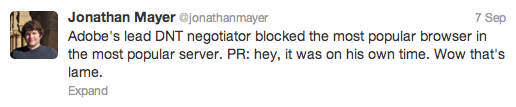
\includegraphics{chapter2.tex/Image6}
}
\caption{{Tweet, 7 September 2012}}
\label{tweet2}
\end{figure}


From Fielding on the public-tracking list:

\begin{quotation}
Our charter forbids us from specifying UI requirements. That does not mean any of the following excerpts are ambiguous:     

A user is an individual human. When user-agent software accesses online resources, whether or not the user understands or has specific knowledge of a particular request, that request is made "by" the user.

The goal of this protocol is to allow a user to express their personal preference regarding tracking to each server and web application that they communicate with via HTTP ...    

Key to that notion of expression is that it MUST reflect the user's preference, not the choice of some vendor, institution, or network-imposed mechanism outside the user's control. The basic principle is that a tracking preference expression is only transmitted when it reflects a deliberate choice by the user. In the absence of user choice, there is no tracking preference expressed. \citep{Fielding:2012vf}
\end{quotation}

On the basis of this personal conviction, Fielding argued that if DNT was switched on by default, it should be ignored, regardless of other considerations. Since Microsoft had announced that it would turn on DNT by default, Fielding retaliated using the technological means at hand --- direct modification of code. Naturally, this led to heated debate within the Apache http server developer community. As of this writing, there were 364 comments on this commit. Fielding's changes are reflected in the current configuration of the main branch of code, but are commented out.

Lorrie Craner, one of the original developers of P3P is skeptical that DNT will succeed. To her it seems a simpler, but not better, replay of the P3P proposal  \citep{Staff:2012th, Fulton:2012ti}. 

\begin{quote}
As we walk about in the physical world, we raise and lower our voice and we raise and lower our window shades and we turn our faces, and we are all constantly adjusting to regulate our exposure and our privacy, Dr. Cranor tells RWW. "And it comes naturally; we don't spend a lot of time thinking about it. We just sort of naturally do it. But when we go online, it's no longer natural, because we don't have these readily apparent, physical things where you can just easily close that shade, and it's obvious what you're doing. So we have to rely on software tools to help us with this privacy regulation process. \citep{Fulton:2012ti}
\end{quote}


\subsection{Choice and Self-Regulation}
\label{choiceandself-regulation}

While policy debate rages, the advertising industry continues to advocate self-regulation. Central to self-regulation is the notion of choice. The DAA and NAI naturally view behavioral advertising in a very positive sense such that better targeted ads are preferable to ads that do not match a consumer's interests. But if a user does not wish to participate, then they should have the choice to opt-out. However, privacy advocates cite two large concerns with respect to industry self-regulation.

The first argument against the effectiveness of self-regulation is non-compliance. A Carnegie Mellon University (CMU) report by  \cite*{Komanduri:2012wo}  finds that, despite attempts at self-regulation by bodies such as the DAA and NAI, there are still many examples of non-compliance. Stanford University website  \url{http://donottrack.us}  believes that further steps are required: namely, regulation enforcing compliance with user choice. 

A second, perhaps more compelling argument is that the advertising industry relies on technologies that seem to ensure that users remain unaware of them. When consumers attempt to block tracking, other more resistant methods are developed which circumvent these defenses. While DNT would make it very easy for users to decide not to be tracked, market choice seems to make it easier for them to be tracked. As  \cite*{Hoofnagle:2012ve}  note, ``those who argue that consumers can negotiate the nuances of privacy and tracking online assume that the online world is similar to the offline world.'' In the offline world the consumer can leave without leaving behind a data trail. But in the online world, invisible attributes leave marks that are easy to follow. They further note that surveys of top websites in 2009 and 2011, revealed new tracking mechanisms resistant to the strongest of privacy settings. Or, perhaps, advertisers simply know that once online shopping is habit, consumers will adapt.

\subsection{Opt-In Versus Opt-Out}
\label{opt-inversusopt-out}

On the 26th of May 2012 in the U.K., a new European Cookie Law, E-Privacy Directive 2009\slash 136\slash EC, came into effect.\footnote{There is a high-level summation here:  \url{http://gigaom.com/europe/cookie-law-explainer/}. } This law requires the consent of users before cookies are set (see  \autoref{cookie-notification}).  In effect, this is an unequivocal ``opt-in'' system of notification and consent (with the exception of cookies ``strictly necessary'' for the operation of a website  \citep{Anonymous:2009uu}.  


\begin{figure}
\centerline{
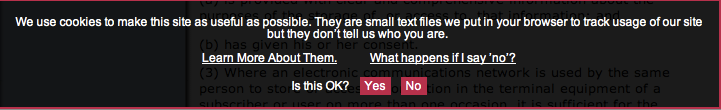
\includegraphics[scale=0.70]{chapter2.tex/Image7}
}
\caption{Example cookie opt-in notification from: \url{http://www.jonwallacedesign.com/privacypolicy.html}}
\label{cookie-notification}
\end{figure}


Unlike current trends in US policy and law, this puts the burden of consent on the website publisher --- not the user. Though this issue permeates the entire European Union (EU), discussion of the UK ``Cookie Law'' requirement for consent has finally reached US audiences on the Internet. 

Perhaps, this EU Directive gives a sense of what may be required if US lawmakers decide to place the burden of consent on website publishers and not users. Such a shift would also acknowledge that Internet transactions between users and websites are currently not ``private'' as Federal Wiretap law has held. The EU Directive seems more in line with user expectations, but given current criticism on the difficulty with compliance, falls short with respect to implementation. The hope is that the W3C Tracking Protection Working Group (TPWG) will provide strong enough guidance to satisfy this Directive. However, US members (and especially those representing business interests) may decide to act in an insular fashion and have, thus far, shown little motivation to join a more global debate  \citep{WCpublictracking:mGxHNO_D}.  

\section{User Confusion}
\label{userconfusion}

There has long been an asymmetry in communication between web publishers and users. Interactive page elements such as ``contact us'' via web forms, instant chat, web forums, and email have enabled users to connect directly to persons behind the scenes. More recently, publishers utilize personal messaging through other channels such as Twitter, Facebook, or SMS for allowing users to offer direct and personal feedback. These are direct and intentional communications between parties. But the act of visiting a webpage in itself also has communicative value. 

In this section, I highlight user confusion regarding indirect communications where advertisers and other commercial actors silently monitor web interaction via the use of cookies. Not only is the phenomenon of behavioral tracking difficult to understand and see, but user defenses against ubiquitous monitoring are confusing, as well. Of particular interest are user opt-out mechanisms provided for by emerging DNT standards and also the advertising industry efforts toward self-regulation of online behavioral advertising. The vehicle for this is ``consumer choice'' and the Advertising Option Icon (viz. AdChoices icon; see  \url{http://www.aboutads.info} for general information).  

\subsection{Confusion About Third Party Tracking}
\label{confusionaboutthirdpartytracking}

In a 2009 study of Internet user understanding of behavioral advertising,  \cite{McDonald:2009vz}  found that only 51\% believed that the ability of an ad company to determine which ads to show them based on the history of prior websites they visited was something that ``happens a lot right now'' \citep{McDonald:2009vz}.  46\% of the same study participants found the idea of behavioral advertising ``creepy'', and another 40\% agreed or strongly agreed they would be more careful online if they knew advertisers were collecting data.

In the virtual online world where billions of people have access to the web through the view of what may often be a personal device, it's not surprising that the experience feels, to some degree, private. As privacy advocate Christopher Soghoian remarks,

\begin{quote}
Consumers treat the search engine box like their psychiatrist, their rabbi, their priest, their doctor. People type the most intimate things into search engines and other websites primarily because they think they're anonymous. They type in things on WebMD that sometimes they wouldn't even ask their own doctors... And in fact, we are not anonymous, these sites are tracking us." \citep[as cited in][]{Kessler:2010vq}
\end{quote}


The UC Berkeley School of Information KnowPrivacy Project  \citep{Gomez:2009ue}  looked specifically at user concerns and knowledge. They examined 50 of the most visited websites and their privacy policies. They also considered specific practices such as third-party tracking and sharing with affiliates. Not surprisingly, they found that most users are concerned about data collection on themselves and their control over that collection and use of information. Furthermore, they found overwhelming evidence (from prior surveys) that users lack knowledge and understanding about data collection practices and policies.

Once source of obvious confusion has to do with terminology. What is tracking? Does that include collection? Most users think not  \citep{McDonald:2011vx, McDonald:2011uv}.  What is the difference between ``third party'' and ``affiliate''? Privacy law treats these categories differently: third-party information sharing is subject to more restriction. According to  \cite{Gomez:2009ue},  websites make distinctions between sharing with affiliates and third parties. 29 of 50 companies examined state that they do not share data with unrelated third parties, 45 state that they share data with affiliates, and 36 state that they allow third-party tracking. This last category falls outside of privacy policy coverage. As  \cite{Gomez:2009ue}  note, it's very unclear what it means to not share data with unrelated third parties yet permit third party tracking.

Despite assurances that affiliates and third parties are treated differently, website providers often leak personal information to the less trusted, embedded third party trackers such as username, login time, and other information. Just as troubling is that users have no practical way of knowing who affiliates are and what sorts of information are passed to them. In the Know Privacy Report  \citeyearpar{Gomez:2009ue},  many of the websites examined are owned by companies with hundreds of subsidiaries: NewsCorp has over 1500 subsidiaries while Bank of America has over  2300.\footnote{These numbers reportedly do not include subsidiaries of subsidiaries.}  The pervasive presence of third party trackers on the Internet means companies have ample opportunity to construct long term profiles of things we do online.

Privacy policies often go unread, or may be difficult to understand  \citep{Milne:2004dy, Sherman:2008uz}.   \cite{Fernback:2007bq}  conducted an in-depth discourse analysis of privacy statements of three large companies. They also noted discrepancies regarding the use of the term ``third-party''. From their study of the Real Network privacy policy: ``We will never sell, rent or disclose to third parties our customers' personally identifiable information {\ldots} gathered on a RealNetworks Website unless we are required to do so by law or receive your advance informed consent''  \citep{Fernback:2007bq}.  Yet, in what appears a blatant contradiction, later in the same privacy policy:

\begin{quote}
Your personally identifiable information may be transferred in connection with a sale, merger, transfer, exchange or other disposition (whether of assets, stock or otherwise) of all or a portion of a business of RealNetworks, Inc. and/or its subsidiaries. \citep{Fernback:2007bq}
\end{quote}

In general,  \cite{Fernback:2007bq}  note that privacy policies are seen to protect the company and typically avoid mention of specifics such as precisely what information might be collected and for what purpose. Given that the FTC has a history of prosecuting companies that violate their terms of  agreement,\footnote{See \url{http://www.ftc.gov/os/caselist/index.shtm} for example. Google and Facebook have both earned penalties.}  this is not terribly surprising. 

 \cite*{McDonald:2009vz},  examined the readability of online privacy statements. They examined standardized text formats and compared these to free text policies. They found that experiment participants could more readily read and comprehend standardized formats, but at the expense of accuracy. And users, in general, did not like either standardized or free text formats. But when it comes to purchasing privacy-sensitive items,  \cite*{Egelman:2009ut}  found that users actually paid attention to graphical privacy indicators.

\subsection{Confusion about Defenses}
\label{confusionaboutdefenses}

When it comes to defending against third party tracking and privacy, users have a number of choices.  \cite{Roesner:2012uj}  identified the following options:

\begin{itemize}
\item \textbf{Pop-up blockers:} Pop-up blockers can stop trackers from forced pop-ups, but there are similar methods such as site re-directs that may not be stopped;
\item \textbf{Browser third-party cookie blocking:} Many third party cookies can be blocked if users select third-party cookie blocking in their browers. However, this will not stop the sort of tracking when a Facebook tracker is accepted as a first-party tracker and its role changes later to a third-party tracker; 
\item \textbf{Private browsing:} Private browsing mode was designed to protect users from having their browse state examined by physical access. But it does not keep browsing state from being examined online;
\item \textbf{Opt-out cookies (and AdChoice icon):} The Digital Advertising Alliance (DAA) is an industry funded policy group that hosts an opt-out web page. From this page, users can click a button to set opt-out cookies;\footnote{There are other similar sites that offer opt-out cookies. For example, Evidon Global, and others have web pages with such links.}
\item \textbf{Clearing browser state:} Clearing cookies when closing the browser is a simple means to reduce the effects of tracking. However, this may also remove opt-out cookies and is also not effective against re-identification by trackers such as the Facebook like icon when logged in;
\item \textbf{Do not track (DNT):} The proposed FTC "Do Not Track" DNT policy is designed to give users a way to opt out of web tracking. This is accomplished via an http request header with a DNT=1 header to inform the remote server that the client wishes to opt out. DNT is not mandatory and requires no compliance. The DAA has committed only to stop content personalization, if it receives a DNT signal. (\url{http://www.aboutads.info/choices/}); and,
\item \textbf{Blocking plug-ins:}  There are a number of browser plug-in which are designed to block trackers.
\end{itemize}

Lorri Craner directs the CyLab Usability Privacy and Security (CUPS) Laboratory at Carnegie Mellon University. She and her students have conducted a series of studies centered on user understanding of online behavioral advertising and usability of blocking tools  \citep{McDonald:2010vv,Ur:2012ws,Leon:2012vu,Cranor:2012ui}. \cite{Leon:2012vu}  studied the usability of Ghostery, Adblock Plus, and the Internet Explorer Tracking Protection List blocking tools. They found that self-help blocker tools have significant issues in terms of user understanding:

\begin{sloppier}
\begin{itemize}
\item Users don't recognize the names of the majority of companies that they can opt-out;
\item Some of the tools use terms that were meaningless to participants: for example, "web tracker, web bug, flash cookie, silverlight cookie, tracking cookie, script, iframe, and targeted ad network.";
\item Participants testing opt-out tools did not understand what the tools would opt them out of, mistakenly believing that they were protected against tracking;
\item Opt-out tool users thought deleting cookies would protect their privacy even more, not realizing that deleting their cookies would also delete their opt-out cookies and undo their opt-out;
\item Users were left unaware whether or not most tools were working, and oblivious to what was happening behind the scenes;
\item None of the opt-out tools tested notify users while they are browsing that their preferences are being respected; and,
\item Participants who tested the browser cookie settings also had no mechanism for understanding what exactly was happening behind the scenes unless websites didn't work \citep{Leon:2012vu}.
\end{itemize}
\end{sloppier}

In a related study conducted by  \cite*{Leon:2012dk},  45\% of participants who saw ``AdChoices'' believed that it was intended to sell advertising space, while only 27\% believed that it was intended to stop tailored ads.
A significant part of the problem is that 1) users don't really understand the mechanisms behind tracking and so misunderstand the nature of the problem; and 2) users don't have a clear idea of what options are available to help alleviate the problem  \citep{McDonald:2010vv, Ur:2012ws}.  Moreover, users have no practical way of knowing how effective blocking is when it works.  \cite{Mayer:2012wt}  examined the effectiveness of 11 blocking tools and found significant variability in performance. Most of these self-help tools work about the same way. They consist of a black list that is modifiable by the user. The lists vary widely and account for much difference seen in performance. Since it's not obvious that these tools essentially work in the same way, users may be tempted to install more than one. However, doing so may be risky:  \cite{Mayer:2012wt}  report that TRUSTe's tool actually over-rode blocking lists by other tools allowing tracking by several large third party trackers.

\subsection{Are Privacy Concerns Affecting User Behavior?}
\label{areprivacyconcernsaffectinguserbehavior}

When questioned in polls and studies, users overwhelmingly share a negative attitude toward online tracking. In a 2010 CUPS study:

\begin{quote}
64\% found the idea invasive, and we see signs of a possible chilling effect with 40\% self-reporting they would change their online behavior if advertisers were collecting data. We found a gap between people's willingness to pay to protect their privacy and their willingness to accept discounts in exchange for private information. 69\% believe privacy is a right and 61\% think it is extortion to pay to keep their data private. Only 11\% say they would pay to avoid ads. We found participants are comfortable with the idea that advertising supports free online content, but they do not believe their data are part of that exchange. \citep{McDonald:2010wt}
\end{quote}

Though, a large proportion of users claim that they would change their online behavior if they believed advertisers were collecting data, there appears to be no general usage statistics to indicate that so large a population employs existing opt-out technology beyond what the browser may natively provide. In 2011,  \cite{Fowler:vx}  reported that only 5.6 of Firefox desktop users had turned on DNT. In terms of more aggressive blocking, when I started this dissertation in late 2012, 14 million Firefox users had installed the most popular blocker extension (Ad Blocker). But this was only approximately 3\% of the 450 million Firefox users which represented only 20--24\% of desktop browsers in use  \citep{Anonymous:KXG0mTUq, Anonymous:K3r7zLAx}.  However, trends do indicate that blocking trackers is growing in popularity  \citep{Acohido:2011ta}.  In late 2013, DNT adoption is approximately 17\% \citep{Fowler:dnt}.  And the new default setting for Firefox (as of Feb 2013) is not to allow all third party domains, but to allow cookies only from visited domains  \citep{Fowler:2013}. 

In some contexts, users may be willing to make very clear choices when confronted with a privacy trade-off.  \cite{Egelman:2009ut}  found that laboratory study participants of an online shopping task were willing to pay more for sensitive purchases when confronted with a choice between a site with less privacy but cheaper prices, and a site with more privacy but more expensive prices.  \cite{Hoofnagle:vy}  likewise found that more than half of online poll participants reported changing their minds about the purchase of a product online because of privacy concerns.

As users awareness grows, advertisers find new strategies to evade blocking  \citep{Soltani:2009vg, Leon:2012vu, Hoofnagle:2012uc}.  What users want is not in accordance with what publishers and advertisers are currently willing to do. In a survey from  \cite{McDonald:2011uv},  72\% expected that regulatory ``do not track'' efforts limit data collection, while 34\% of respondents expected that ``do not track'' would prevent data from being collected by websites and advertisers. Since industry proponents currently interpret ``do not track'' as not affecting data collection but simply use of data for presenting advertisements, there exists an impasse between consumer advocates and industry proponents in policy-oriented regulatory efforts by the W3C. 

Central to this debate is the notion of ``consumer notice and choice''. Advertising self-regulation is firmly based on this notion. As we will see in chapters to come, there are strong reasons why this is so.

\section{The Future of Interactive Advertising}
\label{thefutureofinteractiveadvertising}

Though the goal of advertising is ultimately to sell products, advertisers also have other goals such as gaining wider audiences and positive brand engagement. Interactive advertising plays a role in the space by providing consumers opportunities to interact with advertisements directly.

I live in the country. Recently, I was finally able to have high-speed Internet installed at my house. For the first time, I could stream broadcast content over my AppleTV. While I was poking around, I found I could access a PBS channel for free. In order to activate it, I was shown a code and asked to visit the PBS website to register. After registering, content was made available over my AppleTV. Now PBS knows who I am, what I watch, and when I watch it. Though, I am not engaging with ads over PBS yet, Apple has transformed the broadcast experience by opening a window between PBS and me, whereby we can affect each other's actions.

In the past year, we've seen other, more unusual, examples of interactive advertising. Lexus has created an ad which ``comes to life'' when an iPad is placed behind the printed magazine  ad.\footnote{\url{http://www.lexus.com/stunning}} 

\begin{figure}
\begin{center}
 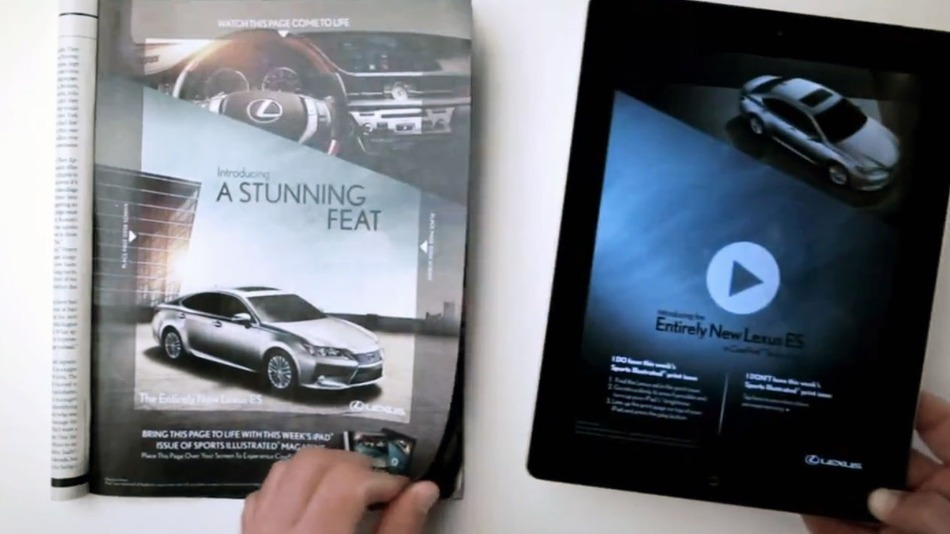
\includegraphics[scale=.50]{chapter2.tex/lexus}
\caption{Interactive Print Advertisement}
\end{center}
\end{figure}

Car manufacturers had already engaged a potential audience by creating game-like experiences where consumers could design their own vehicle and examine it in 3D. Cross-media experiences such as this, transform print into something new.

On October 5, 2012, \emph{Entertainment Weekly} placed a smartphone inside its print magazine. The phone contained a digital ad running video and live tweets  \citep{ulanoff:2013ma}. 

\begin{figure}
\begin{center}
 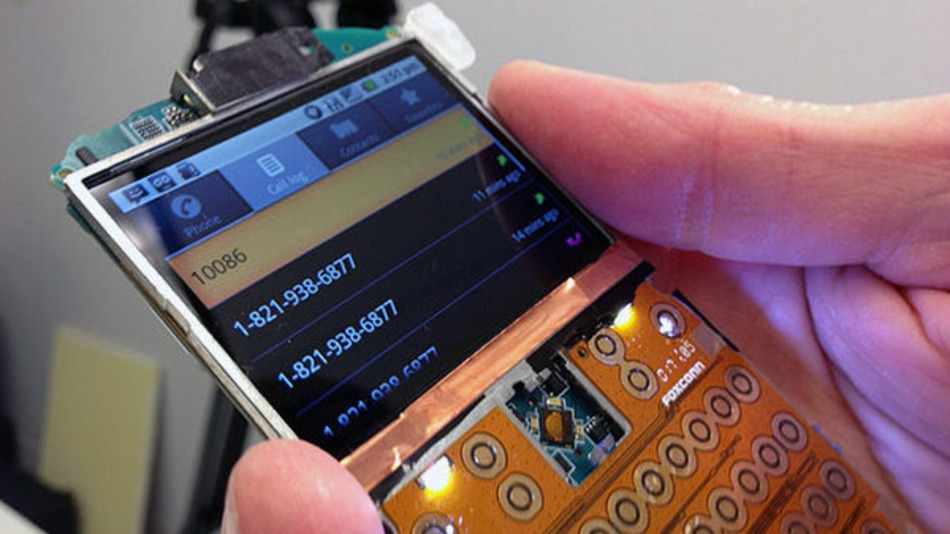
\includegraphics[scale=.50]{chapter2.tex/smartphone}
\caption{Print-Embedded Smartphone}
\end{center}
\end{figure}

It has become easier to imagine a world where print seems fluid and magic --- as envisioned by J.K. Rowling portrays the Daily Prophet in the world of Harry Potter.

Not surprisingly, there is a strong interest by advertisers to engage over mobile platforms. Utilizing location-based coupons, the iButterfly app engages customers by gamifying  coupons.\footnote{\url{http://www.cherrypicks.com/products/ibutterfly}}  Users flick their phone to hunt virtual 3D butterflies.

While interactive advertising may appear tangential to behavioral advertising, there is a common theme underlying both: \emph{interactivity}. Behavioral advertising relies on the ability to observe users engaging in everyday activities while interactive ads provide a means for advertisers to invite consumers to engaged with brands and products.

Why should this parallel concern us? It does not seem far-fetched to imagine the content of interactive ads become more tailored to the interests and expectations of individuals. Advertisers already argue that OBA benefits the consumer by delivering a more tailored (and presumably less annoying) experience. The argument posed by advertisers is fairly simple: wouldn't you rather see advertisements about products that interest you rather than advertisements about things that do not?

Suppose that advertisers collect images of your friends and family and create facsimiles which appear in  advertisements.\footnote{FaceBook may already use your posts and personal data for advertising \citep{goel:2013nyt}. Google also includes Google user names, faces, and content in ads \citep{kelly:2013cnn}.}  In June 2013, Alessandro Acquisti spoke of the following research in progress.

\begin{quote}
Imagine that an organization has access to your list of Facebook friends, and through some kind of algorithm they can detect the two friends that you like the most. And then they create, in real time, a facial composite of these two friends. Now studies prior to ours have shown that people don't recognize any longer even themselves in facial composites, but they react to those composites in a positive manner. So next time you are looking for a certain product, and there is an ad suggesting you to buy it, it will not be just a standard spokesperson. It will be one of your friends, and you will not even know that this is happening. \citep{acquisti:2013ted}
\end{quote}

The problem is that, even with policy efforts toward transparency of collection and use, it is remarkably easy to manipulate people to behave in predictable ways. As advertisements become increasingly interactive --- and as methods for collecting and using online behavioral data become more sophisticated --- we will need to become much more attuned to ways in which this data may be used to drive behavior. 

\section{Summary}
\label{summary}

This chapter introduced the phenomenon of online behavioral advertising to include issues leading to the formation of law and policy as well as issues concerning user notice and choice --- principles espoused by policy makers and advertiser self-regulatory bodies alike. 

Two mechanisms for user control were introduced: ``do not track'' and the AdChoices advertising option icon. Both present a means for users to opt-out of behavioral advertising. Both present user interactive mechanisms of choice. And both present opportunities for manipulating behavior in subtle ways.

The remainder of this dissertation is largely concerned with the study the cause of user confusion in specific contexts. The next chapter first introduces a theoretical framework for meaning and understanding in interaction. In addition, I briefly cover previous work in the areas of graphical communication and language and advertising.

\chapter{Theoretical Framework}
\label{theoreticalframework}

Language has long played a role in successful advertising. Not surprisingly, as new media have emerged, advertisers have skillfully adapted to form. 

 \cite{Vestergaard:1985vna}  studied the language of press advertisements from 1976--1977. Though noting the contextual role of visual elements, the primary focus of their work was textual.

\begin{quote}
There is no reason to believe that TV and press advertising differ in their persuasive methods in a basic way, although an analysis of TV adverts, owing to the processual character of the TV commercial and its use of both sound and picture, requires an additional body of analytic procedures. \cite[p. 10]{Vestergaard:1985vna}
\end{quote}
\begin{sloppier}
They considered advertising as, fundamentally, a message-based, one-way communication. Though they acknowledged psychological effects of messages, textual content was seen as meaning "transfer".
\end{sloppier}

About the same time,  \cite{Geis:1982uf}  studied linguistic communication in television advertisements. He proposed that advertising discourse was better analyzed under a cooperative model of communication. Commercials both directly address viewers and also communicate indirectly by promoting products through dialogue between characters. He focused strongly on the persuasive use of language, in particular, highlighting the subtle ways in which language can be used to mis-lead consumers.

This chapter presents the notion that some user interactions associated with online behavioral advertising evoke discourse processes using mechanisms similar to those described by  \cite{Geis:1982uf}.  Furthermore, such phenomena are representative of a new sort of advertising discourse. First, I introduce the notion of pragmatics and inferential communication. Then, I describe properties of discourse under a cooperative model. Following this, I discuss the notion of discourse structure and summarize factors contributing to successful communication. Finally, I review two applications of discourse understanding upon which this dissertation builds: graphics communication and the use of language in advertising. 

\section{Pragmatics}
\label{pragmatics}


\begin{quote}
Pragmatics is the systematic study of meaning by virtue of, or dependent on, the use of language. \cite[p. 2]{Huang:2007ww}
\end{quote} 


To understand pragmatics, it's helpful to understand a bit of history in linguistic theory. The study of meaning has long been the domain of semantic theory. Moreover, semantics arose as an extension of philosophical and mathematical logic. In 1905, Bertrand Russell published a short work, ``On Denoting'', in the journal \emph{Mind} which held influence over semantics through much of the 20th century  \citep{Russell:1905tj}.  Russell argued that meaning was propositional and that most statements have truth-value. Such thinking led philosophers to devise a logic-based approach to meaning that forms the basis of formal semantics today.

In a somewhat different vein, J.L. Austin also studied language use in Philosophy. Contrary to Russell,  \cite{Austin:1975vd},  in ``How to Do Things With Words'', argued that the meaning of sentences cannot be characterized solely by truth value. In a theory of speech acts, Austin regarded utterances as performing additional functions. For example, an interrogative cannot have a value of truth or false, but is used to perform an act for the purpose of eliciting some other action (e.g., to obtain information).

\begin{sloppier}
Like Austin, \cite{Grice:1961ud} were also concerned with understanding "non-natural" meaning. They distinguished between two sorts of meaning: the kind of meaning associated with individual words of that utterance (conventional implicature) and what a speaker means by an utterance (conversational implicature). This seems a subtle distinction in the abstract, but is actually an important distinction which had great impact on the discipline now known as pragmatics.
\end{sloppier} 

\textbf{Conventional implicature} relates to the meaning inherent in the words of an utterance. For example, Grice demonstrates using the word ``but'' in the utterance ``she was poor but honest''  \cite[p. 127]{Grice:1961ud}.  What is meant literally, is ``she was poor'' and ``she was honest''. However, ``but'' \emph{implicates} a contrast between ``poor'' and ``honest'', suggesting that honesty is a trait not generally associated with poverty. He notes further that if one were to change ``but'' to ``and'', the literal meaning of the utterance would not change --- but the implication would be gone  \cite[p. 129]{Grice:1961ud}.  

 \cite{Grice:1975vw}  also identified a class of implicatures known as \textbf{conversational implicatures}. This sort of implicature is exemplified by the following example:

\begin{description}
\item Speaker A: Can you close the windows?
\item Speaker B: Sure.
\end{description}

In this example, speaker A is understood by speaker B to be making request. According to Grice, speaker B reasons that speaker A has some reason to make this utterance: it must be somehow relevant to the situation. Conversation implicatures are understood by reference to a \emph{conversational situation} and are inferred via a cooperative principle and general maxims of conversation  \cite[p. 46; covered in more depth later in this chapter]{Grice:1975vw}.  To this end, conversational implicatures also depend on conversants understanding each other's goals and intentions.

In contrast to a formal study of semantics, the discipline of pragmatics holds that the study of language must systematically study meaning \emph{in the context of use}  \citep{Huang:2007ww}.  Under this view, pragmatics is considered a component of an integrated theory of language much as phonetics, phonology, morphology, syntax, and semantics. Phenomena typically considered pragmatic include \textbf{implicature}, \textbf{presupposition}, \textbf{deixis}, and \textbf{speech acts}. 

Presuppositions share some properties of implicature. They are also derived by inference. The famous sentence ``the king of France is bald'' presupposes that there is a king of France, though this is not explicitly stated. Unlike implicature, the presupposition does not change under negation. ``the king of France is not bald'' still presupposes a king of France. 

Deictic expressions are those that make reference to some aspect of context. This context may be expressed symbolically as in ``tomorrow'', ``here'', ``you'', or ``over there'', accompanied by gesture. Deixis is a universal phenomena expressed in all languages. Deixis exists because ``a language without deictics cannot serve the communicative needs of its users as effectively and efficiently as a language which does have them''  \cite[p. 132]{Huang:2007ww}. 

Speech acts derive from Austin's theory of performatives. Under a more general theory of speech acts, speech acts follow certain conventions.  \cite{Searle:1969vw}  defined five types of (illocutionary) speech acts:

\begin{enumerate}
\item \textbf{Assertives} - speech acts which express a proposition with a truth value and play the role of asserting, claiming, reporting, etc.
\item \textbf{Directives} - speech acts which represent an attempt for the speaker to get the addressee to do something as in a question, request, command, etc.
\item \textbf{Commissives} - speech acts which commit the speaker to do something in the future as in a promise, offer, threat, etc.
\item \textbf{Expressives} - speech acts which expresses a psychological state or attitude such as praising, thanking, apologizing, etc.
\item \textbf{Declarations} - speech acts which intend to change bring about change as in a declaration, nomination, etc.
\end{enumerate} 

Functionally, speech acts express strategies for communication. While speech acts have long been considered linguistic acts \cite[][and many others]{Searle:1969vw,Levinson:1983ww}, they also have a social function.\footnote{In fact, \cite{Geis:1995vo} argued that speech acts are not linguistic acts at all --- but social acts. } In standard speech act theory, illocutionary acts are directed toward addressees. \cite{Clark:1982tg} argued, however, that such acts may also be directed toward other participants that are not addressees. Furthermore, they argued that there must be an act called an \textit{informative act} which is directed toward participants who are not addressees. Consider this excerpt from the 1998 movie, \textit{The Truman Show}, where the lead character is unaware that he is starring in a live television drama:
\begin{itemize}
\item [T:] Why do you want to have a baby with me? You can't stand me!
\item [M:] That's not true! ... Why don't you let me fix you some of this Mococoa drink, all natural cocoa beans from the upper slopes of Mount Nicaragua, no artificial sweeteners!
\item [T:] What the hell are you talking about?!? Who are you talking to?!?
\item [M:] I've tasted other cocoas, this is the best!
\end{itemize}
Truman becomes confused because he recognizes that his wife, Meryl, is directing information towards an audience while speaking with him. It's easy to see that participant roles have bearing on how we produce language in interaction. 

One of the great challenges of studying pragmatics is the use of language in social contexts. Of the three experiments in this dissertation, the first concerns the hypothesized incidence of implicature, the second deixis, and the third concerns participant roles in interaction. In Chapter 8, I suggest that these several case studies are potentially indicative that pragmatic reasoning occurs during user interaction online. As we will see, such reasoning may also lead to mis-understanding.
 

\section{Language in Interaction}
\label{languageininteraction}

While philosophy was the well-spring of pragmatics, sociology and anthropology were more concerned with interactional aspects of language. John Gumperz is widely regarded as the ``father'' of interactional sociolinguistics. He and Dell Hymes studied how situations and cultures affect meaning in social interaction  \citep{Gumperz:1982tc,Hymes:1974wr}.  In addition to how words and linguistic expressions affect meaning, they also studied how ``contextualization cues'' in prosody and register (i.e., language used in particular social settings) affect discourse. Gumperz widely influenced the perspective that inferential processes in interaction could be studied systematically in natural communicative contexts. For example, he gives examples of how microinteractions, such as the timing of prosodic and nonverbal cues, give evidence of breakdowns in conversational coordination  \citep{Gumperz:1982tc}. 

Both Gumperz and Hymes strongly referenced pioneering work of Sacks, Schegloff, and Jefferson  \citep{Schegloff:1973tg,Sacks:1974uy,Schegloff:1977tc,Jefferson:1972ta}.  This body of work itself was inspired by the work of sociologist Harold Garfinkel, who was concerned with how activities and routines in daily life inform social interaction.  \cite{Garfinkel:1967vn}  describes research conducted in the 1960s at the Los Angeles Suicide Prevention Center (SPC) and UCLA Outpatient Clinic. He asked the question, ``by what criteria are its applicants selected for treatment?''  \citep[p. 18]{Garfinkel:1967vn}.  Garfinkel's work directly inspired Sacks, Schegloff, and Jefferson to engage in a detailed analysis of conversation which revealed basic organizational features of conversation  \citep{Sacks:1974uy}.  

Their basic insight was that speakers organize contributions in discrete units analyzed as turns. Turns themselves are organized into sequences. According to Sacks, each turn adds to the context affecting what will be done or said in the next turn. Speaker's orient toward each other's turns revealing systematic processes regulating both speech acts contributions as well as mechanisms for error detection and repair  \citep{Levinson:1983ww}.  Pioneering work in conversation analysis in the tradition of ethnomethodology led to deeper understanding of how people manage conversation in interaction and how this system for management helps us to recognize error and repair it when detected. 

 \cite*{Sacks:1974uy}  suggested that ``rules'' (what we now think of patterns) governing the organization of dialogue form the basis of how people manage conversation. For example, short silences or overlap in speech affect how the next speaker in a conversation is selected. Also, prosodic and gestural cues serve as signals during the coordination of exchanges. In addition, structural features such as turn transitions play a role in the detection of error and constrains repairs in dialogue. And repair sequences themselves respect the turn-taking system  \citep{Schegloff:1977tc}. 

Herb Clark, noted cognitive psychologist from Stanford University, studies cognitive and social processes in language use. Building off sociolinguistic theory  \citep{Schegloff:1973tg,Sacks:1974uy,Clark:1989ur,Schegloff:1977tc,Jefferson:1972ta},   he developed a theory of conversation as joint action\footnote{ \begin{quote} 
Clark on Joint Acts: Conversations reflect the joint activities they coordinate. Every joint activity has participants --- the people actually taking part, who are distinct from nonparticipants (bystanders, onlookers, overhearers) --- and so do the conversations that emerge from them. The participants take particular roles, such as doctor and patient, teacher and student, or friend calling and friend called, and the roles constrain what the participants do and say. Every joint activity has public goals --- mutually agreed-upon purposes for carrying them out. The overall goal may be to exchange gossip, plan an outing, or negotiate a contract, and these have subgoals. Although some of these goals are set from the start, most get established as the participants go along. The participants also have private goal --- to be polite, not to lose face, or to finish quickly, for example --- and these, too, constrain what the participants do and say. Finally, people often engage in two or more joint activities at a time --- such as gossiping and eating dinner together --- so their conversation switches back and forth between them. \citeyearpar[p. 2744]{Clark:2001uu}
\end{quote} }  \citep{Clark:2001uu}. \cite{Clark:1989ur}  observed that basic turn construction units patterned into larger chunks of discourse they termed ``contributions''. These units are composed of a distinct presentation phase followed by an acceptance phase. Contributions form a hierarchy where every signal presented (verbal or non-verbal) belongs to the presentation phase of a contribution.

In this example from Clark, the presentation of ``how much does Norman get off -- '' ends with ``oh''.

\begin{description}
\item[Presentation Phase] \hfill \\
A. is it, how much does Norman get off --
\item[Acceptance Phase]  \hfill \\
B. pardon \\
A. how much does Norman get off \\
B. oh
\end{description}

Clark noted that the acceptance phase, generally initiated by B, offers A positive evidence that he understands by what A meant. This could be a verbal response or demonstration of some sort. When B has difficulty understanding, the acceptance phase may become prolonged.

\begin{sloppier}
\cite{Clark:1989ur} posited abstract levels of communication based on patterns of contributions. While a contribution is closed with acceptance, evidence of understanding has the properties of "upward completion" and "downward evidence". For any utterance, B may believe he is in one of four successive states of understanding.
\end{sloppier}
\begin{description}
\item[State 0.] B didn't notice that A uttered something.
\item[State 1.] B noticed that A uttered something  (but wasn't in state 2).
\item[State 2.] B correctly heard the utterance (but wasn't in state 3).
\item[State 3.] B understood what A meant by the utterance.
\end{description}

Understanding in each successive state presupposes understanding in the prior  state (unless evidence from a lower state suggests otherwise).\footnote{\citep{Clark:1996tm} proposed one final state: state 4: B considers taking up A's proposed joint project.} 

The contribution model serves as a means for adding to discourse. However, the amount of evidence required for demonstrating understanding may vary depending on the task. Task-oriented dialogues often require stronger evidence of understanding than other sorts of dialogues  \citep{Clark:1986uw}.  By the principle of least collaborative effort, people ground with as little combined effort as needed for the situation at hand  \citep{Brennan:1996ud}.  

When communicating through a different medium (e.g., phone),  \cite{Clark:2005wk}  predicted that people ground using whatever techniques are available to ground with least collaborative effort. They noted that while a hearer backchannel response such as ``okay'' may be little effort face-to-face or on the phone, it may take considerable effort when teleconferencing or in a chat. The cost of acknowledgement is higher since it may interrupt the speaker.
 
\cite{Clark:1996tm} observed that dialogue gives insight to factors contributing to successful communication.  This includes:
\begin{enumerate}
\item How speakers and listeners cooperate to exchange information;
\item How speakers design utterances to help listeners understand; and,
\item How listeners provide speakers with evidence of understanding.
\end{enumerate}
For conversations to succeed, participants \textbf{ground} what they say: they establish the mutual belief that addressees have understood the speaker well enough for current purposes \citep{Clark:1989ur}. This \textbf{Grounding Hypothesis} suggests information acquired by participants accumulates in a principled way: "each party is responsible for keeping track of what is being said, and for enabling everyone else to keep track of what is being said" \citep{Clark:2001uu}. 
\begin{quote}
With each contribution to the conversation, the current speaker presupposes the common ground already established; and all the parties, the speaker included, add what is new in that contribution to their common ground. \citep[208]{Clark:1992ty}
\end{quote}
Thus, in its broadest interpretation, this view of discourse corresponds to \textit{meaning exchange} using linguistic messages in social and cultural contexts. Importantly, speakers design their utterances taking into account their potential listeners --- listeners themselves are agents in particular roles \citep{Clark:1992ty}.


\section{Discourse}
\label{discourse}

Discourse is a term that is broadly concerned with the use of language. In it's broadest, most functional sense, discourse has been viewed as a kind of social practice  \citep{Goffman:1981tm,Hymes:1974wr,Leech:1983vf,gumperz:1972tf,Brown:1983wy}.  In interactional sociolinguistics, discourse has been studied as ``forms of talk''  \citep{Goffman:1981tm},  characterized as ritualized, or institutionalized talk across social and cultural dimensions. Such talk draws on socio-cultural knowledge governed by social norms which are shared, culturally specific aspects of interpretation  \citep{Gumperz:1982tc,Hymes:1974wr,Gumperz:1964ug}.  Discourse in this perspective is deeply interactive and contextual, acting as a mechanism or process for social exchange.

In conversation analysis, discourse is seen as structured; for example, as interactive frames or schemata such as routinized exchanges in  \cite{Goffman:1981tm}  ``replies and responses'' or  \cite*{Sacks:1974uy}  ``adjacency pairs''. The recognition of such schemata are learned and form the basis for ``co-occurrence expectations''  \citep[p. 162]{Gumperz:1982tc}.  Such conversational inferences are context-bound and conceived as preferences, maxims, or tendencies.

Discourse is also the focus of study in text analysis. ``In its most general significance, a text is a sociological event, a semiotic encounter through which the meanings that constitute the social system are exchanged''  \citep[p. 199]{Halliday:1977vj}.  Such study is concerned with phenomena relating meaning and structure beyond the bounds of a simple turn or sentence --- ``stretches of language received to be meaningful, unified, and purposive''  \citep[p. 156]{Cook:1989wu}.  This includes textual structures playing a role in cohesion, coherence, narrative, and rhetorical structure; cognitive structures such as theme-rheme, topic-focus, foreground-background, given-new, contrasts; and also, syntactic and semantic structures participating in discourse-level anaphora, presupposition, and tense.

\subsection{Discourse Continuum}
\label{discoursecontinuum}

Discourse analysis widely includes practices listed above --- interactional sociolinguistics, conversation analysis, text analysis, and pragmatics. From a cognitive perspective,  \cite{Clark:1996tm}  considers language as a form of \textbf{joint action} embodying individual and social processes. The use of language in joint activities lies on what he calls a \emph{discourse continuum}  \citep[\ref{continuum}][p. 50]{Clark:1996tm}.  


\begin{figure}
\centerline{
  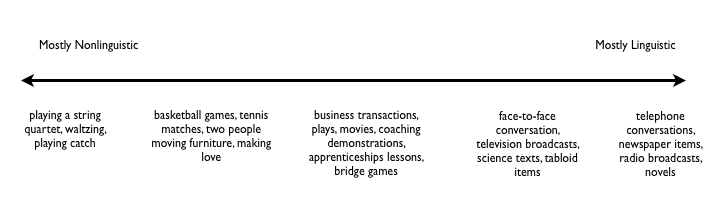
\includegraphics[scale=.75]{chapter3.tex/discourse-continuum}
  }
\caption{Discourse Continuum \citep[adapted from][]{Clark:1996tm}}
\label{continuum}
\end{figure}


To the far right, all activity is accomplished using language. Moving to the left, language is augmented by diagrams, gesture, video etc. In the middle, language is balanced by action, while further to the left, language has less of a role in the content and coordination of activity. But, according to Clark, \textbf{``if we include any signal --- any communicative act --- then language use is present across the entire discourse continuum''}   \citep[p. 51]{Clark:1996tm}.  

In this dissertation, \emph{I claim that user interface components, to include interactive graphics, can be considered as units of discourse} falling somewhat on the right side of of this scale. Undoubtedly, such components contain both graphical and textual elements, but they are also interactive, and as such, trigger patterns of thought and behavior associated with language use. Though such interaction is not strictly conversation --- since applications do not have beliefs and intentions operating in coordination with the user --- application designers model user tasks relying on the user's basic linguistic competence to interpret cues during interaction. This idea will be discussed further Chapter 8.

\subsection{Discourse Models}
\label{discoursemodels}

Ultimately, underlying language use are speaker intentions. Such intentions account for why someone can express the same concept in different ways. For example,  \cite{Donnellan:1966uv}  gave the famous example, ``Smith's murderer was insane'' as an attributive description versus referential description (e.g., ``Jones''). In his view, to say ``Smith's murderer'' is to say something about this person rather than to pick out or identify  him.\footnote{\cite{Kripke:1979ti} distinguished between these two descriptions as contrasting a semantic referent with a speaker referent.} 

But this sort of indefinite reference raises problems for a semantic analysis of reference. To account for a range of discourse phenomena such as this,  \cite{Kamp:1993wm}  proposed a theory of discourse representation which includes a representation of a \textbf{discourse model}. This structure contains a set of discourse referents (entities under discussion) and conditions which represent information that has been given about referents.

 \cite{Kamp:1993wm}  and, independently  \cite{Heim:1982wp},  made it possible to analyze chunks of discourse using a semantic analysis. But the idea of discourse models was not entirely new. ``Discourse models make explicit the structure of not of sentences but of situations as we perceive and imagine them''  \cite[p. 419]{JohnsonLaird:1983vt}.  Such models help to account for how people comprehend language. One piece of evidence given for discourse models are \textbf{bridging inferences} --- a sort of implicature by which people flesh out missing details in discourse  \citep{Clark:2002vz}. \cite{Stenning:2008uh} and \cite{JohnsonLaird:1989uj}  cited work from  \cite*{Bransford:1972tz}  giving experimental evidence that recalled sentences are inferences from explicitly presented material. An example used was,

\begin{itemize}
\item[(a)] Three turtles rested on a floating log and a fish swam beneath them.
\end{itemize}
Subject later confused this sentence with:
\begin{itemize}
\item[(b)] Three turtles rested on a floating log and a fish swam beneath it. 
\end{itemize}

 \cite{Bransford:1972tz}  argued that memory for language draws on the use of representations organized around referents (entities) in scenes and events. Models are updated incrementally and inferences about participants are made when needed. In this way, its possible to remember things about a discourse referent while not remembering how the information was conveyed.

The notion of direct and indirect representations made by  \cite{Stenning:1995ka}  is important. In their view, while indirect representations such as those used in language have a syntax, direct representations do not. It is the aim of a discourse model to provide a direct representation. As discourse proceeds, the discourse model is revised to accommodate new beliefs, but is also subject to revision when conflicting information arises. The notion of a discourse model has been crucial to theory in linguistics that accommodates a wide range of semantic-pragmatic phenomena to include anaphora, deixis, tense, and presupposition. Discourse models have also been applied to graphical reasoning where such representations are posited as a means to achieve efficiency in cognitive processing given constraints in working memory  \citep{Stenning:1995ka}. 

Discourse models have been formalized in semantics  \citep{Kamp:1993wm},  computational linguistics and artificial intelligence  \citep{Hobbs:1985ue,Grosz:1989wu},  cognitive science  \citep{Stenning:2002vd,JohnsonLaird:1989uj,vanDijk:1983tk}  and cognitive psychology  \citep{Clark:1996tm}.  In these models, discourse is structured to account for informational links as well as the role of context in meaning  \citep{Grosz:1986up}.  Discourse is also considered fundamentally cooperative, thus models take into account belief and attentional states of addressees  \citep{Clark:1996tm}.  Finally, such models account for the role of lexical, grammatical, and structural properties of language in pragmatic inference.

Thus, \emph{discourse processes concern how information is comprehended and produced}. This involves creating, accessing, and using discourse representations (or models)  \citep{Graesser:2012wz}. As \cite*{Graesser:2012wz}  observed, discourse processing research is multi-disciplinary encompassing linguistics, psychology, computer science, and neuroscience. Techniques used in study include corpus analysis, mathematical and statistical modeling, ``on-line'' experimentation (e.g., during comprehension), and brain imaging. 

While discourse researchers have busily been studying new forms of communication --- some broadcast-oriented, such as lectures, radio \slash  podcast, print advertising --- others more interactive, such as those found in computer-mediated discourse (e.g., discussion forums, chat, microblogging, and blogging), little attention has been yet afforded to direct interaction with media such as multimedia advertisements. To do so would necessitate analyzing the coordinated use of both graphics and language. The next section of this chapter specifically looks at work associated with graphics and diagram understanding and the role of discourse models as a unified representation for textual and graphical elements.

\section{Applications}
\label{applications}

In this section, I consider two applications of discourse understanding relevant to claims made in this dissertation: graphics communication and advertising language. The first summarizes work claiming that implicatures may be understood in graphical diagrams. The second describes how advertisers make use of language to persuade and manipulate. Both are relevant to a discussion of how people may be manipulated in user interaction in the context of online behavioral advertising.

\subsection{Graphics Communication}
\label{graphicscommunication}

There is reason to think that messages produced by graphical user interfaces may be interpreted under the same inferential model of communication as language.  \cite{Stenning:2006wu}  define graphics as ``planar displays of information that use the distribution of shapes, patterns, and annotations and the relation between them to convey information''  \cite[p. 476]{Stenning:2006wu}.  In simpler terms, graphics use spatial relations, in addition to text labels, to convey meaning. Good examples are maps, tables, and charts. 

 \cite{Stenning:2006wu}  note that their definition also fits textual language. While text on a page is essentially organized linearly, there is an abstract syntactic structure which encodes meaning relations between parts -- thus mapping to space indirectly. Graphics, on the other hand, encode meaning in a direct spatial representation. 

Diagrams are limited in the number of dimensions they can use to map relations. This might include icon shape, color, order, etc. Each dimension is directly mapped to a semantic representation. Phrases, words, morphemes, and phonemes, on the other hand, pack many relations across multiple abstract levels, each syntactic relation having a distinct semantic representation.

 \cite{Tversky:2004wj,Tversky:2010ww}  summarized a body of psychological experimentation demonstrating parallels between graphics, gesture, and language. Shared cognitive principles allow for mapping between visual and verbal modes in a number of domains. She described work from  \cite{Denis:1997}  in which route directions and maps could both be decomposed into a series of segments. Each segment was described to have four elements: a start point, orientation, progression, and end point. For example, ``exit the Central Square station, turn left, go down Mass Avenue until you come to Cafe Centro''  \cite[p. 146]{Tversky:2004wj}.  The correspondence between both descriptive textual elements and graphical depictive elements suggest a common, underlying conceptual structure.

Tversky argued that such meanings of schematic visual forms (glyphs and other devices) both convey and constrain meaning  \cite{Tversky:2010ww}.  Glyphs combine into complex diagrams using domain-specific syntax rules in a manner similar to linguistic structures  \citep{Tversky:1999ta}.  Similarly,  \cite{Tversky:2010ww}  noted that glyphs may be used to abstractly represent a variety of concepts such as objects, collections, relations, and processes. Such representations participate in cognitive processes such as ``inference, analogy, generalization, transfer, and insight''  \citep[p. 2]{Tversky:2010ww}. 

Though graphics and language differ in expressiveness and information packaging, they can both be studied using pragmatic theory  \citep{Stenning:2002vd,Stenning:1995ka}. \cite{JohnsonLaird:1989uj}  described the machinery by which linguistic representations (logical syllogisms expressed graphically) can be used to construct and update a  mental model\footnote{Mental models are considered equivalent to discourse models \citep{JohnsonLaird:1980uf}. However, the term "discourse model" is preferred here as it is has been more widely adopted by researchers in the academic traditions discussed.}. 

A syllogism consists of two premises followed by a conclusion as in:

\begin{enumerate}
\item All A are B
\item All B are C
\item Therefore, all A are C
\end{enumerate}

Syllogisms are defined from a narrow set of ``moods'': All A are B, No A are B, Some A are not B  \citep{Khemlani:2012ii}.  It is also possible to make constructions that look like syllogisms such as:

\begin{enumerate}
\item In some cases when I go out, I am not in company.
\item Every time I am very happy I am in company.
\item Therefore, in some cases when I go out, I am not very happy. \cite[p. 1]{Khemlani:2012ii}
\end{enumerate}

What makes example above different is the application of \emph{quantifiers} (e.g., more than) and \emph{determiners} (all, every, some, etc.) and over more complex objects such as sets and events. Contrast this with the limited logic of ``all'', ``some'', and ``no'' in a syllogism. The construction seems very similar --- but its meaning potentially much more complex.

Such constructions are interesting to study because they are informative of how people reason and also amenable to online (realtime) experimentation. Interestingly, not only does content affect reasoning (e.g., people are more likely to accept a believable conclusion than unbelievable) but when encountering such constructions, people are also highly susceptible to pragmatic inference  \citep{Khemlani:2012ii}.  

Another interesting property is that they can be expressed graphically. In fact, such graphics are effective methods for teaching deductive logic  \citep{Stenning:1995ka}.  Euler diagrams, such as  \autoref{euler}  helps aid comprehension by providing a more direct representation of the syllogism at the top of this section.


\begin{figure}
\centerline{
  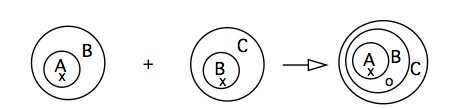
\includegraphics[scale=.75]{chapter3.tex/syllogism}
  }
\caption{Graphical Syllogism \citep{Stenning:1995ka}}
\label{euler}
\end{figure}


 \cite{JohnsonLaird:2007ua}  argued that, in fact, people do not learn as children a ``mental logic''. They acquire understanding of lexical structures (including connectives, quantifiers, relation terms, etc.) and use these to construct models of premises. Inferential schemas and the ability to calculate semantic validity are what's necessary for logical reasoning.

While  \cite{Oberlander:1995vv}  argued for graphical implicature in the use of graphical notations for computer-assisted design in electronics, I argue that implicature can also be found in user interfaces. This makes them particularly amenable for deliberate manipulation. The next section focuses on how advertisers use language to persuade and manipulate. The use of graphics and language for advertising have been a rich area of study, though not yet in the context of interaction.

\subsection{Advertising and Language}
\label{advertisingandlanguage}


\cite{Cook:2001up} argued that advertising is, in itself, a form of discourse.  Though previous linguistic analysis tackled such discourse by focusing primarily on textual or verbal elements, he argues that other contextual elements should not be divorced from analysis.  This is in contrast to earlier attempts to study language use in advertising where linguistic analysis had focused primarily on textual content and style \citep{Leech:1966wr,Vestergaard:1985vna}.

As \cite{Geis:1982uf} observed in his study of the language of television advertising,\footnote{Geis's \citeyearpar{Geis:1982uf} study is based on the analysis of 800 commercials made between 1978 and 1981.} the goal of commercial advertising is to get consumers to buy. \cite{Geis:1982uf} focuses especially on the arguments that advertisers use in order to persuade users to buy products. By persuasion, Geis meant the process by which a message is taken up such that the recipient is convinced of its truth or is moved to act. He distinguished this from manipulation in that \textit{persuasion involves conscious evaluation by the recipient on the source message and manipulation does not}.

Not surprisingly, language can and does play an important role in the process of persuasive advertising. Advertisers use language to convey messages, but also for more subtle purposes. As Geis noted, language performs a role in getting viewer attention, supporting arguments used to persuade, and playing a role in facilitating consumer memory on the desirability of the product or service \cite[p. 23]{Geis:1982uf}.

Central to how advertisers use language for persuasion is the notion of implication. Advertisers are bound legally not to use deception in order to sell. \cite{Brandt:2013un} observed that the FTC took a strong position on "misleading advertising" during the 1970s. During this time, it recognized the role of cognitive research in demonstrating how consumer world knowledge might interact with ads to form false beliefs. Thus the FTC began to rely on behavioral research to determine whether an ad was misleading. In fact, there are many ways ads can be misleading without direct assertion. 

\begin{quote}
Probably a fundamental reason has been the more subtle forms of deception that the FTC has become desirous of controlling. 'Was it deceptive for Wonder Bread (ITT, 1973) to claim it is high in nutrition when the claim is literally true yet might imply falsely that the quality is unique to itself? Did the name "Safety Champion" (Firestone, 19721 Firestone, 1973) imply that a tire is perfectly safe, or that it is safer than other tires? \citep[p. 5]{Brandt:2013un}
\end{quote}

\subsubsection{Persuasion Through Implicature}
Geis adopted a Gricean position on advertising precisely because advertisers often persuade through the use of implicatures. He gives the following example,
\begin{itemize}
\item[(a)] Wartsoff contains Vivaline and you know that Vivaline removes warts instantly. \citep[p. 26]{Geis:1982uf}
\end{itemize}
The implication is that Wartsoff removes warts instantly. An unsuspecting consumer might reason that since the advertiser used the verb "know", there must be solid evidence that Vivaline removes warts instantly.

Geis focused on three sorts of implicatures: 1) conventional implicatures; 2) theoretical implicatures (those which depend on listener belief for validity); and, 3) conversational implicatures.  

The Wartsoff statement is an example of a conventional (embedded) implicature by the use of "know". Because the word "know" has been used, it is implicated that there is good evidence supporting that Vivaline removes warts instantly.

A theoretical implicature, on the other hand, is given by the example:
\begin{itemize}
\item[(b)] Choosy mothers choose Jif. \citep[p. 48]{Geis:1982uf}
\end{itemize}
The implication is that if a mother doesn't choose Jif, she isn't a good mother.

Finally, the following is an example of a conversation implicatures:
\begin{itemize}
\item[(c)] We're building a reputation, not resting on one. \citep[p. 50]{Geis:1982uf} citing an ad in Newsweek, 2/6/1978
\end{itemize}

Here the implication is that Ramada Inn has a leading competitor that rests on its reputation. But, of course, this is not explicitly said. However, because resting on a reputation was mentioned --- it must in some way be relevant to the listener.

To back off just a bit, \cite{Grice:1975vz} proposed that language is governed by the Cooperative Principle. According to Grice, the cooperative use of language in conversation appears to follow certain maxims, or rules. In particular,

\begin{description}
\item \textbf{Quantity:} Say no more and no less than is necessary.
\item \textbf{Quality:} Say what you believe to be true; do not say what lacks adequate evidence.
\item \textbf{Relation:} Say what is appropriate at the appropriate time; be relevant.
\item \textbf{Manner:} Be clear; be brief; be perspicuous; avoid obscure expressions.
\end{description}

Grice hypothesized that such maxims generate implicatures. In particular, he focused on examples of when such maxims were "flouted" such that the listener is expected to understand the message, despite violation of  conversational rules.

In fact, we flout these maxims on a regular basis. Examples of obvious flouting are in the use of irony and metaphor. 
\begin{itemize}
\item[(d)] Brilliant! (Exclaimed after tripping)
\item[(e)] Great weather we're having. (After sudden clap of thunder)
\item[(f)] Those two are peas in a pod.
\end{itemize}
\cite{Tanaka:1999tq} noted the use of metaphors and puns in advertisement.
\begin{itemize}
\item[(g)] What makes a shy girl get Intimate (Intimate, Revlon) \citep[p.104]{Tanaka:1999tq}
\end{itemize}
She suggested that the reader is expected to get and reject:
\begin{itemize}
\item[(h)] What makes a shy girl become intimate.
\end{itemize}
in favor of:
\begin{itemize}
\item[(i)] What makes a shy girl buy Intimate perfume.
\end{itemize}
Likely, such use of implicature is intended to attract attention and intrigue and not to mislead. 

\cite{Geis:1982uf} argued that while advertisers may be held accountable for misleading the public through conventional and theoretical implicature, this may not the case for conversational implicature.
\begin{itemize}
\item[(j)] Wet feet? LOOK OUT FOR A COLD --- Gargle with LISTERINE QUICK \cite[p. 49]{Geis:1982uf}
\end{itemize}
In the example above, attributed to \cite{clark1944advertising}, Listerine is conversationally implicated by the Maxim of Relevance. In fact, Geis mentions that after 40 years of advertising in this manner, the advertisers was finally compelled by the FTC to add the disclaimer:

\begin{quote}
While Listerine will not help prevent colds or sore throats or lessen their severity, Listerine's strong formula keeps your breath clean for hours --- it kills the germs that can cause bad breath.
\end{quote}

In this disclaimer, the advertiser still exploits a conventional implication by stating that Listerine does not help prevent colds. As Geis notes, conventional implicatures are perceptually less salient than assertions though, nonetheless, implicate a relation.


 \subsubsection{Overt and Covert Communication} 

 \cite{Sperber:1986uk}  argued that there is reason to recognize a distinction between an \emph{informative intention} and \emph{communicative intention}. The first makes ``manifest or more manifest to the audience a set of assumptions.''  \citep[p. 58]{Sperber:1986uk}  The second makes it `` mutually manifest to audience and communicator that the communicator has this informative intention.''  \citep[p. 61]{Sperber:1986uk} 

\begin{sloppier}
In \textbf{ostensive-inferential communication}, as described by \cite{Sperber:1986uk}, an ostensive act by the communicator is intended to be recognized. Thus, a pointing gesture intends to draw attention to some aspect of the physical context that the communicator thinks worthy of attention. 
\end{sloppier}

In  \cite{Sperber:1986uk}  view, \textbf{relevance} is the key to human cognition. Humans pay attention to things most relevant. A communicator that \emph{manipulates context} has an affect over what is perceived more or less relevant. This means that the communicator needs to be aware of what contextual information is accessible to the addressee in order affect the process of comprehension.

From this point-of-view, ostensive communication is successful if the hearer is able to ``recover the speaker's informative intention''. \textbf{Covert communication}, on the other hand, is described as:

\begin{quote}
A case of communication where the intention of the speaker is to alter the cognitive environment of the hearer, i.e., to make a set of assumptions more manifest to her, without making this intuition mutually manifest. \citep[as quoted in Tanaka 1994, p. 41]{Bencherif:1987up}
\end{quote}

 \cite{Tanaka:1999tq}  argued that covert communication is used in advertising for two main purposes. First, to make the addressee forget that he is trying to sell her something. Second, to ``avoid taking responsibility for the social consequences of certain implications arising from advertisements''  \citep[p. 44]{Tanaka:1999tq}.  Tanaka follows with a number of examples centered on the use of sexual imagery and captioning to promote products which are not obviously sexual. For example, she shows an image from a watch ad where there is a background image of a man and woman in swimsuits embracing. A subtle caption indicates: ``designed to perform.'' Though the ad overtly communicates that these watches are designed to perform well in aquatic sports, there are strong suggestive overtones in the image clearly implicating sexual performance.

As  \cite{Sperber:1986uk}  noted, a large difference between Grice's approach (to include neo-Gricean theories proposed by  \citealp{Horn:2006va} and \citealp{Levinson:2000ud})  and theirs  (i.e., \textbf{Relevance Theory})  is that Grice's principle and maxims are norms that all people are expected to know and recognize. Implicatures are recognized and understood as violation of these known norms. By contrast, Relevance Theory is general to the point that people don't need to recognize or know anything. All that is necessary is that each ostensively communicated act have a presumption of relevance.

As advertising has adapted to new forms of media, so has the means by which advertisers harness language. Though researchers have made study of press and television advertising, little attention has been paid to behavioral and interactive advertising (with the exception of privacy notices). One can already imagine ads where people who look like one's friends recommend products used by those friends. More subtle are ad interactions, hidden in plain sight, that alter one's beliefs in fleeting moments in time. It would not be surprising to find that advertisers exploit cognitive tendencies in inferential communication activated during the course interaction.

\section{Conclusion}
\label{conclusion}

On the basis of reviewed literature, I propose that there are gaps in knowledge that have not yet been addressed: first, that interaction with graphical user interfaces involve discourse processes affecting comprehension; and second, that online behavioral advertising participates in a new form of advertising discourse where user's beliefs are affected during the course of interaction. I show that this view gives insight into communication errors difficult to explain otherwise.

\begin{sloppier}
The next chapter describes my research program and method for data collection and analysis. To follow in Chapters 5 through 7, I focus on specific sorts of pragmatic mis-understandings in the domain of online behavioral advertising.  Each time a user opens a web browser and interacts with a website, that user is challenged to make decisions about what to communicate --- and to whom --- in an environment where commercial actors actively encourage disclosure. Because discourse comprehension relies much on inference, manipulation may subtly take advantage of automatic processes such that the user is unaware of the potential for mis-understanding. Though \cite{Kahneman:1984td} and others have observed that small changes in context affect judgement and decision-making, there is considerably less research on how small changes in context affect understanding during the course of interaction in decision-making tasks. This is the topic under discussion in the remainder of this dissertation.
\end{sloppier}


\chapter{Method}
\label{method}

In this chapter, I outline a general research program and associated substantive and experimental hypotheses. Following, I describe the use of Amazon Mechanical Turk for the collection of behavioral data, general procedure followed, and summary of the population sample observed.

\section{Research Program}
\label{researchprogram}

There is little question that interaction with computers change what we know and believe. Usability has long been concerned with the fit between user ``mental model'' and the design of user interfaces. Typically, such studies include the use of qualitative research techniques such as cognitive walk-throughs, eye-tracking, and card sorting. Such studies are often task-oriented and situated to address the use of specific products.

Dan Saffer, in his book \emph{Microinteractions}  \citeyearpar{Saffer:2013wn},  touches upon user interaction with user interface components, or features, that perform only one small task. For instance, a login screen embodies a self-contained interaction that may be quite small, but extremely important for user experience. This microinteraction has a clear start and end. As Saffer notes, some triggers to enter a microinteraction are user-initiated, and some may be system-initiated. Regardless, I believe there is a clear parallel to conversational discourse discussed in the previous chapter: users exchange information interactively.

This dissertation examines several microinteraction in the domain of online behavioral advertising. Of particular interest are phenomena relating to user confusion in the context of online interaction. 

The substantive hypothesis for questions asked in this dissertation is that \emph{some user confusion stemming from online behavioral advertising is caused by error in discourse understanding}. I contend that by regarding user interaction with graphical user interfaces as a form of discourse, we can account for some sorts of user confusion that may be difficult to see or may otherwise go un-noticed.

The next section summarizes specific research hypotheses for this dissertation. The research approach used to examine these hypotheses is \emph{randomized experimentatal}. The purpose for adopting such an approach is to determine causality for some sorts of user confusion. Each research hypothesis is paired to some aspect of discourse theory. Therefore, Chapters 5, 6, and 7 more fully motivate the connection between theory and practice prior to a presentation of results.

\section{Design of Experiments}
\label{designofexperiments}

The substantive hypothesis (user confusion stems from errors in discourse understanding) implies a set of research hypotheses, which in turn imply individual study hypotheses.

\begin{description}
\item[Research hypothesis 1:] \hfill \\ 
Graphical user interfaces have properties comparable to other forms of linguistic communication. 

\item[Research hypothesis 2:] \hfill \\
Graphical user interfaces can cause users to make faulty pragmatic inferences.

\item[Research hypothesis 3:] \hfill \\
A pragmatic inference derived while interacting with a graphical user interface may be affected when given immediate and direct feedback.
\end{description}

Each of the three sets of experiments described in Chapters 5-7 support one more more of the research hypotheses above. Specific research manipulations  are described below. The number in the left column refers to the experiment number.
\\
\\
\textbf{Research manipulation} (by experimental condition):
\begin{description}
\item[1A:]  \hspace{6pt}Suppose that pragmatic inference only occurs in linguistic (text or speech) interaction. A graphical user interface is used in the experimental condition whereas text is used in the control condition.
\item[1B:]  \hspace{6pt}Suppose that system feedback adds information to a situation model. Feedback is used in the experimental condition while none in the control condition.
\item[2A:]  \hspace{6pt}Suppose images and icons are objects that are both indexical. Images and icons are combined such that contrastive relations exist in the experimental condition while none exists in the control condition.
\item[2B:]  \hspace{6pt}Suppose advertising images are implicitly indexical. Explicit indexical element appears in the experimental condition while none exists in the control condition. 
\item[3:]  \hspace{12pt}Suppose that a user designs utterances taking into account potential listeners. Listener roles are explicit in the experimental condition while implied in the control condition.
\end{description}

Finally, the table below summarizes experimental designs. Each should be considered a pilot study. That is, experiments described are new and there are no other results against which to compare. The goal is to apply difference statistics to determine whether the variables described are independent (null hypothesis) or dependent. A relation between variables indicates some degree of predictiveness and causality. We can use information about causality to guide, or motivate, a strategy for reducing the possibility of miscommunication.

%% LyX 2.0.6 created this file.  For more info, see http://www.lyx.org/.
%% Do not edit unless you really know what you are doing.
%\documentclass[english]{article}
%\usepackage[T1]{fontenc}
%\usepackage[latin9]{inputenc}

%\makeatletter

%%%%%%%%%%%%%%%%%%%%%%%%%%%%%% LyX specific LaTeX commands.
%% Because html converters don't know tabularnewline
%\providecommand{\tabularnewline}{\\}

%\makeatother

%\usepackage{babel}
%\begin{document}
%B%
%\begin{table}
%\begin{center}
\begin{longtable}{l p{10cm}}
\caption{Experiment Design} \\
1A & 2x2x2 between group posttest-only design where the control group is
presented with a set of textual expressions and asked to answer
questions about their meaning. Treatment groups are presented with either textual expressions or a dialog box expressing the same set of choices and asked the same
questions. Independent Variables: Modality, Deontic force, Attitude
toward privacy. Dependent Variable: Pragmatic implicature\tabularnewline
\hline 
1B & Between group posttest-only design where two groups are presented
with a cookie banner and later asked about whether or not they believe
the website placed \textquotedbl{}cookies\textquotedbl{} in their
browser. The treatment group is presented with feedback about the
consequence of their action / non-action following presentation of
the banner. Independent Variable: Feedback. Dependent Variable: Pragmatic
implicature.\tabularnewline
\hline 
2A & Between group posttest-only design where five groups are presented
an advertisement in the context of a webpage and asked to identify
hyperlinks. Treatment groups are presented an advertisement with embedded
image icons at four levels (known icon + different company, unknown icon, known call-to-action (CTA), ``DAA opt-out icon'') while the control group is presented with an embedded image from the same company as the advertiser. Independent
Variable: Icon type. Dependent Variable: Indexicality of icon. \tabularnewline
\hline 
2B & Between groups posttest-only design where three groups are presented
an advertisement in the context of a webpage and asked to identify
hyperlinks. Treatment groups are presented an advertisement at two
levels (iconic CTA, textual CTA) while the control group is presented
with an advertisement with no CTA. Independent Variable: Modality
of CTA. Dependent Variable: Click target.\tabularnewline
\hline 
3 & Between group repeated measures posttest-only design where a control
group is asked to respond to a survey containing questions relating
to activities (using questions drawn from \cite*{Acquisti:2012tp}; embarrassing, socially / ethically questionable, illegal). Participants
are notified in a privacy statement that there may be ad trackers
on the site. The treatment group receives exactly the same notification
and survey. However, tracker presence is indicated in a visual display
throughout the participant's session. Independent Variable: Visual
presence. Dependent Variable: Propensity to respond in the affirmative
to engaging in specific behaviors.\tabularnewline
\hline 
\end{longtable}
%\end{center}
%\end{table}
%\end{document}


Of course, not every usability problem needs be tested using experimental methods. But there are two good reasons to do so here:

\begin{sloppier}
\begin{enumerate}
\item No causality has yet been determined for presumed cases of mis-communication studied here. In fact, it may not even be apparent that there is a problem at all.
\item Though linguistic theory offers explanation for the sort of miscommunication described in experiments here, there are no earlier studies with which to compare. This dissertation intends to make such a relation clear and provide a path for future exploration. 
\end{enumerate}
\end{sloppier}

Each of the research hypotheses above has bearing on current practice in online behavioral advertising as represented in technical specifications of existing or proposed standards. Though self-regulatory bodies for OBA suggest that specific principles are adhered, effectiveness is in question. Marketing advocates affirm that self-regulatory practices are effective  \citep{AdChoicesOurExpe:2012ux}.  However, research studies by policy advocates  \citep[e.g.,][]{Komanduri:2012wo,Mayer:2012wt}  have raised issues of industry non-compliance. Even if compliance were universal, usability studies have uncovered inadequacies in terms of communicative efficacy  \citep{Leon:2012vu,Ur:2012ws,Hastak:2010vf}.  The benefit of the approach in this dissertation is the ability to test technical specifications, and ascertain effectiveness in context. 

One of the particular challenges of the randomized experimental approach is the need for a larger number of participants than one might expect from a traditional usability experiment. Increasingly, psychologists and linguists have come to rely on the large pool of volunteers available via the Amazon Mechanical Turk (AMT) crowdsourcing platform. The next section addresses both advantages and disadvantages of AMT for experimentation. Characteristics of the user sample studied have particular bearing on the research validity of experiments presented in this thesis.


\section[Mechanical Turk]{Mechanical Turk as a Platform for Human Intelligence Tasks}
\label{mechanicalturkasaplatformforhumanintelligencetasks}


The original Mechanical Turk constructed in the 18th century was a hoax. In all appearance, he was a mechanical man dressed in an turban and robe, seated behind a large cabinet. Despite being mechanical, he played chess like no other machine could. Of course, unknown to most at the time, inside the cabinet was a tiny space where a real human played the game by controlling the automaton's arms on the chessboard. 

By contrast, Amazon's Mechanical Turk (AMT) is no hoax. From a simple command line interface, requester's can create ``human intelligence tasks'' and farm them out to a sea of workers. Within seconds, a task may be accepted, completed, and remunerated without the requester ever knowing or communicating with the invisible worker. AMT shares a simple design concept with the original Turk: a human is in the machine. The idea is a ``job posting board'' where human intelligence is needed. Any of a variety of ``Human Intelligence Tasks'' (HITs) can be posted along with small monetary rewards ranging from cents to dollars. AMT is a prototypical example of crowdsourcing --- outsourcing to a large, undefined community of people (i.e., crowd).

\subsection{The AMT Marketplace}
\label{theamtmarketplace}

In 2006, Wired magazine published the influential \emph{The Rise of Crowdsourcing}  \citep{Howe:2006uj},  which tells the story of the rise of the amateur on the web. Highlighted, is the example of a stock photo site iStockphoto which created a marketplace for amateur photographers. Professional grade camera technology at affordable prices combined with the ability to upload content to the Internet, search and categorization, and micro-payments changed the market for photographers and photo purchasers. Over the last decade, the power of many users over distributed networks has changed the world. Today, FaceBook and eBay could not exist without the contributions of their users.

The irony is, of course, that by engaging in the creation of user-generated content on the web, people have become part of the machine. This has led to the well-known technology humanist Jaron Lanier to rail against the de-humanization of the web. His position is --- to design applications that treat humans as machines devalues both people and content ``making ourselves into idiots''  \citep{Lanier:2006wb}.  Lanier particularly dislikes Wikipedia which creates a false sense of authority behind information by removing any connection between the real author of the information as well as a subjective context for the interpretation of content  \citep{Lanier:2010ud}. 

Nevertheless, crowdsourcing has become a viable economic model on the web. More than a million workers login to crowdsourcing platforms to complete short tasks for pay-per-task compensation  \citep{Munro:2011tm}.  And who is the invisible worker? As reported on The Mechanical Turk Blog in August of 2012, ``turkers'' comprise a workforce approximately 500,000 persons (at any one time) across 190 countries. In an analysis of the AMT marketplace over multiple studies,  \cite{Mason:2011cl}  report that the majority of turkers reside in the United States or India and tend more likely to be female (55\%) with a median average age of 30 and, on average, earning 30K per year. According to Ipeirotis  \citeyearpar{Ipeirotis:2010tt,Ipeirotis:2010jo},  workers in the US are more likely to use AMT as a secondary source of income while those in India use it as a primary source of income. Workers are self-selected on the marketplace, working for cash payments in US dollars and Indian rupees. All studies agree that workers are represented across a wide range of ages, ethnicities, countries, languages and income.

The AMT marketplace has been active since 2005. Among the most well-known documented instances of use, turkers were asked to help search through sections of satellite imagery to flag images with anomalies. The hope was that turkers might be able to help pinpoint the 2007 crash site of aviator Steve Fossett. This event so permeated the media at the time, I signed up to become a turker in order to participate. In the end, Fossett was not found in the region examined by turkers. In fact, there was some criticism toward the use of turkers for annotating satellite imagery. With little understanding of what constitutes anomaly in satellite imagery, the usefulness of generated leads were considered by some to be questionable.

Since then, AMT has been used for a variety of tasks, some of which call for specific skill or expertise, such as knowledge of a foreign language. More common are tasks that involve transcription, rating, editing, and image annotation. The AMT website provides a basic web interface for loading HITs, though it is also possible for requesters to direct workers to an external website or directly embed that website as an iframe on the AMT site.

\begin{figure}
\centerline{
  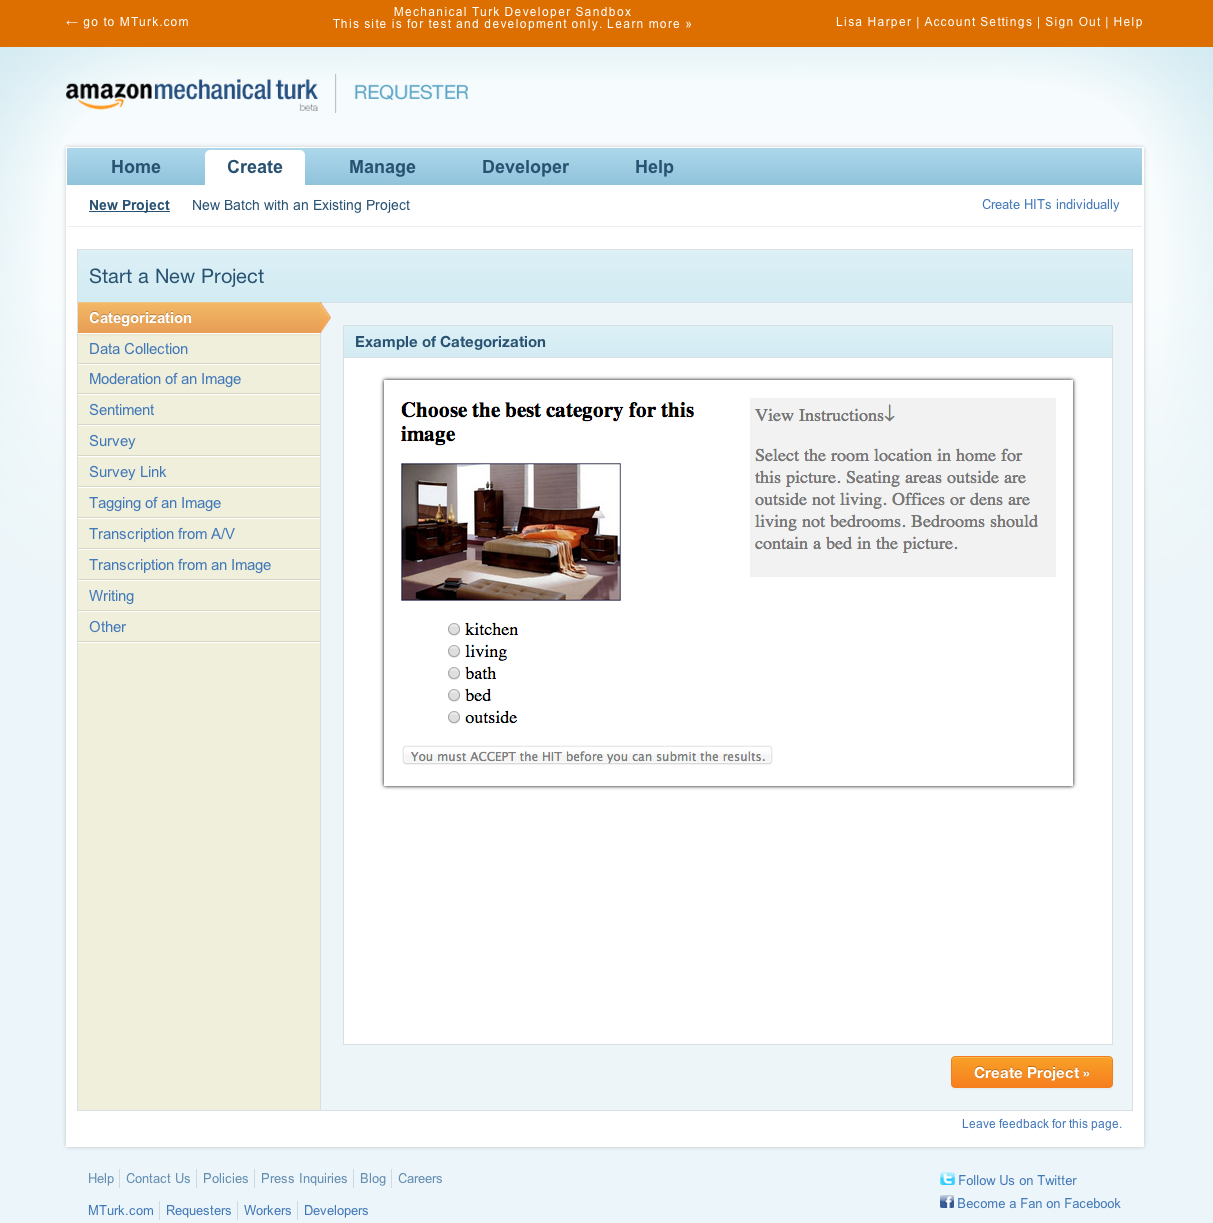
\includegraphics[scale=.5]{chapter4.tex/amt-creator}
  }
\caption{AMT Requester Website}
\label{requestor}
\end{figure}

Workers themselves comprise a community that interact on public forums, such as \emph{Turker Nation}, and through networks such as Twitter. Once on the AMT website, workers track their earnings (managed by Amazon), status (HIT success), qualifications, and the ever revolving database of available tasks.  \autoref{requestor}  is a screengrab taken from the AMT developer sandbox, a place for requesters to test tasks before deploying on the AMT website.

\begin{figure}
\centerline{
  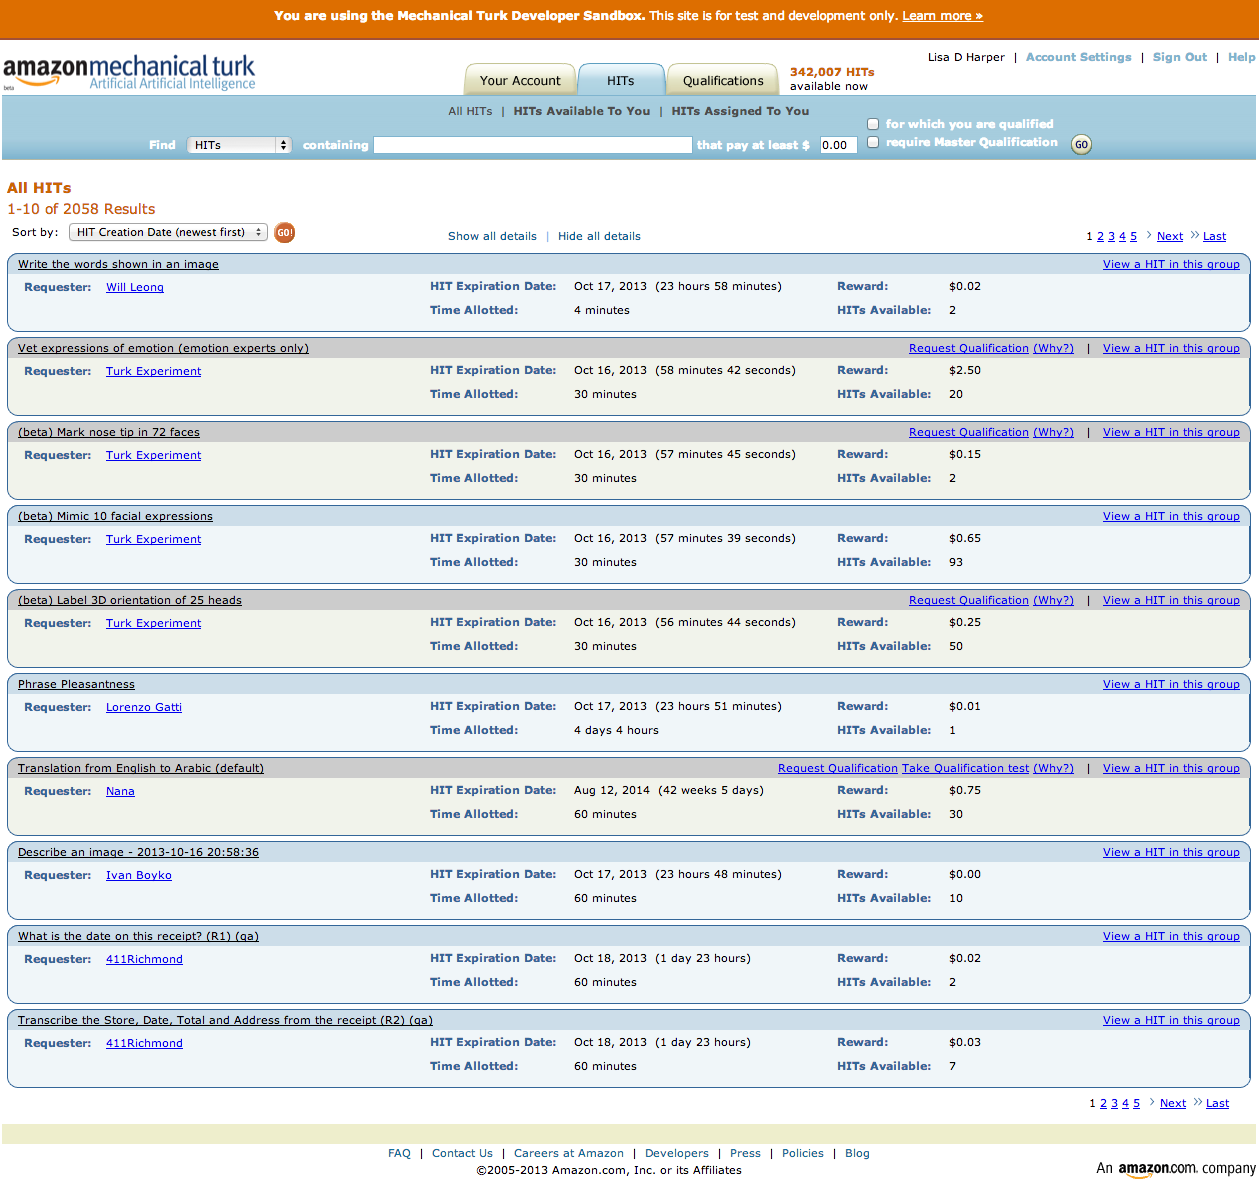
\includegraphics[scale=.5]{chapter4.tex/worker-hits}
  }
\caption{AMT Worker HITs}
\label{worker}
\end{figure}


Requesters define the task, number of tasks available, payment, qualification, and expiration date. Requesters must provide a validated US bank account and address in order to initiate tasks. Some basic worker qualification types are provided by Amazon out-of-the-box: worker HIT success and demographic region are commonly used by requesters. However, requesters also use qualifications as a mechanism for training workers. By requiring workers to ``train'' and go through testing, workers with special skills may be utilized in future tasks.

Because the worker success metric is often used as a filter for ensuring higher quality work --- and as a means for obtaining higher paid HITS --- workers take care to protect their rating. This means that requesters are also held accountable in their dealings with workers, via informal ratings over social media channels. Though some HITs may be paid automatically, it is fairly common for requesters to do quality control before accepting HITs. HIT rejection has negative consequences and is not taken lightly by the turkers.

There are a number of obvious advantages to using AMT. The workforce is roughly half a million strong and available around the clock. They represent a wide demographic range, many quite well educated. Amazon manages and automates payments and ensures the pool of workers abides by its terms of use.  \cite{Mason:2011cl}  observed that, for experimental research, a key advantage is faster iteration between hypothesis formulation and testing. However, there exists a number of real concerns and issues with crowdsourced experimentation. These are discussed below.

\subsection{General Concerns with the Use of AMT for Experimental Research}
\label{generalconcernswiththeuseofamtforexperimentalresearch}

First, and foremost, AMT is an Internet-based platform.  \cite{Reips:2006bm}  noted advantages as well as disadvantages to experimentation over the Internet (relative to the first four bullet points below). However, there are also number of other issues particular to Mechanical Turk.

\begin{enumerate}
\item \textbf{User Fraud.} There is the possibility of worker "gaming" through multiple submissions. The Turk Requester's Blog \footnote{\url{http://turkrequesters.blogspot.com/2013/01/the-reasons-why-amazon-mechanical-turk.html}} gives an example from the Romanian Mturk Forum, in which on every page (on a total of more than 300), are discussions of how to break Amazon's terms of service. As a result, Amazon adjusted their policy to an invitation-only registration for International workers \citep{Chiarella:2013vz}.
\item \textbf{Self-Selection.} Users self-select by reviewing titles, payment, time expected, and instructions. Unless controlled, users are generally able to preview eternal websites (or embedded iframes) to decide whether they wish to accept a given HIT. 
\item \textbf{Drop-outs.} AMT workers have the ability to return or abandon HITs without affecting their reputation. However, requester's don't automatically see which workers accept --- though don't complete --- assignments, so its difficult to gauge dropouts. 
\item \textbf{Mis-communication.} Reduced communication between requesters and workers may mean that directions are not well understood or followed. This can be difficult to detect and debug.

\item \textbf{Screening.} Amazon provides no general mechanism for screening aside from a general mechanism for filtering via qualifications. Of note, is the need to screen for demographic criteria and prior participation. This study has the particular need for the latter: excluding workers who have participated in one experiment from participating in another.  The mechanism that AMT provides is exclusion by assignment:  once a worker has accepted an assignment, that particular assignment is no longer available. For example, Experiment 2A of this dissertation required at least 300 subjects. Once a worker accepted this HIT the other 299 assignments were no longer available. But, without cross-experimental controls, it would be possible for some worker to accept a HIT from a closely related experiment, potentially biasing results.
\begin{sloppier}
\item \textbf{Compensation.} The very fact that AMT is fee-based places obligation on both the requester and worker. \cite{Mason:2009dr} investigated the relationship between compensation and performance in two experiments on AMT. They observed no interaction between difficulty of task and compensation on performance. They also found that increasing compensation alone did not improve accuracy. But how workers were paid (pay-per-word, pay-per-puzzle) did have an impact on output and accuracy. 
\end{sloppier}
While it is common for workers to accept tasks for pennies each, some workers find by working many low paying tasks in quick succession, they are able to earn close to minimum wage.\footnote{See discussion at \url{http://mturkforum.com/showthread.php?2744-How-much-do-you-earn-per-hour}, for example.} More typically they earn much less \citep{Paolacci:2010ws}. Though most workers appear attracted by the earnings potential, others participate for reasons such as boredom, fun, curiosity, and even education \citep{Behrend:2011dx}.

The studies in this dissertation limit participation to workers with a high HIT acceptance rate. From discussion on turker forums and blogs (e.g., \textit{Turker Nation}, \textit{mTurk Forum}, and \textit{Turkkit-Reddit}), its clear that these workers expect to be paid more than other workers. And many take this work quite seriously. 

\item \textbf{Quality and Reliability.} Beyond recruiting from the most reliable workers available, how much should quality be of concern? From prior crowdsourcing experiments on Amazon Mechanical Turk (AMT), quality is a valid concern \citep{CallisonBurch:2010vk,gormley-EtAl:2010:MTURK}. In a study of translation tasks, researchers consistently receive poor and noisy translations including blank annotations, misspellings, copy-pasting of machine translations, and downright cheating \citep{Ambati:2010ud}. Having workflows for the filtering of noisy data has proven vital in this environment. However, it is feasible to filter noisy judgements of non-experts depending on the task: in an image annotation task \cite{Nowak:2010gt} found that, while agreement between experts and non-experts varies depending on the measure used, its influence on image ranking as a whole, is minimal. Other sorts of studies echo this finding including labeling text with emotion \citep{Snow:2008wo}, search relevance judgements \citep{Alonso:2009vya}, and more.

\item \textbf{Presentation Consistency.} All Internet experiments conducted in the wild suffer the need for exceptional attention to cross-browser effects and robust services. If the experiment relies on everyone being able to see stimuli at the same resolution and in the same manner, then both scripts and screens need to be tested carefully, both across platforms and browsers. Furthermore, hosted services require reliable access by hundreds simultaneously --- and with little risk of downtime.

\item \textbf{Anonymity.} Finally, though we would like to believe that the human in the machine is anonymous, reality differs. It is estimated that 50\% of workers have been linked to public Amazon user profiles \citep{Lease:2013vq}. This means that Amazon worker Ids are essentially PII. And, in fact, many workers are not blind to this.
\begin{sloppier}
\item \textbf{The "Superturker".} Legal scholar Dan Kahan warns particularly of a side-effect of prior, repeated exposure to cognitive studies on AMT \citep{kahan:2013blog}. Chandler, Mueller, and Paolacci \citeyearpar{Chandler:2013bw} note that while the probability that any one worker has seen some manipulation, there is a population of "superturkers" (prolific workers) who are significantly more likely to end up in studies. Pooling 16,408 HITs in 132 unique studies, they found that HITs were completed by 7498 unique workers. The top 10\% of prolific workers completed 41\% of total HITs. On a positive note, \cite{Chandler:2013bw} note that these turkers are less likely to be multi-tasking and more likely to be available for follow-up studies such as required for longitudinal research. On the negative side, these workers are much more likely to have participated in cognitive tasks potentially biasing them for future cognitive tasks \citep{Chandler:2013bw}.
\end{sloppier}
\end{enumerate}


\section{General Procedure}
\label{generalprocedure}

Each experiment in this dissertation was delivered over the Internet in a web browser. Subjects (AMT workers) were randomly assigned to groups per study design. Experiments were implemented within a Qualtrics ( \url{http://qualtrics.com} ) survey using supplementary, custom JavaScript\slash HTML\slash CSS code that I wrote, as needed. Surveys were accessible via an HTTPS encrypted iframe on the AMT website ( \url{https://www.mturk.com}). 

In order to participate, AMT workers selected my HIT from a worker queue  (\autoref{worker}).  Three base qualifications were stipulated:

\begin{sloppier}
\begin{itemize}
\item workers must be 18 years or older (provided by the Amazon Mechanical Turk Terms of Service in \autoref{amazon});
\item workers must be physically located in the United States; and,
\item Workers must have a HIT success rate of 90\% or better. 
\end{itemize}
\end{sloppier}

The AMT API provided for qualification criteria such as geographic region and HIT success rate. By specifying these as requirements, Amazon automatically matched eligible workers to my ``surveys''. A sample assignment (Experiment 1A) is provided in  \autoref{assignment}. 

Using AMT command line tools, I tested each experiment in the AMT sandbox before deploying to AMT. Requesters can monitor assignment progress, approve or reject workers, download results, and assign bonuses from their dashboard. I tested assignments in several browsers both on on a Mac and Windows PC to ensure functionality and appearance were consistent. Following successful tests, I pushed assignments to AMT. 

Workers who selected one of my HITS were told they would be participating in either a language study, user interface study, image annotation study, or ethics survey, depending on the experiment. Because these were all studies of language use, workers were expected to have basic \emph{linguistic competence} in English. It was assumed that if they were on the Internet capable of responding to a request to participate in an online experiment, and residing in the United States, they had adequate competence in English. However, I also provided a demographic survey question targeting fluency level, if the subject was not a native speaker of English.

\begin{sloppier}
Each experimental design was deployed as a single Qualtrics survey. Qualtrics provides for sophisticated functionality such as survey flow, block randomization, display and question logic, and a JavaScript application programming interface (API). Several of my surveys required hand-coded instrumentation not provided by Qualtrics. I  discuss instrumentation in the methods section of each experiment described.
\end{sloppier}

Because I conducted multiple, related experiments simultaneously, exposure to one experiment potentially disqualified a worker from other experiments. For example, Experiment 1A has a potential priming effect on the topic of Internet privacy that could potentially bias that same worker in Experiment 1B. In such cases, I included a message on the preview that said something like, ``please don't accept this HIT if you have previously participated in an experiment with a blue rectangle.'' As reinforcement, I checked each worker on acceptance of consent against a database of prior workers. If a worker had already participated in a closely related experiment, a message was presented to that worker to please return the HIT. Then they were prohibited from further access. Eve so, it was still possible for a single worker to participate in more than one experiment. For example, if a worker signed up for Experiment 1B, they were allowed to also sign up for 2B. 

In each experiment, workers previewed basic instructions  (\autoref{instructions})  before selecting the HIT. I inserted custom code to prevent participants from advancing beyond this screen until the HIT had been accepted. In order to proceed, the worker must have clicked ``Accept HIT''.


\begin{figure}
\centerline{
  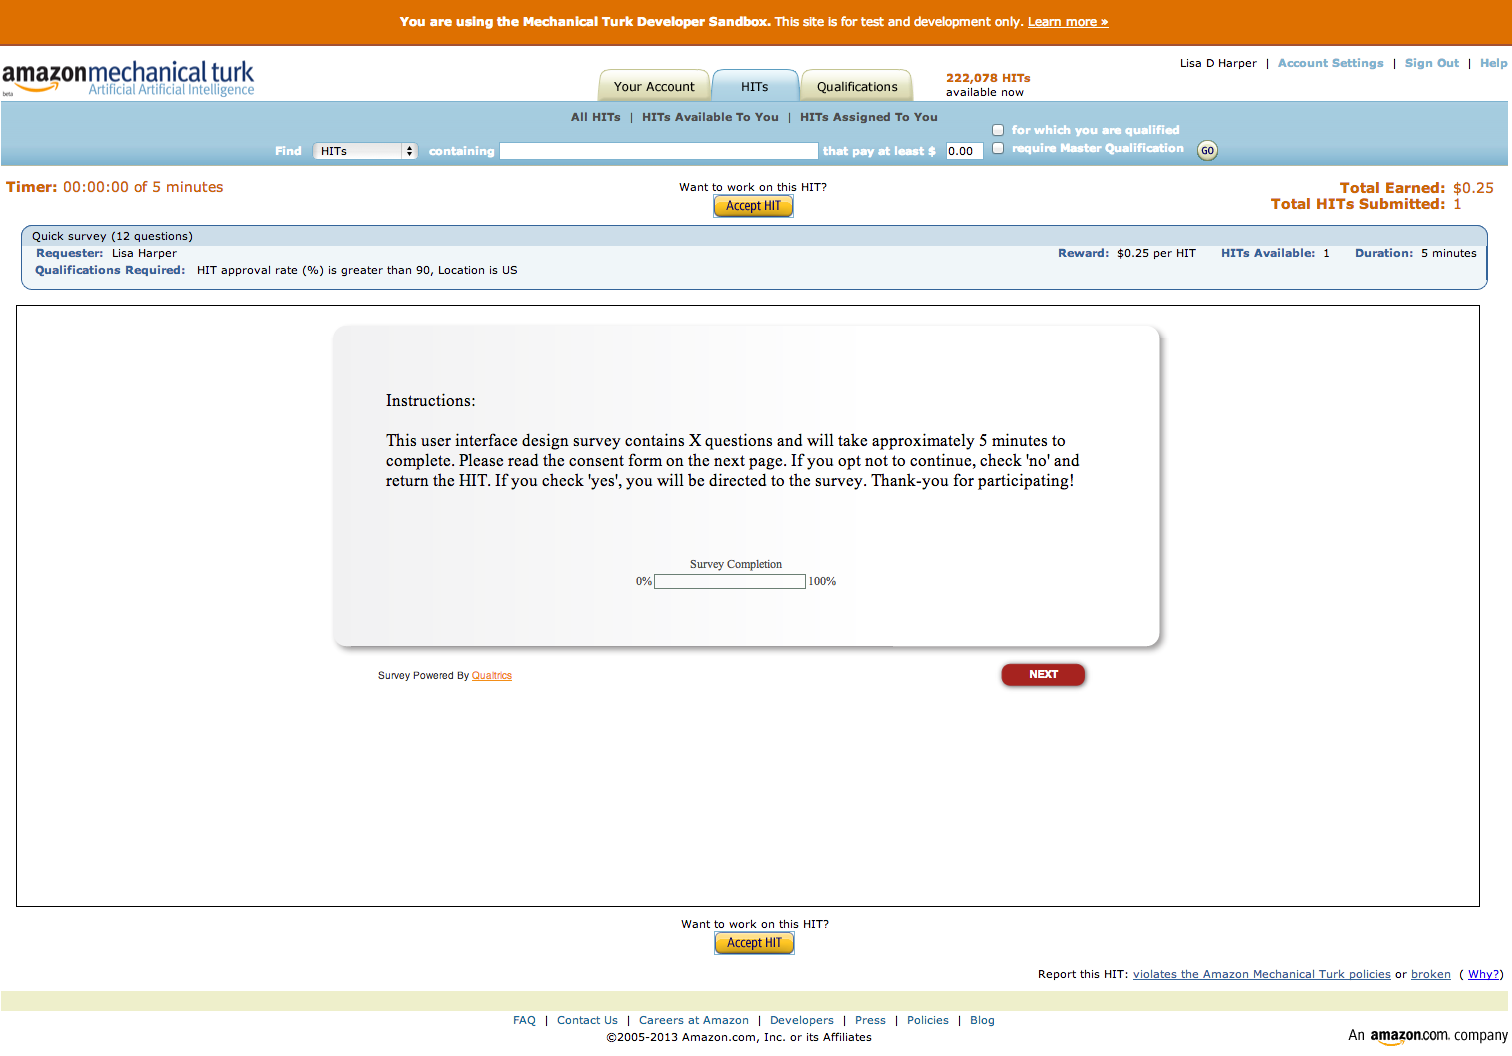
\includegraphics[scale=.4]{chapter4.tex/instructions}
  }
\caption{Participant Instructions (Experiment Three)}
\label{instructions}
\end{figure}


After clicking ``next'', a consent form was displayed (see  \autoref{consent}).  Again, in order to continue, the participant must have selected ``yes'' to continue.

General experiment flow is depicted below  (\autoref{flow}). 


\begin{figure}
\centerline{
  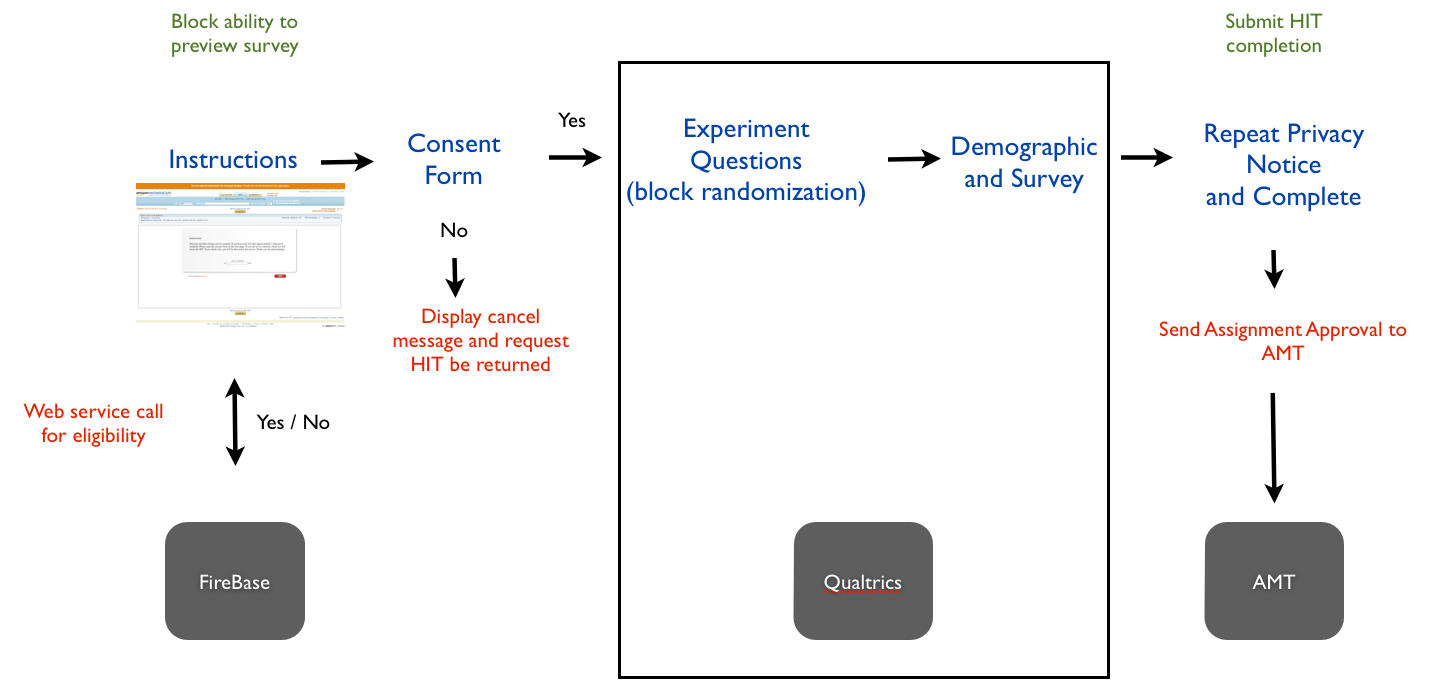
\includegraphics[scale=.25]{chapter4.tex/expflow}
  }
\caption{Experiment Flow}
\label{flow}
\end{figure}


At the completion of each survey, I configured assignments to automatically approve HITS so that Amazon would pay the worker immediately. Experiments were designed to take approximately three minutes to complete. I offered 15 cents for most. While it was also possible to manually review results before approving HITs, I decided this was not necessary for any of the studies included here since workers were recruited from those with known high performance. I did, however, manually assign random dollar bonuses after assignment completion.

\section{Data Storage and Privacy}
\label{datastorageandprivacy}

Data was stored in three places  (\autoref{data-storage}): AMT, Qualtrics, and FireBase.  AMT stored a list of workerIds for each experiment, Qualtrics stored survey data (but no workerIds), and FireBase was used to store a list of worker hashes (but no data or workerIds).

\begin{table}
\caption[Data Captured]{Data Captured}
\label{data-storage}
\centering
\begin{tabular}{cp{7cm}}
\toprule
Stored & Type of Data\tabularnewline
\hline 
Amazon Server \medskip{} & WorkerId, AssignmentId, HitId, Accept / Reject, Fees paid\tabularnewline
Qualtrics Server \medskip{}  
 & Random number identifier, Experiment data\tabularnewline
FireBase Server\medskip{}
 & Hash of workerIds for each experiment\tabularnewline
\end{tabular}
\end{table}

There was no connection between AMT and Qualtrics except for URL-encoded data passed to and from the Qualtrics server:

\begin{itemize}
\item On acceptance of a HIT, Amazon passed Qualtrics an AssignmentId, HitId, and WorkerId. 
\item On completion of the HIT, Qualtrics sent back to Amazon the AssignmentId. 
\end{itemize}

Survey data was not stored on Amazon's servers nor was participant identity accessible to Qualtrics via the AMT API. Because AMT does not offer ``verified'' user profiles, users can lie about their demographic group to qualify for a study. However, given the relative anonymity of the system, most appear to be honest  \citep{Ipeirotis:2010jo}.  

The Firebase service listed above was required only to disqualify workers from participating in certain experiment combinations. To safeguard identity, my code on Qualtrics converted the AMT WorkerId to a 32-bit hash and passed this hash to the Firebase service. New prospective workerIds were hashed and compared with the hash list on the Firebase service. Hashing is uni-directional, thus it is not possible to recover the original WorkerId from a hash list alone. 

On Qualtrics, the WorkerId was discarded and replaced with a random number identifier. WorkerId was treated as Personally Identifiable Information (PII) and de-linked from the data such that it would not be possible to re-link workerIDs to experiment results. Furthermore, though Qualtrics retains IP address data by default, I turned this, and other browser identifiers, off for these experiments. Because no identifying questions were asked, nor was IP address collected, all experiment data collected is fully anonymized. 

The next section addresses characteristics of the population sampled.

\section{Population Sample}
\label{populationsample}

The first and third columns of the table in  \autoref{survey-response}  summarize questionnaire responses across the five studies described in Chapters 5 - 7. Of the 1158 subjects who took the demographic survey, 84\% were unique, with 16\% duplication due to participation in more than one experiment. This was possible, depending on the order in which workers accepted tasks. For example, if a worker accepted a HIT in Experiment 3, that same worker was later still eligible for any of the other experiments. However, once participating in Experiment 1B, he or she would have been no longer eligible to participate further.

Demographics are comparable to those published in other studies  \citep{Ross:2010jm,Ipeirotis:2010tt,Mason:2011cl}, though the sample I collected was skewed more toward males.  Of 1158 subjects, 73\% were under 35, 53\% male, 73\% caucasian, 97\% English speaking, 86\% having at least some college, and 53\% making under 30,000 per year. The profile drawn here is from a set of workers with a 90\% or better HIT acceptance rate and from the United States.

In September of 2011,  \cite{McDonald:2011uv}  conducted a user survey on AMT to study the differences between what users expect ``Do Not Track'' to mean versus DNT definitions under debate. At the time, DNT was very new. They studied 304 participants limiting participation to the United States. 81\% had never heard of DNT.

Though I did not use those exact questions in my survey, in October of 2013, 91\% reportedly knew what a tracking cookie is. 73\% admitted to using browser plugins for privacy protection and more than half to configuring their browsers to ``opt-out''. However, despite that AMT workers are much more knowledgeable than two years ago, most still do not realize that DNT, as specified by advertisers, is limited to not showing targeted advertisements: information is still collected, stored, and used.

In an older study (not on AMT),  \cite{Acquisti:2005hv}  found a correlation between concern for privacy and income. Those with higher incomes were generally more concerned with privacy. However, this may have correlated more strongly with knowledge than income. They noted that their sample particularly lacked knowledge about technological or legal forms of privacy protection.

\section{Validity}
\label{validity}

Discussed below are three aspects of validity for studies using Mechanical Turk: internal, external, and construct validity. Questions of statistical validity are addressed in the results sections of experiments.

\subsection{Internal Validity}
\label{internalvalidity}

Internal validity concerns the equivalence between groups and the control of extraneous variables. Other behavioral experiments utilizing AMT  \citep{Crump:2013fn}  have suggested that the pool of available workers is sufficiently representative and large such that random assignments consistently produce results equivalent to those produced in carefully controlled laboratory settings. Furthermore, it is possible to conduct experiments where workers may are not aware that they are in an experiment (one source of experimental bias). Also, Paolacci et al.  \citep{Paolacci:2010ws}  found that retention was particularly high on AMT, compared to other pools compared (university student population and Internet boards). However, they noted that, unlike student populations, turker membership is organic and workers may be potentially available for years. This particularly highlights the need to track responses across experiments.

More insidious to internal validity may be the effects of payment itself. Two effects of \emph{volunteer bias} are of particular concern are: 1) effect of informed consent; and 2) effects of obligation incurred by accepting a HIT and, as as result, payment for services.  \cite{Rush:1978tw}  found difference between unpaid volunteers and paid subjects in a selective attention task. Unpaid volunteers were found to commit fewer omission errors than paid subjects.

Another potential threat to internal validity is the control of the subject environment. Mentioned previously, was the problem of ensuring all conditions are presented consistently across browser types and monitor sizes. In addition, there is no way to control what sorts of environmental factors may be present: workers may be participating in multiple tasks, watching television, or be distracted in a myriad of ways.

To address these concerns, I took the following precautions:

\begin{enumerate}
\item using custom code, I limited participation across conditions where prior exposure to privacy questions was potentially biasing; and,
\item to the extent possible, I sandbox tested --- not just code consistency, but visual consistency across platforms and browsers.
\end{enumerate}


\subsection{External Validity}
\label{externalvalidity}

One important aspect of external validity is whether AMT workers are representative of the desired population as a whole. The experiments described in this dissertation rely on basic linguistic competency. For this purpose, native language competency is of concern. Mechanical Turk appears representative of the U.S. population as a subject pool from the perspective of gender, race, and education. Previous studies  \citep{Behrend:2011dx,Buhrmester:2010ur}  find that turkers are slightly more representative of U.S. population statistics than are standard Internet samples. They are also significantly more diverse that university samples. 

The population sample participating in studies described here may, however, differ from the general Internet population in other ways. Turkers polled seemed surprisingly knowledgeable of privacy issues. This indicates that experimental results, in some cases, may not be representative of a more general population.

\subsection{Construct Validity}
\label{constructvalidity}

To large extent, construct validity is a property of each individual experiment. However, the experiments described in this dissertation fall into the genre of both linguistic and judgment \slash  decision-making tests. To this end, there exist other studies which are generally comparable. 

 \cite{Paolacci:2010ws}  conducted replication of traditional judgment and decision-making tasks on AMT and compared them with groups from traditional subject pools at a large University and also Internet discussion boards. Tests included the  \cite{Kahneman:1984td}  Asian disease problem,  \cite{Kahneman:1983tb}  Linda problem, and  \cite{Baron:1988ty}  Physician's problem. Their results confirm that AMT is a reliable source of experimental data in judgment and decision-making. Not only were group results similar across conditions, but the effect size for AMT was the highest. More generally, AMT has been validated as a tool for behavioral cognitive studies such as those in reaction time research (e.g., Stroop, Task-switching, Flanker tasks, etc.;  \citep{Crump:2013fn}  and recall of written information  \citep{Tietze:2009wn}. 

\begin{sloppier}
While researchers in natural language processing were among the first to utilize AMT for the collection and annotation of linguistic resources \citep{CallisonBurch:2010vk}, its adoption by theoretical linguists has been slow to develop. Traditionally, user judgments supporting theoretical claims have been weakly quantitative relying on a very small number of examples and researchers -- often limited to the authors of theoretical studies themselves. \cite*{Gibson:2011wp} demonstrate the utility of AMT for collecting linguistic behavioral judgments for acceptability of sentence / meaning pairs. \cite{Sprouse:2010dx} compares just such a task with two groups of users (AMT versus laboratory) each with 176 participants. Data collected from the two groups was deemed virtually indistinguishable.
\end{sloppier}

Finally, researchers in pragmatics (e.g., in studies of implicature) have begun not only to adopt experimental methods, but have applied these to collections on AMT  \citep[for example,][]{Stiller:2011vz,Degen:tr,Bergen:2012up}.  As noted by  \cite*{Assessingthepragma:2011ug},  pragmatic inference depends on a multitude of factors including task structure, social norms, and response elicited. Furthermore, because there are potentially so many parameters, it is difficult to systematically model interactions between linguistic form, context, and pragmatic inference. Crowdsourcing platforms make such study more tractable, though we have much yet to learn about what specific methods are most amenable. Problematic for pragmatic studies, in particular, is that the subject's knowledge of the experiment itself plays directly into context  \citep{Rosnow:1976wy}. 

\section{Summary}
\label{summary}


\begin{sloppier}
This chapter outlined a research program with the substantive hypothesis that some user confusion stemming from online behavioral advertising is caused by error in discourse understanding. I described three situations where mis-communication may occur. The first considers the possibility of pragmatic implicature in a "do not track" modal dialog, the second considers the indexicality of an icon embedded in an image-based advertisement, and the third the effect of visual presence on non-ratified participants on a web page.
\end{sloppier}


In this chapter, I also discussed related research utilizing Amazon Mechanical Turk, outlined general procedures and considerations, and described general characteristics of the population sampled.

In each of the next three chapters, after framing experimental hypotheses within the theoretical framework, I detail specifics in terms of instrumentation, collection, analysis and results.

\chapter{Study One: Modal Dialog Boxes}
\label{studyone:modaldialogboxes}

This study concerns whether people make pragmatic inferences when interacting with user interface components. Elements of language and iconic graphics integrate to communicate what seems a simple message. So simple, users may not even be aware of potential errors in communication.

\section{Motivation: Privacy as User Choice}
\label{motivation:privacyasuserchoice}

The W3C Tracking Protection Working Group (TPWG) has been working toward a ``Do Not Track'' (DNT) policy intended to allow users to signal their intent with regard to browser-based tracking. DNT is not designed as a general purpose tool for communicating privacy practices. It is intended to simply communicate a user's preference not to be tracked. 

The current Tracking Preference Expression draft specifies three possible states: DNT:1 (do not track), DNT:0 (allow tracking) and un-set. In this third case, tracking preference is not enabled. The TPWG draft posits a number of reasons for why a user agent may not have tracking preference enabled:
 
\begin{enumerate}
\item The browser user agent does not implement DNT;
\item The user has not yet expressed a specific preference; or,
\item The user has not chosen to transmit a preference.
\end{enumerate}

User preference mechanisms specified by the TPWG represent an earnest attempt to place some burden of policy implementation on browser developers rather than publishers: instead of forcing the user to make a choice for every website, the idea is that a user specifies choice in browser preferences and sets exceptions as desired. Nonetheless, some websites offer a tracking preference choice in order to comply with other international regulations, such as the EU cookie law described in Chapter 2.

\section{Choice Design Problem}
\label{choicedesignproblem}

Though the TPWG intent is to provide a machine readable preference expression mechanism and not a user interface (UI) specification, the three options above map to common UI pattern: \textbf{modeless dialog control}. 

Given this, if a user is presented with a dialog control presenting a choice between opt-in, opt-out and dismiss, what does the user believe is the consequence of choosing to dismiss?

One way to consider this problem is as a choice design problem (\autoref{cookieguard}):
\begin{enumerate}
\item If I click "allow",  I choose "allow" cookies
\item If I click "block", I choose "block" cookies
\item I can do neither ("dismiss")
\end{enumerate}

\begin{figure}
\begin{center}
 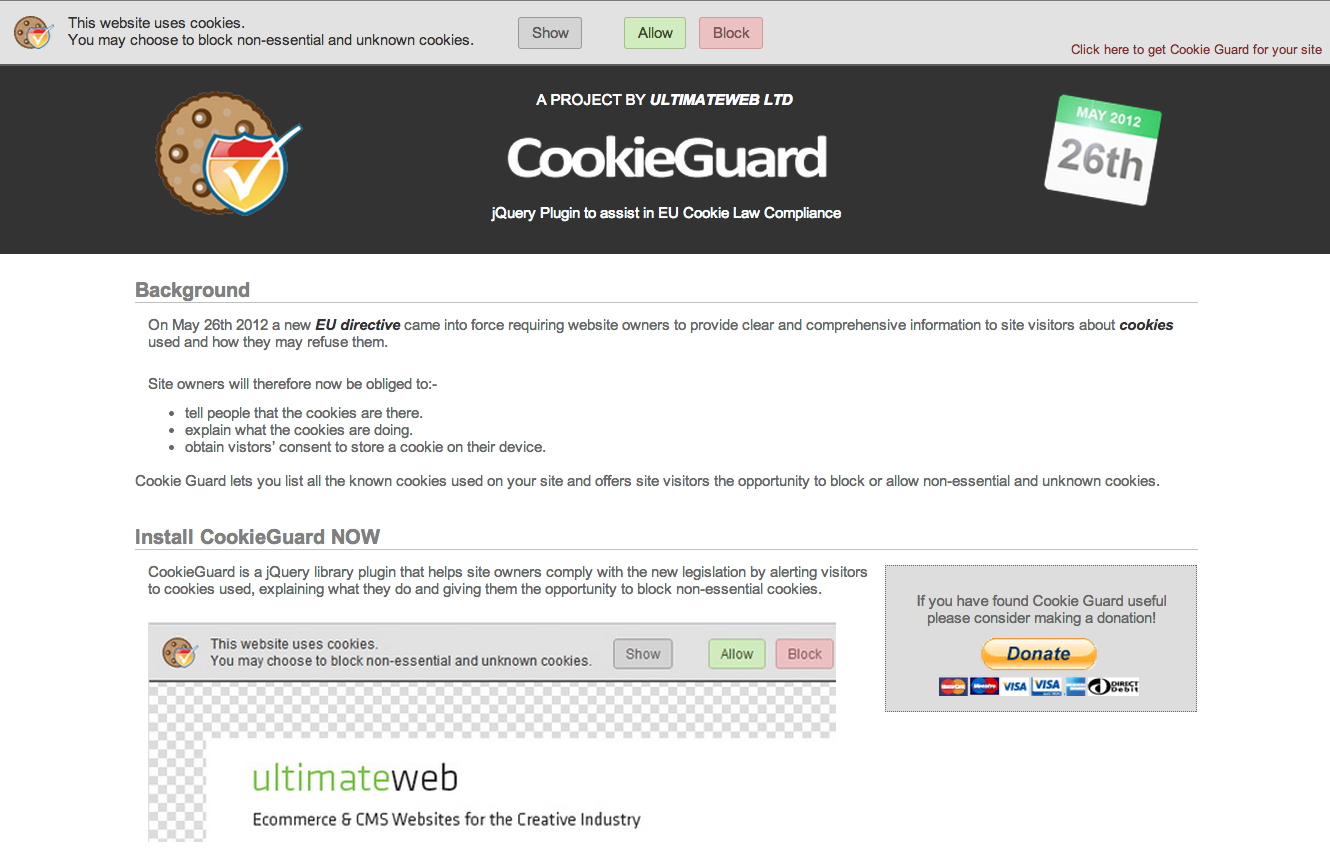
\includegraphics[scale=.25]{chapter5.tex/cookieguard}
\caption{Cookie dialog control from cookieguard.eu}
\label{cookieguard}
\end{center}
\end{figure}

Fair and unbiased choice design is a tricky problem. Default choices have a dramatic impact on user action  \citep{Johnson:2002vb}.  \emph{Heuristics and biases} theories of reasoning account for a number of different situations leading to systematic bias. Biases including loss aversion (e.g., change from status quo), framing, and evaluation of options in relation to reference points (e.g., expectation and social comparison) have been well-described by  \cite{Tversky:1981vc} and \cite{Kahneman:1984td}. 

Whether intentional or not, designers -- both standards architects and web designers -- have tremendous potential to influence choice  \citep{Thaler:2010uy}.  

\section{Forced Choice}
\label{forcedchoice}

Given that users may not understand the consequences of not making a DNT choice, one might ask why the TPWG might not specify ``forced choice.'' That is, why not force the user to make a choice? 

As described by  \citet{Dhar:2003vb},  forced choice under preference uncertainty can produce psychological discomfort  \citep[referencing work by][]{Festinger:1964ub,Lewin:1951uj,Janis:1977vx}.  They note that the no-choice alternative is an attractive way of resolving difficult choices when subjects are forced to choose. 

The study described here concerns whether users confronted with a non-forced choice dialog box understand the meaning of their choices in the context of interaction. The next section will cover related research, focusing largely on meaning and understanding.

\section{Related Research}
\label{relatedresearch}

Prior privacy research in the context of online behavioral advertising has focused on the effectiveness of communicating privacy risks to consumers  \citep{McDonald:2009td},  and confusability in user interface design  \citep{Leon:2012vu}.  Moreover, research on ``opt-in'' \slash  ``opt-out'' in the context of privacy-related decision-making has also been studied  \citep{Bellman:2001vq,Lai:2006ws}.  This body work is summarized below.

\subsection{Heuristics and Biases}
\label{heuristicsandbiases}

 \citet{Bellman:2001vq}  systematically studied the influence of question framing and defaults on consumer privacy preferences. They remarked that the decision to share private information on a site is typically on a case-by-case basis. This is particularly problematic in light of research by  \citep{Kahneman:1984td}.  who found that user behavior was susceptible to several important factors, namely the framing of options. In other words, people tend to evaluate options in relation to how a question is asked. What  \citeauthor{Bellman:2001vq}  discovered in the context of privacy preference was that framing the question as opt-out instead of opt-in affected choice. 

In  \autoref{defaults},  from  \cite{Bellman:2001vq},  134 participants were given either the first question or the second --- which are framed positively and negatively, respectively. By making opt-in the default, 96.3\% agreed to participate, while when not the default, only about half agreed to participate.


\begin{figure}
\centerline{
  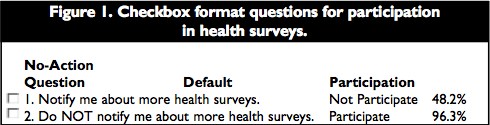
\includegraphics[scale=.5]{chapter5.tex/default2}
  }
\caption{Effect of Defaults on Participation (Image credit: \cite{Bellman:2001vq}}
\label{defaults}
\end{figure}

\begin{sloppier}
Equally interesting is that positive (e.g., "notify me about...") versus negative (e.g., "do not notify me about...") framing has an effect on participation rates. In the same task as above, but in a forced choice question format, respondents agreed to participate at a higher rate in a positive frame compared to a negative \citep{Bellman:2001vq}.
\end{sloppier}


As they further note,

\begin{quote}
Defaults and framing are likely to have even more impact when, as is often the case, the question is set in a miniature font, or answering most questions is optional, or the implications of answering are buried in a large privacy policy document. \citep[p. 25]{Bellman:2001vq}
\end{quote}

 \citet{Lai:2006ws}  extended this work by investigating the role of ``privacy concern'' on option frames. They found that that the mechanism described by  \citet{Bellman:2001vq}  had a greater effect in people who were less concerned with privacy than those who were more concerned with privacy. Thus, those with greater privacy sensitivity appeared to be less susceptible to option frames.

To date, ``opt-in'' versus ``opt-out'' in the context of dialog interaction has not been studied. However, there has been some relevant research on interaction with modal dialog, in general. In a study comparing techniques for user notification of information updates,  \citet*{Bailey:2000up}  find dialog windows to be the most most intrusive and distracting of methods compared.  \citet{Bailey:2006bp}  note that: ``when peripheral tasks interrupt the execution of primary tasks, users require from 3\% to 27\% more time to complete the tasks, commit twice the number of errors across tasks, experience from 31\% to 106\% more annoyance, and experience twice the increase in anxiety than when those same peripheral tasks are presented at the boundary between primary tasks.'' This work is particularly relevant from the perspective that people have a choice to even attend a dialog upon visiting a website.

\subsection{Pragmatic Reasoning}
\label{pragmaticreasoning}

Pragmatics is concerned with reasoning processes that go beyond conventional meaning. It is founded on the notion that communication is essentially cooperative  \citep{Grice:1975vz,Levinson:1983ww,Clark:1996tm}. 
A common pragmatic phenomenon in linguistic understanding is implicature. An implicature represents a gap between what is expressed and what is communicated. Importantly, whether an implicature is true or not, does not affect the meaning of the message itself. For example,

\begin{enumerate}
\item Harry and Sally are married.
\item Tell a friend or colleague.
\item If you mow the lawn, I'll give you five dollars. 

\end{enumerate}

In (1) the implication is that Harry and Sally are married to each other. But, if they were not, and both married to someone else, this statement would still true. (2) exemplifies implicature derived by considering ``or'' as inclusive or exclusive. (3) typifies what is known as \emph{invited inference}  \citep{Geis:1971vb}  or \emph{conditional promise} \citep{Searle:1971vx}.  In (3), hearers understand the conditional relation between getting five dollars and mowing. But they may also infer ``not to mow'' means they will ``not get five dollars.'' 

 \cite{Fillenbaum:1975tr}  showed that the obverse of a conditional promise (in the example above, ``I won't give you five dollars, if you don't mow the lawn'') was an accepted inference for 85\% of subjects tested. Invited inference in a conditional statement affects people's understanding of a situation. Such inferences contain what is known as ``deontic force''.

\subsection{Deontic Reasoning and Knowledge}
\label{deonticreasoningandknowledge}

Interestingly, arbitrary assertions such as:

\begin{quote}
If a fish is red, it has wings. \citep{Markovitz:1990pr}
\end{quote}

elicit far fewer bi-conditional interpretations (i.e., A fish has wings, if and only if it is red) than conditional promises. 

What's different? Conditional promises such as the lawn mowing example above incur some sense of social obligation. Lexical items such as ``must'' and ``may'' do, as well.

\begin{quote}
You must finish your homework before you can go out to play.
\end{quote}

Obligation is somehow implicit in the word ``must'' and its meaning is licensed by context --- if this is a mother speaking to a child, than that mother is placing constraint on her child. 

Likewise, a symbol may reflect social obligation. A stop sign is as explicit social rule and one we obey because of societal consequences. But there may also be contexts where such signs are ignored, for example, if the street is on an abandoned compound.

The meaning of assertions containing concepts of permission, obligation, and prohibition, and release (from obligation) involve what is called \emph{deontic reasoning}  \citep{Beller:2008de}.  This sort of reasoning is concerned with the relation between pragmatic knowledge (i.e., knowledge of the content of arguments) and social obligation. 

\subsection{Content Affects Reasoning}
\label{contentaffectsreasoning}

While the \emph{cooperative principle} (Grice, 1975) affects comprehension, knowledge of subject matter does, as well. If both the antecedent and consequent are closely correlated in the real world as in:

\begin{quote}
If I wear a jacket, then I put on a tie.
\end{quote}

 \citet{politzer1981differences}  found more bi-conditional interpretations for this sort of sentence than if they were not closely correlated.  \citet{marcus:1979co}  found the same for statements where the antecedent and consequent were causally related. \emph{In conditional reasoning tasks, subjects use knowledge of content to reason about the problem.}

In the experiment described in this chapter, two confounding factors are considered: \emph{deontic force} and \emph{privacy bias}. The first is invoked through the use of word traditionally seen in cookie dialog boxes --- ``allow'' \slash  ``block''. As control, I substitute the words ``on'' \slash  ``off'' which carry not implied deontic force. The second confound is knowledge and attitude towards privacy and tracking cookies. I control this factor by substituting the words ``pictures'' for cookies.

\subsection{Graphical Implicature}
\label{graphicalimplicature}

Visual context is known to influence language processing very early in the processing of language  \citep{Tanenhaus:1995tc}.  In eye-tracking tasks,  \citet{Tanenhaus:1995tc}  observed comprehension tasks on the millisecond time scale during language comprehension tasks. Initial experiments demonstrated that subjects made saccadic eye movements to objects immediately after hearing particular relevant words in instruction. Such movements are closely time-locked to linguistic objects.  \citet{Eberhard:1995fa}  found that listeners immediately integrate lexical, sub-lexical, and prosodic information in speech with information from visual context to reduce a set of referents to the intended one. 

There is relatively little empirical research directed at graphical implicatures and mixed-modal representations, in particular.  \citet{Stenning:2006wu}  and  \citet{Stenning:1995ka}  posit that diagrammatic representations may be studied using the same kinds of semantic techniques used in linguistics.  \citet{Oberlander:1995vv}  discusses the notion of \emph{graphical implicature} in diagrams while  \citet{Marks:1990wh}  discuss methods for avoiding unwanted implicatures in generating text and graphics. 

While this experiment aims to show whether pragmatic processes are in play, it makes no particular claim with regard to the processing of implicature; only that once a dialog box has been comprehended, this understanding has bearing on decision-making and belief. Furthermore, an implicature generated during understanding may not be remembered as such --- since people generally can't distinguish between assertions and implications in memory  \citep{Brewer:1977tl}  Indeed, it is likely that people are not even aware of any confusion or mis-understanding during or after comprehension.

\section{Pre-Pilot}
\label{pre-pilot}

The purpose of this pre-pilot was to assess the feasibility of conducting a larger, online pilot study. Specific questions addressed were: 1) whether the dialog was placed in such a way that subjects would likely read it; and, 2) whether subjects would consider the dialog as independent of the experiment. I needed to be confident that users would not be influenced by the environment to select a particular choice. To this end, the study was posed as a ``survey''.

\subsection{Method and Procedure}
\label{methodandprocedure}

In December 2012, 17 subjects were recruited at the University of Baltimore from university business offices. Employees and students were invited to participate in a ``10 minute survey'' in the Information Arts and Technologies usability lab in exchange for a \$5 dollar gift card. All were native English speakers who were comfortable using the Internet.

Using a Tobii T60 eye-tracker, subjects were presented with a choice banner (``This website uses cookies'') preceding a short survey on Internet privacy. The choice banner was modified from the CookGuard plugin\footnote{ \url{http://cookieguard.eu} }  \autoref{cookieguard}  designed to help website owners comply with European Union directives. 


\begin{figure}
\centerline{
  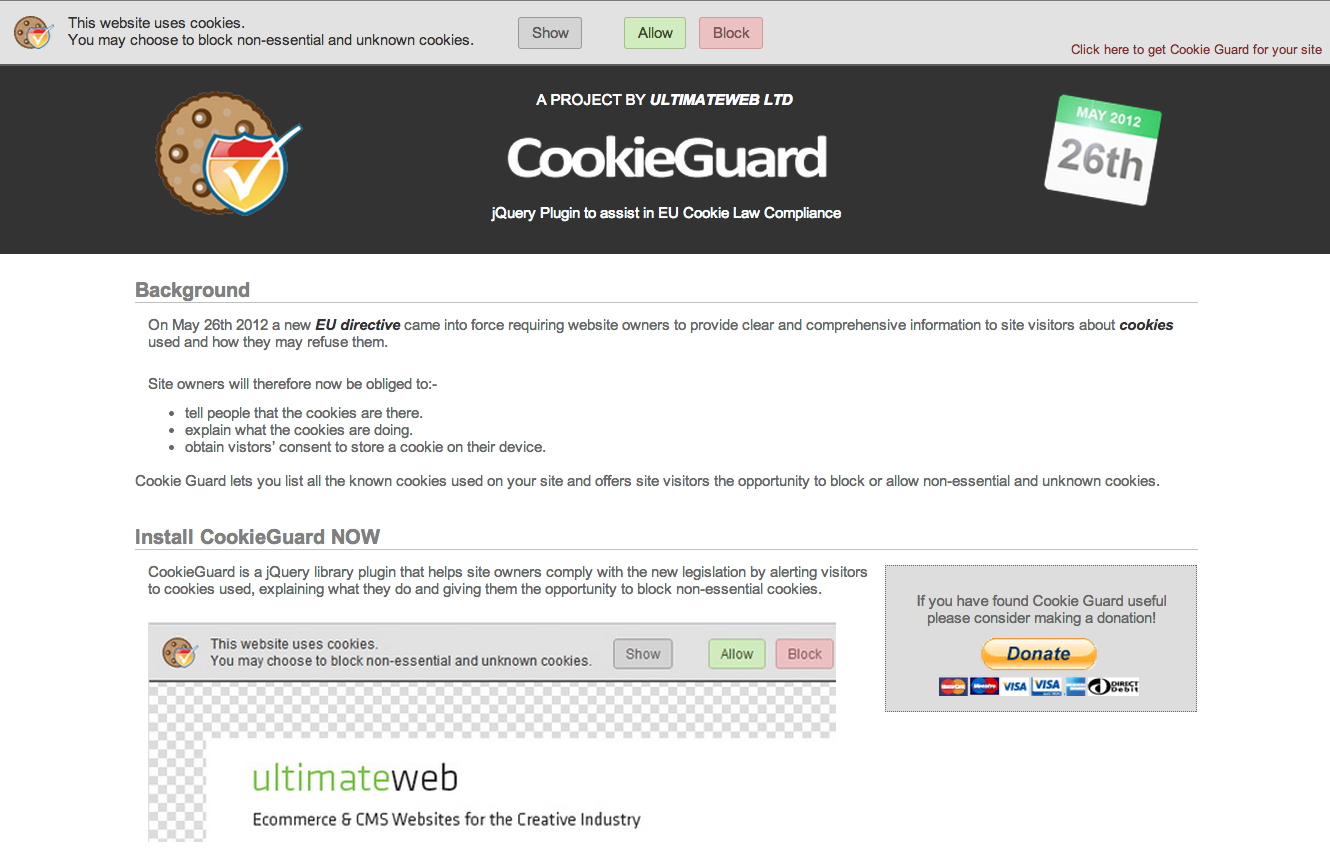
\includegraphics[scale=.25]{chapter5.tex/cookieguard}
  }
\caption{CookieGuard Website}
\label{cookieguard}
\end{figure}


A modification was made to include an ``x'' so that a third option -- ``if I click the x, I dismiss the control'' -- was explicit.


\begin{figure}
\centerline{
  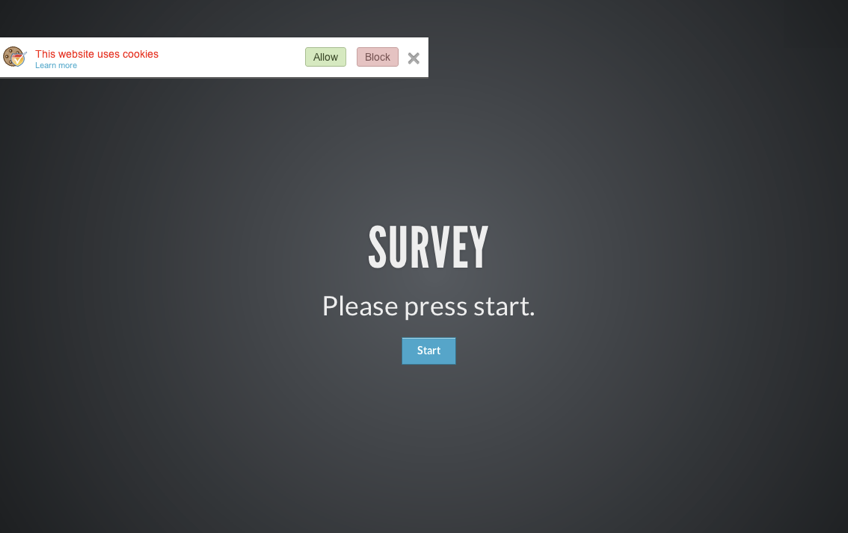
\includegraphics[scale=.3]{chapter5.tex/pilot}
  }
\caption{User Display}
\label{pilot}
\end{figure}


This banner was placed prominently on the start page of the Internet survey  \autoref{pilot}.  Generally, such banners are placed at the very top of a website, but I was concerned that subjects might not notice it there, so it was positioned it in such a way to make it more visually distinct.

\subsection{Results and Discussion}
\label{resultsanddiscussion}

Of 17 subjects, 5 did not know what browser cookies were, 14 reported that privacy was very important to them, and 15 reported that they would turn off tracking if it were easy. Notably, only 1 subject selected any option other than ``dismiss'' on the cookie banner.\footnote{Interestingly, many subjects who dismissed the cookie banner without making a choice later indicated that privacy was very important to them.} He selected ``block'' cookies because ``he didn't like cookies.'' No one clicked the provided link ``learn more''.

For the first goal of assessing likelihood that a subject would read the banner, I learned that, despite a sparsity of information on the start page, the first 9 subjects did not see the banner. For the remaining, subjects were verbally cued that there would be a cookie banner on the start page and that they could ``choose however they wanted.'' Indeed, all but one did then see and read the banner. 

The second goal was more successful. When presented the banner, subjects reported that they did not suspect that the cookie banner had anything to do with the following survey.

After presentation of the cookie banner and a number of demographic questions, subjects were asked whether they believed ad trackers were present on the site or not. 8 subjects believed that ad trackers were present while 9 did not. Of those that believed ad trackers were present, 1 subject believed that this was the case since he did not ``block'' cookies. Of the 9 that did not believe ad trackers were present, 6 believed this because they did not ``allow'' cookies. Accordingly, 7 of 17 (41\%) believed there either were or were not ad trackers on the site based on \emph{not} clicking ``allow'' or ``block'' cookies, respectively. These results suggest that a pragmatic implicature was in play --- information was suggested via the cookie banner though not explicitly stated. 

\section{Aims}
\label{aims}

In this pilot, I consider whether a non-forced choice (modal) dialog box has the potential to generate an implicature in user understanding. One way to view the choice problem above is as a discourse reasoning task where more than one conditional is given for interpretation in a single turn. In the cookie dialog choice decision described in this paper, not only must subjects interpret the meaning of each conditional independently, but they must do so in the context of choice between an additional explicit conditional and graphical third choice (``dismiss''). The particular question addressed here is what a user believes his choice to mean when he neither selects ``allow'' nor ``block''. What do users believe is the meaning of the graphical third choice? 

\section{Experimental Design}
\label{experimentaldesign}

This study has two experimental hypotheses:

\begin{description}
\item[Hypothesis 1A] \hfill \\ 
A GUI dialog box, which communicate through a combination of linguistic elements and graphical elements, is subject to the communication of pragmatic implicature.
\item[Hypothesis 1B] \hfill \\ 
The interpretation of a pragmatic implicature in a GUI dialog influences user belief about the presence or absence of ad tracking cookies relative to the site they are viewing.
\end{description}

Experiment 1A is a 2x2x2 random control group posttest-only design. A control group is presented with a set of linguistic expressions and asked to answer questions about meaning. Treatment groups are presented with either linguistic expressions or a dialog box expressing the same set of choices and asked the same questions.

The \textbf{independent variable} (IV) is ``presentation form'' (textual or mixed-modal) and the \textbf{dependent variable} (DV) is inference of a pragmatic implicature. 

This is a factorial design considering not only modality but:

\begin{enumerate}
\item knowledge and attitude toward browser cookies (privacy bias); and,
\item deontic force of the words "allow" and "block".
\end{enumerate}

Experiment 1B is a single factor random control group posttest-only design. Both control and treatment groups are presented with a cookie banner and later asked about whether or not they believe the website placed ``cookies'' in their browser. The treatment group is presented with a textual display that communicates the outcome of their action.

The \textbf{independent variable} is ``feedback'' and the \textbf{dependent variable} is inference of a pragmatic implicature. 

This design varies from the previous experiment since participants are asked not directly asked about the meaning of the dialog box, but about their beliefs about the presence or absence of cookies in their browser based on their previous behavior during an actual task. 

\section{Method}
\label{method}

These two experimental designs follow the general procedure outlined in Chapter Four.

\subsection{Experiment 1A Method}
\label{experiment1amethod}

\subsubsection{Settings and Participants}
\label{settingsandparticipants}

Using Amazon's Mechanical Turk, 213 workers were paid \$0.15 to participate in one of eight conditions of the 2x2x2 design previously described. Participants were assigned randomly via Qualtrics block randomizer. Results were collected during the period of 7--14 October 2014. The task was expected to take approximately three minutes, though workers were allowed up to 10 minutes to complete.

\subsubsection{Procedure and Materials}
\label{procedureandmaterials}

The general procedure follows that described in Chapter Four.  \autoref{1A-flow}  is a more detailed graphical depiction of flow.

\begin{figure}
\centerline{
  \includegraphics[scale=.3]{chapter5.tex/1a-flow}
  }
\caption[scale=.5]{Experiment 1A Flow}
\label{1A-flow}
\end{figure}

Following presentation of instructions and consent form, participants were each presented one question, as illustrated by  \autoref{textcpcookie} and \autoref{dialogcpcookie},  followed by survey questions. Each of eight variants are presented in  \autoref{exp1-conditions}  of this document. The cookie banner is the same as the one described in discussion of the pre-pilot earlier in this Chapter, though text was altered using PhotoShop to create variant conditions.


\begin{figure}
\centerline{
  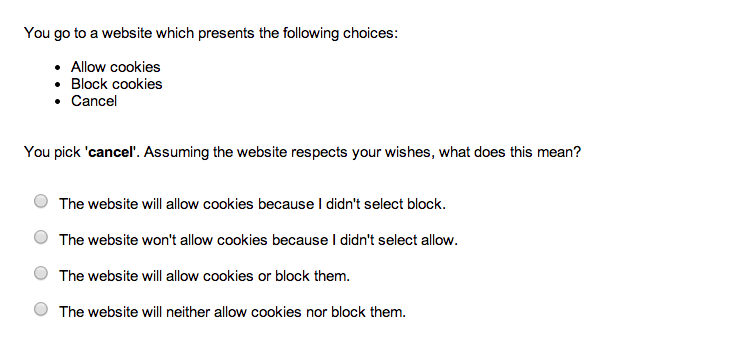
\includegraphics[scale=.5]{chapter5.tex/textcpcookie}
  }
\caption{Textual, Deontic Force, Cookie Condition}
\label{textcpcookie}
\end{figure}

\begin{figure}
\centerline{
  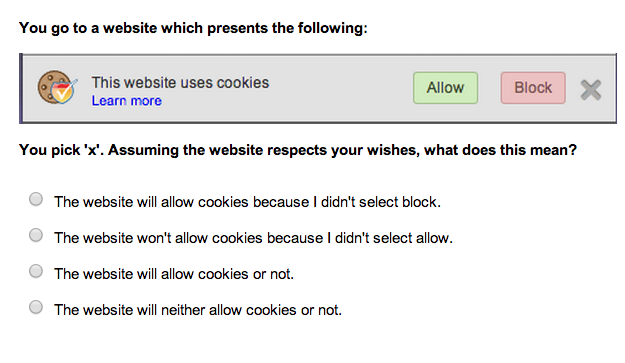
\includegraphics[scale=.5]{chapter5.tex/dialogcpcookie}
  }
\caption{Mixed-Modal, Deontic Force, Cookie Condition}
\label{dialogcpcookie}
\end{figure}


Answering either:

\begin{itemize}
\item The website will allow cookies because I didn't select block
\item The website won't allow cookies because I didn't select allow
\end{itemize}

was considered evidence of pragmatic implicature. 

\subsubsection{Instrumentation}
\label{instrumentation}


\begin{sloppier}
In addition to features provided by AMT and Qualtrics, my scripts performed the following:

\begin{enumerate}
\item Disable preview using a custom CSS class blocking Qualtrics controls
\item Check worker hash against a FireBase web service and request worker to return HIT if the hash is in the exclusion list
\item Add worker hash to FireBase
\item Submit results to AMT on completion of the Qualtrics survey
\end{enumerate}
\end{sloppier}


No other instrumentation was required for this experimental design.

\subsection{Experiment 1B Method}
\label{experiment1bmethod}

\subsubsection{Settings and Participants}
\label{settingsandparticipants}

Using Amazon's Mechanical Turk, 200 workers were paid \$0.15 to participate in one of two conditions of the single factor design previously described. Participants were assigned randomly via Qualtrics block randomizer. Results were collected between the days of 7--14 October 2013. The task was expected to take approximately three minutes, though workers were allowed up to 10 minutes to complete.

\subsubsection{Procedure and Materials}
\label{procedureandmaterials}

The general procedure follows that described in Chapter Four.  \autoref{1B-flow}  is a more detailed graphical depiction of flow.

\begin{figure}
\centerline{
  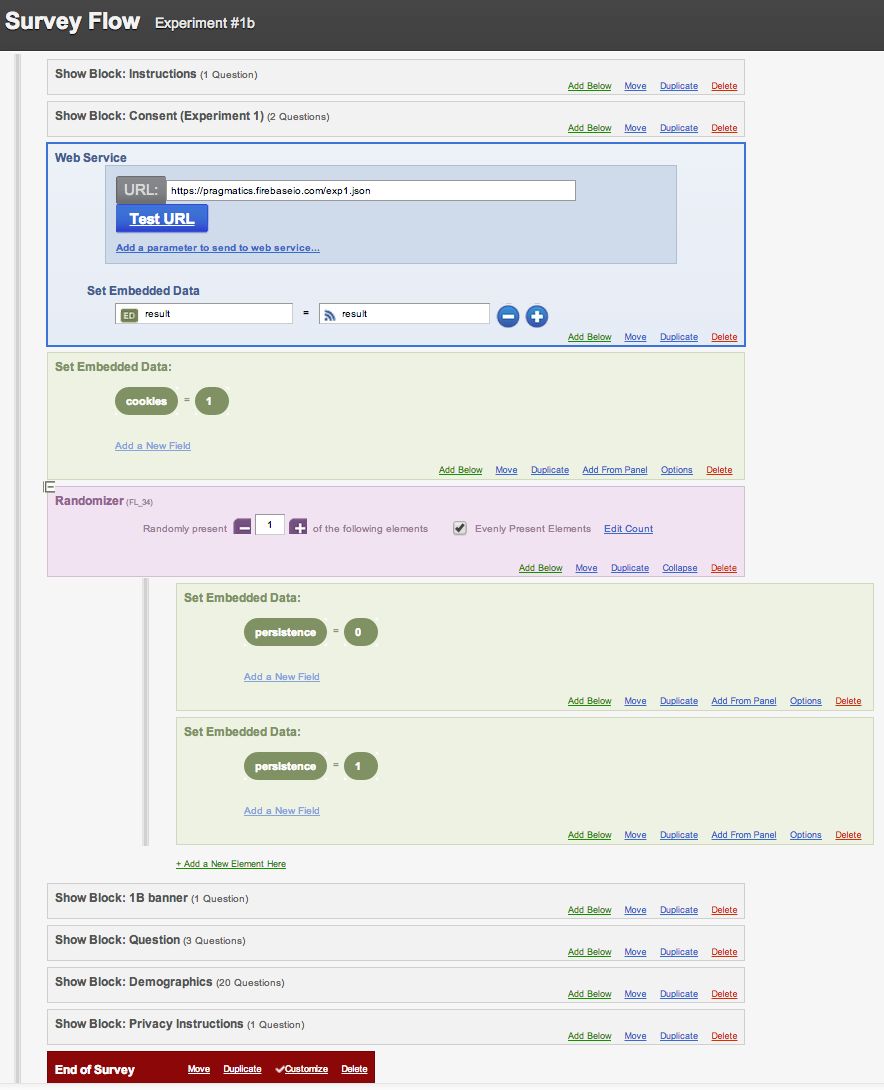
\includegraphics[scale=.4]{chapter5.tex/1b-flow}
  }
\caption{Experiment 1B Flow}
\label{1B-flow}
\end{figure}

Following presentation of instructions and consent form, participants were each presented a start screen with a cookie banner (appearance animated to draw attention), as illustrated in  \autoref{1B-start}. 

\begin{figure}
\centerline{
  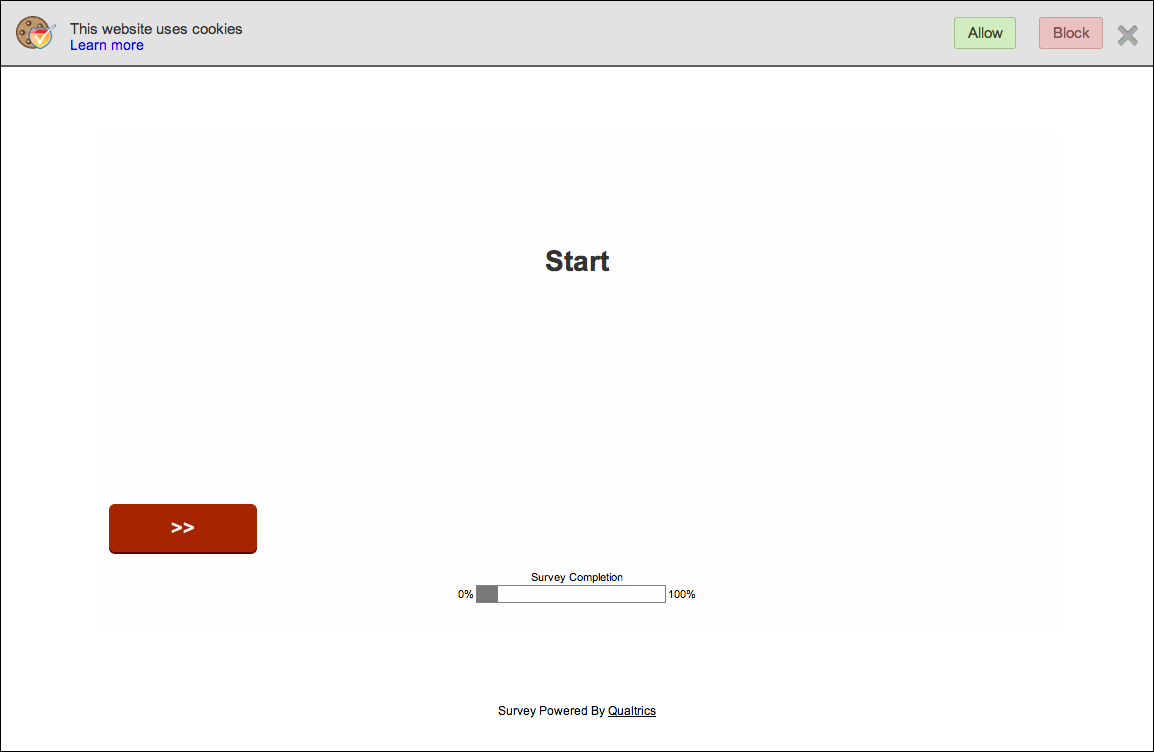
\includegraphics[scale=.3]{chapter5.tex/1b-start}
  }
\caption{Experiment 1B Stimulus}
\label{1B-start}
\end{figure}

Immediately following this, workers were presented with the following question:

\begin{quote}
Do you think there are ad trackers on this site?
\end{quote}


In the treatment condition ( \autoref{1B-feedback}),  participants were given feedback from their action on the previous screen.

\begin{figure}
\centerline{
  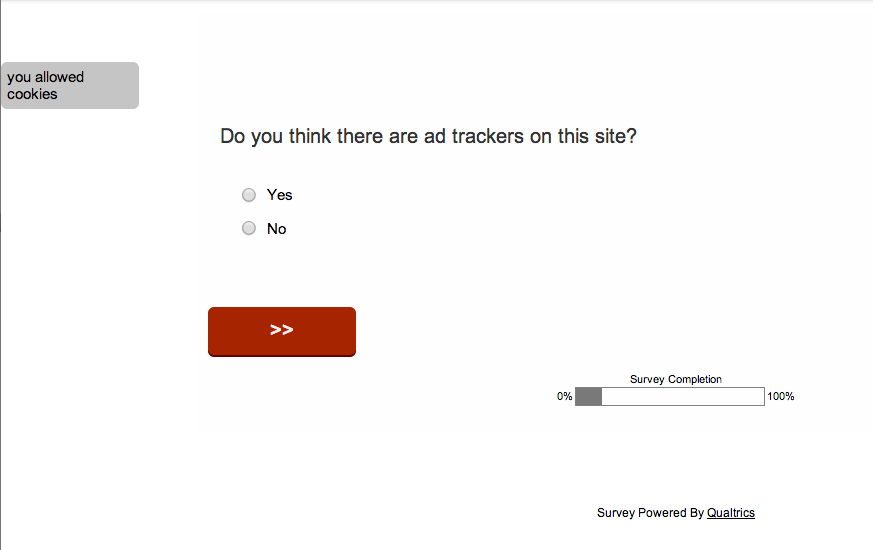
\includegraphics[scale=.4]{chapter5.tex/1b-feedback}
  }
\caption{Experiment 1B Question (with feedback)}
\label{1B-feedback}
\end{figure}

They were then asked if they believed there were ad trackers on the site  (\autoref{1B-belief}).  Finally, participants were asked about their beliefs on the basis of this response  (\autoref{1B-justification}). 

\begin{figure}
\centerline{
  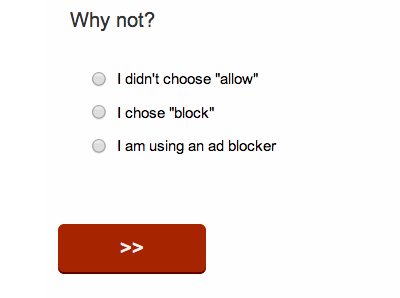
\includegraphics[scale=.5]{chapter5.tex/1b-no}
  }
\caption{Experiment 1B Cookie Belief}
\label{1B-belief}
\end{figure}


\begin{figure}
\centerline{
  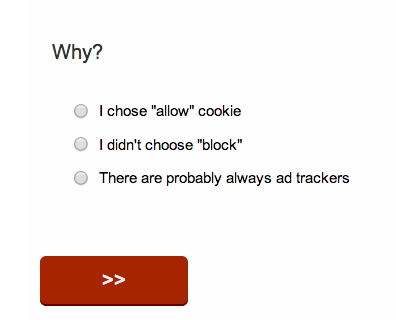
\includegraphics[scale=.5]{chapter5.tex/1b-yes}
  }
\caption{Experiment 1B Belief Justification}
\label{1B-justification}
\end{figure}


Responses were coded as implicature for the control group if the subject did nothing and responded with ``I chose allow'' \slash  ``I didn't choose allow'' (Yes) or ``I didn't choose block'' \slash  ``I chose block'' (No). In the treatment group ``I chose allow'' \slash  ``I didn't choose block'' (Yes) were not coded as implicature since feedback had been provided giving the subject knowledge of the consequences of their action.

\subsubsection{Instrumentation}
\label{instrumentation}

In addition to features provided by AMT and Qualtrics, my scripts performed the following:


\begin{sloppier}
\begin{enumerate}
\item Disable preview using a custom CSS class blocking Qualtrics controls
\item Check worker hash against a FireBase web service and request worker to return HIT if the hash is in the exclusion list
\item Add worker hash to FireBase
\item Submit results to AMT on completion of the Qualtrics survey
\item Display cookie banner on start page
\item Record button presses on the cookie banner (accept, block, learn more, close)
\item In the treatment condition, display feedback on the basis of cookie banner interaction
\end{enumerate}
\end{sloppier}


\section{Data Collected}
\label{datacollected}

Using G* Power 3 chi square goodness of fit test  \citep{PowerAnalysisIntro:2012uy},  for both experiments I estimated a sample size of approximately 220 was necessary in order to detect a medium effect with power of 0.95. All surveys initiated were completed: there were no known drop-outs.

Once all assignments had been completed, (as indicated on my AMT requester dashboard), I downloaded data as a single CSV (comma separated values) file from the Qualtrics website. Data was organized such that each participant's data was on its own row.

\section{Results}
\label{results}

In this section, I present experimental results for both experimental designs.

\subsection{Experiment 1A Results}
\label{experiment1aresults}

The two tables,  \autoref{text-conditions} and \autoref{mixed-modal-conditions}  , present raw percentages of implicature calculated for the three-factor design with 213 participants. Determination of implicature is dichotomous --- either the participant interprets an implicature or not. Thus, the top two answers for each question were rolled into a single dependent variable (implicature) for which a percentage value is displayed. Within  \autoref{text-conditions}  and  \autoref{mixed-modal-conditions}  are two contexts for interpretation: the participants believes that a cookie will be deposited in the browser or not.


\begin{table}
\caption{Implicature in Text Conditions}
\label{text-conditions}
\centering
\begin{tabular}{ccc}
 & \multicolumn{2}{c}{Text}\tabularnewline
\cline{2-3} 
Cookies & DF & 48\%\tabularnewline
 & No DF & 50\%\tabularnewline
\hline 
Pictures & DF & 67\%\tabularnewline
 & No DF & 50\%\tabularnewline
\end{tabular}
\end{table}



\begin{table}
\caption{Implicature in Mixed-Modal Conditions}
\label{mixed-modal-conditions}
\centering
\begin{tabular}{ccc}
 & \multicolumn{2}{c}{Mixed-Modal}\tabularnewline
\cline{2-3} 
Cookies & DF & 63\%\tabularnewline
 & No DF & 65\%\tabularnewline
\hline 
Pictures & DF & 72\%\tabularnewline
 & No DF & 67\%\tabularnewline
\end{tabular}
\end{table}


For analysis, a \textbf{basic difference statistics} is required. Because the IV is categorical (binary), a non-parametric statistics is required. A Pearson's chi-square test for independent samples is appropriate. However, its not possible to apply a chi-square test to tables with three or more discrete variables. In such a case, a \textbf{log linear model} is more useful. It has both the characteristics of a chi-square test determining the fit between observed and expected frequencies, as well as features of an ANOVA such that it is possible to do simultaneous testing of main effects and interactions within a fully factorial design.

For hypothesis 1A above, of primary interest are group differences associated with the main effect mixed-modal versus text. But we can also examine the 2-way interaction of privacy and 2-way interaction with deontic force in both textual and mixed-modal conditions.

\begin{sloppier}
In \autoref{loglinear}, independent and dependent variables are treated equally. It includes main effect plus 2-way and 3-way interactions. Where residuals are close to 0, the model has a better fit. I discarded the 4-way interaction (Graphics:DF:Privacy:Implicature) since it did not improve model fit. 
\end{sloppier}

\begin{table}
\caption{Log Linear Significance}
\centering
%% LyX 2.0.6 created this file.  For more info, see http://www.lyx.org/.
%% Do not edit unless you really know what you are doing.
%\documentclass[english]{article}
%\usepackage[T1]{fontenc}
%\usepackage[latin9]{inputenc}

%\makeatletter

%%%%%%%%%%%%%%%%%%%%%%%%%%%%%% LyX specific LaTeX commands.
%% Because html converters don't know tabularnewline
%\providecommand{\tabularnewline}{\\}

%\makeatother

%\usepackage{babel}
%\begin{document}
\begin{sideways}
\begin{tabular}{lcccccc}
\hline 
 & Df & Deviance & Resid. & Df Resid. & Dev & Pr(>Chi)\tabularnewline
\hline 
NULL &  &  & 15 & 28.6821 &  & \tabularnewline
Graphics & 1 & 0.0423 & 14 & 28.6398 & 0.8371346 & \tabularnewline
DF & 1 & 0.0423 & 13 & 28.5976 & 0.8371346 & \tabularnewline
Privacy & 1 & 0.0047 & 12 & 28.5929 & 0.9453725 & {*}{*}{*}\tabularnewline
Implicature & 1 & 13.3274 & 11 & 15.2655 & 0.0002616 & \tabularnewline
Graphics:DF & 1 & 0.1155 & 10 & 15.1501 & 0.7340215 & \tabularnewline
Grapics:Privacy & 1 & 0.0419 & 9 & 15.1082 & 0.8378711 & \tabularnewline
DF:Privacy & 1 & 0.2248 & 8 & 14.8834 & 0.6353792 & \tabularnewline
Graphics:Implicature & 1 & 7.3723 & 7 & 7.5110 & 0.0066235 & {*}{*}\tabularnewline
DF:Implicature & 1 & 0.0361 & 6 & 7.4750 & 0.8493662 & \tabularnewline
Privacy:Implicature & 1 & 0.0960 & 5 & 7.3790 & 0.7566902 & \tabularnewline
Graphics:DF:Privacy & 1 & 0.1101 & 4 & 7.2689 & 0.7400369 & \tabularnewline
Grapics:DF:Implicature & 1 & 1.8719  & 3 & 5.3970 & 0.1712625 & \tabularnewline
Graphics:Privacy:Implicature & 1 & 1.0591 & 2 & 4.3379 & 0.3034217 & \tabularnewline
DF:Privacy:Implicature & 1 & 4.2340  & 1 & 0.1039 & 0.0396209 & {*}\tabularnewline
\hline 
\multicolumn{7}{c}{Significance codes: 0 {*}{*}{*} 0.001{*}{*} 0.01{*} 0.05 0.1 1}\tabularnewline
\hline 
\end{tabular}
\end{sideways}
%\end{document}

\label{loglinear}
\end{table}


From the table above, \emph{there is a significant difference between text and mixed-modal conditions for implicature where p$<$.01: implicature is higher in conditions where users are presented mixed-modal information.} This validates my hypothesis that implicature may be communicated in mixed-modal conditions, just as it would in a purely textual context. What is, perhaps surprising, and interesting is that subjects are even more likely to interpret an implicature.

There is also a significant difference for implicature where deontic force occurs with pictures (p$<$.05). There is no firm basis for understanding why this may be the case. I speculate that this may be because subjects might ordinarily expect pictures to be displayed and thus might imagine that they were being asked if they wished to block them. For example, some email clients do not load pictures automatically, but explicitly ask users whether they would like to trust loading pictures for a particular sender.

Finally, there are some limitations to this analysis. For linguistic studies such as this, mixed model effects are often desired. A potential issue with my analysis is that it commits what  \citet{Clark:1973vn}  terms the ``language-as-fixed-effect'' fallacy. This means that the results do not generalize beyond the sample studied here. It is easy to understand how important this is in light that simply by changing the words ``accept'' \slash  ``block'' to ``on'' \slash  ``off'' we saw a tangible effect. This may well relate to the nature of deontic force implied by ``accept'' \slash  ``block'', but it could also be to other reasons. For example, it is possible that lexical and semantic features of other pairs such as ``yes'' \slash  ``no'' may may also affect findings.

Increasingly, language researchers are moving to mixed effects models which simply model fixed and random effects in a linear form. Random effects may be added for variables specific to the data sample such as effects relating to subjects, words, and other items. Such an analysis is not substantially more difficult than the one presented here. However, the log linear approach is adequate for the purpose of this pilot study.

\subsection{Experiment 1B Results}
\label{experiment1bresults}

 \autoref{1B-results}  below presents raw frequency counts for each of the two conditions (see also,  \autoref{1B-fig}). 


\begin{table}
\caption{1B Results}
\centering
%% LyX 2.0.6 created this file.  For more info, see http://www.lyx.org/.
%% Do not edit unless you really know what you are doing.
%\documentclass[english]{article}
%\usepackage[T1]{fontenc}
%\usepackage[latin9]{inputenc}

%\makeatletter

%%%%%%%%%%%%%%%%%%%%%%%%%%%%%% LyX specific LaTeX commands.
%% Because html converters don't know tabularnewline
%\providecommand{\tabularnewline}{\\}

%\makeatother

%\usepackage{babel}
%\begin{document}
\begin{tabular}{ccc}
 & Other & Implicature\tabularnewline
\hline 
Control & 79 & 22\tabularnewline
Feedback & 95 & 4\tabularnewline
\hline 
\end{tabular}
%\end{document}

\label{1B-results}
\end{table}

As before, because the IV is categorical (binary), a non-parametric statistics is required. Using a Pearson's chi-square test with a Yates' continuity correction, subjects in the feedback condition showed significantly less implicature than in the control condition,  $\chi^2$ (1,N=200)=12.39, p$<$.001. The odds of implicature are 6.6 times more likely when there is no feedback given.



\begin{figure}
\centerline{
  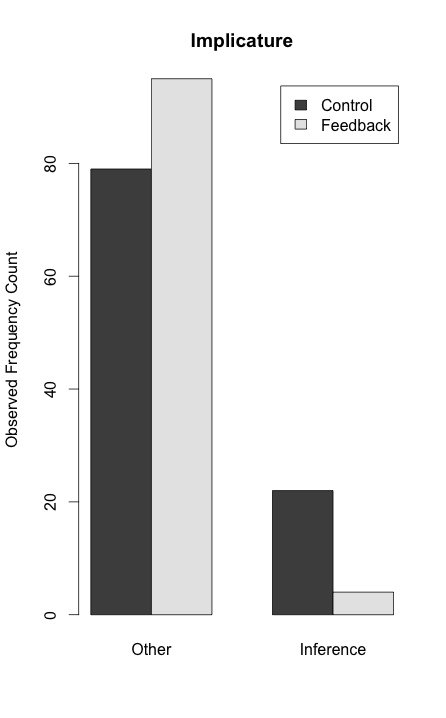
\includegraphics[scale=.5]{chapter5.tex/implicature}
  }
\caption{Implicature Per Condition}
\label{1B-fig}
\end{figure}


Of interest is that 30 participants in the control group and 33 in the treatment groups chose to ``accept'' cookies (and only 2 chose to ``block'';  \autoref{1B-clicks}). 


\begin{table}
\caption{Click Actions}
\centering
%% LyX 2.0.6 created this file.  For more info, see http://www.lyx.org/.
%% Do not edit unless you really know what you are doing.
%\documentclass[english]{article}
%\usepackage[T1]{fontenc}
%\usepackage[latin9]{inputenc}

%\makeatletter

%%%%%%%%%%%%%%%%%%%%%%%%%%%%%% LyX specific LaTeX commands.
%% Because html converters don't know tabularnewline
%\providecommand{\tabularnewline}{\\}

%\makeatother

%\usepackage{babel}
%\begin{document}
\begin{tabular}{ccccc}
 & Accept & Reject & Learn More & Dismiss\tabularnewline
\hline 
Control & 30 & 0 & 1 & 1\tabularnewline
Feedback & 33 & 2 &  & \tabularnewline
\hline 
\end{tabular}
%\end{document}

\label{1B-clicks}
\end{table}


Click results were different than observed in the pre-pilot. Possibly, some workers believed that that must accept cookies in order to participate. Or workers may have believed that the survey wouldn't work properly without accepting cookies. This indicates a potential bias for cooperation. This is also evidenced by one of the subject's comments:

\begin{quote}
I didn't figure, at first, that the thing about allowing cookies was part of the survey; I figured the survey was based in the UK and was trying to comply with the new UK laws about cookies. (I always allow cookies, because disallowing them creates more problems than allowing them does.)
\end{quote}
Several comments were along the lines of this one:
\begin{quote}
Wow, this definitely made me question whether I knew anything about cookies and ad tracking or not. The questions seemed super simple, but I realized I was making a lot of vague assumptions when you asked more specific questions.
\end{quote}

It is also useful to consider whether an implicature might result in harm. By harm, I mean whether the user infers there are no ad cookies. Non-harmful inference would occur in a situation where a participant believed there were ad cookies and also answered ``I chose allow'' or ``I didn't choose block'' yet took no action on the cookie banner --- inferring passive consent through inaction. On the other hand, an inference that is potentially harmful falls under the situation where the participant did not believe there were ad tracking cookies and responded, ``I didn't choose allow'' or ``I chose block'' yet took no action on the cookie banner --- inferring non-consent through inaction.

Under this interpretation of harm, approximately 10\% of those in the control group made harmful inferences while only 4\% in the treatment group. These 4\% made an incorrect inference ``I didn't choose allow'' despite very visible feedback to the contrary.

\chapter{Study Two: Hyperdeixis in Advertisements}
\label{studytwo:hyperdeixisinadvertisements}

How do we understand interaction with objects on the Internet? This study considers the role of reference in hyperlinked advertisements. Intentionally misleading or not, ``opt-out'' mechanisms for behavioral advertisements are not intuitive. I believe the cause for confusion is intimately aligned with how we process and understand linguistic signs.

\section{Motivation}
\label{motivation}

In 2009, under pressure from the FTC, industry advertisers formed an alliance called the Digital Advertising Alliance (DAA). The purpose was to establish self-regulatory principles for online behavioral advertising  \citep{AAAA:2009uc}.  These principles advocate transparency for:

\begin{sloppier}
\begin{quote}
[...] clearly disclosing and informing consumers about data collation and user practices with online behavioral advertising [...] Compliance with the Principle will result in new links and disclosures on the web page or advertisement where online behavioral advertising occurs. \citep[p. 2]{AAAA:2009uc}
\end{quote}
\end{sloppier}
Further: 
\begin{quote}
Links to consumer notices will be clear, prominent, and conveniently located... Such enhanced notice will be provided at the time of such collection and use, through common wording and a link/icon that consumers will come to recognize... One option for providing this... is for an entity to attach a uniform link/icon and wording to each advertisement that it serves. Click this link/icon will provide a disclosure from the entity in the form of an expanded text scroll, a disclosure window, or a separate page.  \citep[p. 5]{AAAA:2009uc}
\end{quote}
\begin{sloppier}
This section considers whether DAA self-regulation has designed an effective means for "enhanced notice". 
\end{sloppier}


\subsection{Advertiser Self-Regulation and AdChoices}
\label{advertiserself-regulationandadchoices}

DAA self-regulation has come under repeated fire. The implementation of enhanced notice is the AdChoices icon  (\autoref{adchoices}).  \citet*{Komanduri:2012wo}  examined DAA principles and came up with a list of ten requirements appropriate for compliance checks. Included was a check of whether participating advertisers complied with enhanced notice. One problem is that it is nearly impossible to tell whether a particular ad is behavioral or not. However, they report that according to industry estimates of the time, about 80\% of advertisements encountered are behavioral. Based on this statistic,  \citet{Komanduri:2012wo}  found serious compliance problem including infrequent compliance with ``enhanced notice''.


\begin{figure}
\centerline{

\includegraphics[scale=.5]{chapter6.tex/adchoices}
}
\caption{AdChoices Icon}
\label{adchoices}
\end{figure}


Separately,  \cite{J:2011wm}  manually inspected pages from 449 domestic websites from the Alexa list of top 500 U.S. websites for third-party ads. Only 11.3\% included an AdChoices icon in or around the ad.

Mayer also showed \autoref{original-adchoices} and \autoref{final-adchoices} on his blog at the Center for Internet and Society at Stanford Law School: \cite{J:2011wm}:

\begin{figure}
\centerline{
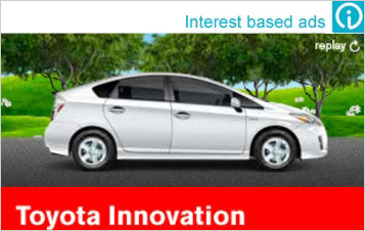
\includegraphics[scale=.75]{chapter6.tex/adchoices_original}
}
\caption{Original AdChoices Design}
\label{original-adchoices}
\end{figure}

\begin{figure}
\centerline{
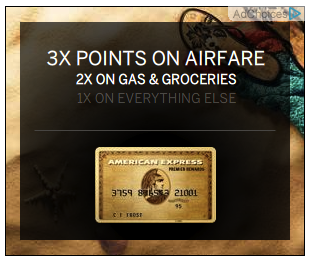
\includegraphics[scale=.5]{chapter6.tex/adchoices_icon_text}
}
\caption{Final AdChoices Design}
\label{final-adchoices}
\end{figure}


Note the differences. According to current DAA Creative Guidelines  \citep{Anonymous:2011ur},  icon only size with container is specified at 19x15 pixels with a rounded left corner radius and 70\% opacity. When embedded in an image, it should be in the upper right corner and there should be no space between it and the ad corner.

\subsection{Effectiveness of the AdChoices Icon}
\label{effectivenessoftheadchoicesicon}

In October of 2012, Evidon served about two billion AdChoices privacy notices daily  \citep{Otlacan:0FDP0X6N}.  This includes delivery across 40 countries and 38 languages. Earlier in 2011, Evidon reported 500,000 ``opt-outs'' as a result of presenting over 50 billion ads  \citep{Dunaway:dVJ7JFhh}.  However,\\

\begin{quote}
[...] those are not "user opt outs" but "company opt outs." For example, if a browser hits an advertiser's opt-out page on Evidon that has 10 ad tech companies listed total, if all are opted out, that counts as 10 opt-outs, even though it's just one browser. \citep{Dunaway:dVJ7JFhh}
\end{quote} 

Disregarding this,  \citet{Dunaway:dVJ7JFhh}  reports the rate of ``opt-out'' at 0.0046\% and  \citet{Logic:2011wn}  reports 0.0035\%.

 \citet{AdChoicesOurExpe:2012ux}  further reports from the period of January 2012 to mid-May 2012, the average daily activity of icon activity was 0.009\% (clicks\slash impression). Of these, 0.003\% were users who had set ``opt-out'' cookies in their browsers.

 \citet{Logic:2011wn}  notes that ``engagement'' in opt-out campaign is influenced by the prominence of the icon --- a white icon container on a black ad --- results in the highest click rates. They also note that ``transparency doesn't foster opt-out''. 1 in 700,000 people who see the icon actually opt-out (about 0.0001\%). Furthermore, they calculate that about 1 in 5 people who make it to the opt-out page actually opt-out. 

It's important to note that that, though AdChoices was introduced in 2010, its rollout to comply with European law was compliancy by 30 June, 2012  \citep{Anonymous:iPLCQu77}. 

\subsection{AdChoices and Confusion}
\label{adchoicesandconfusion}

In a study conducted by  \citet{Ur:2012ws},  48 participants were asked about their familiarity with the DAA advertising icon and older ``Power I'' icon. First, they were presented enlarged icons and tag lines with context. 41 responded they had never seen the icons. Later, presented in context next to advertisements, 25 participants still stated then had never before seen the icons while 8 more were unsure. Only 5 participants thought the icon was intended to provide information about OBA.

This report highlights many usability issues surrounding OBA, to include notice and choice mechanisms. However, they did not address the cause of why AdChoices appears so ineffective.

\subsection{What Makes a Good Ad Design?}
\label{whatmakesagoodaddesign}


\begin{sloppier}
While there is controversy about the effectiveness of "enhanced notice", the advertising industry is actually very good at design. In an online Banner Ad Design Web clinic \citep{BannerAdDesign:2011tg}, Flint McGlaughlin describes three key objectives that banner ads must accomplish in order to drive "maximum conversion".
\end{sloppier}
\begin{enumerate}
\item \textbf{Attract interest.} McGlaughlin gives examples from A/B market tests manipulating size, shape, color, motion, and position toward ad effectiveness.
\item \textbf{Generate interest.} In this, Mclaughlin and others (for example, posts concerning banner ad effectiveness on \url{http://retargeter.com}) focus on the need to understand where targeted consumers might be in the buying process. This principle speaks primarily to tailoring the message to an intended audience.
\item \textbf{"Ask for the Click."} Finally, McLaughlin emphasizes the need for a "call for action". While Internet users implicitly understand that ads are representative of the target site to which they are linked, by placing the image of a button in an ad, McGlaughlin stresses that clarity of the message is increased.
\end{enumerate}


In  \autoref{askforclick} from \cite{BannerAdDesign:2011tg}  and associated audio transcript below, \emph{it is clear to see that while advertisers believe that, despite an understanding that ads convey an implicit message to click, conveying this explicitly is vital}.


\begin{figure}
\centerline{
  
\includegraphics[scale=.25]{chapter6.tex/banner}
  }
\caption{Example "Ask for the Click" \citep{BannerAdDesign:2011tg}}
\label{askforclick}
\end{figure}
\begin{quotation}
Not this, here is an ad [left]. It is animated. They have got motion. Never mind the ugly color. Never mind that it screams the entire time you are looking. Never mind that you have to watch it for a long time before you get the message. Just consider the fact that even once you have watched the whole message, you don't know what to do.

To this, now this ad on the right shows...clearly, we could optimize this way better, but let's just look at this to learn from it. I see a picture of what I am getting, and because it is in a set of hands, I can actually get a sense of the size, and I can imagine it. Never promise a download or any other incentive that you don't help the audience visualize or imagine. Secondly, in the cover and in the key content of the cover, there is appeal already built for somebody in this space, and it is a well-known brand, and then, here it says, get everything you need to know about antiques right in the palm of your hand.

That is also quite helpful in understanding what the offer is, but these people have identified that at this stage, the person may not be ready to buy the book. They may want more info. That is the difference between saying a button 'Buy It Now'. You know, 'Get Your Copy' and instead 'Learn More'. \citep{BannerAdDesign:2011tg}
\end{quotation}


Finally, by regarding current ad images on  \url{http://moat.com} (\autoref{moat}),  it is evident that iconic buttons in image-based ads are highly desirable. This is the case, whether these are flash-based ads (buttons are functional) or simple image-based ads (buttons merely iconic).


\begin{figure}
\centerline{
  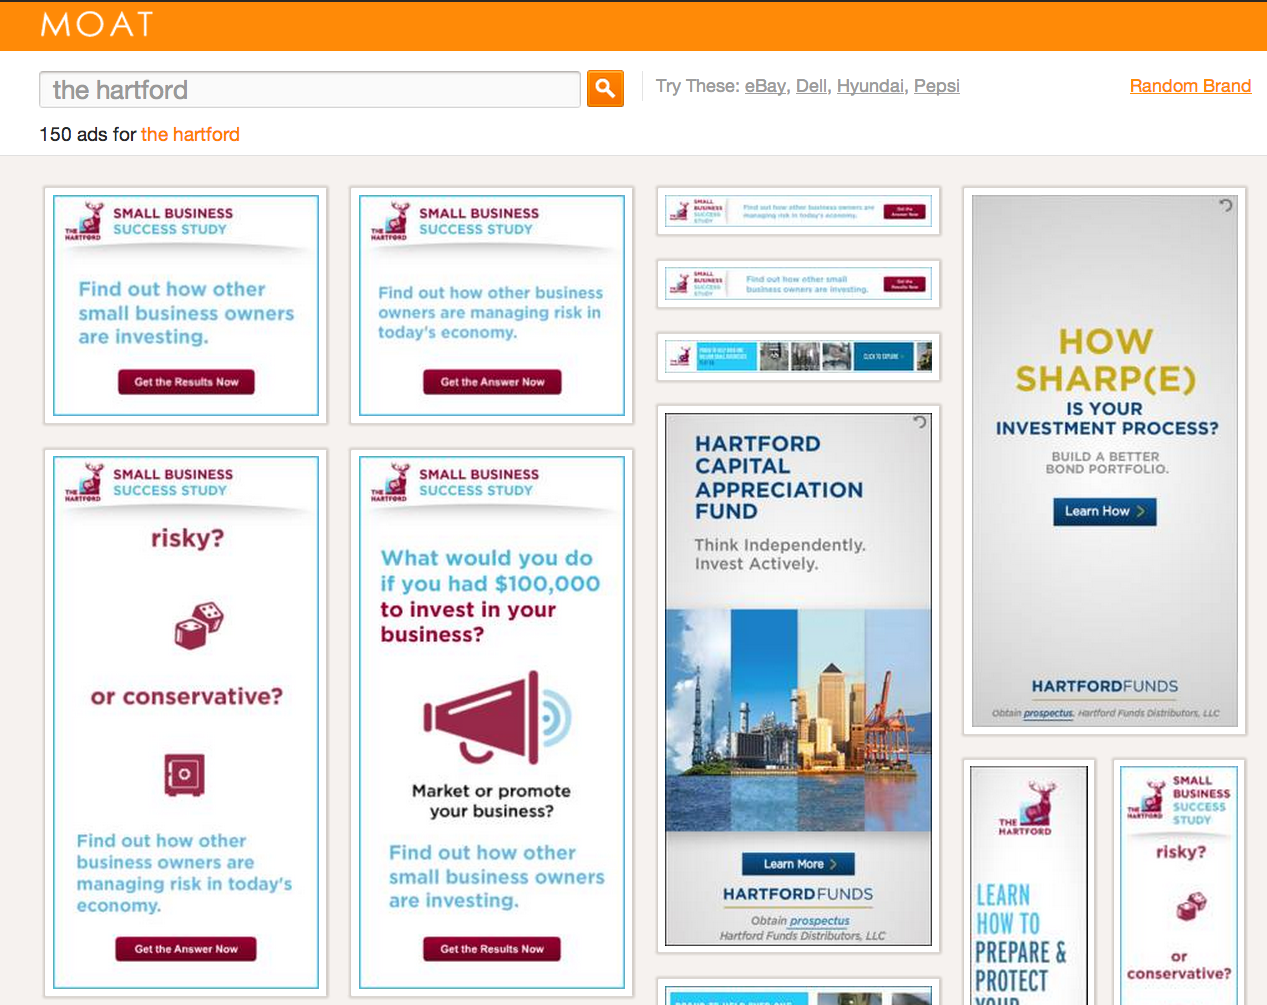
\includegraphics[scale=.25]{chapter6.tex/moat}
  }
\caption{Screen Capture from \url{http://moat.com}}
\label{moat}
\end{figure}


\section{Related Research}
\label{relatedresearch}

Advertising is an intensely competitive business, so it is not surprising that specific details about the effectiveness of the AdChoices icon are difficult to ascertain. Research presented below is directed toward iconicity and indexicality of ads and their parts. This relates to the notion of a ``call-to-action''.

\subsection{Salience}
\label{salience}

Foundational to the representational use of an icon in an ad is whether or not it is perceived in a composite image. Low-level visual properties have a potentially large effect on users.  \citet*{Hoffman:1997vx}  find that the saliency of a part depends on at least three factors: size relative to the whole object, degree to which it protrudes, and strength of its boundaries. They find that these factors influence visual processes determining the choice of figure and ground.  \citet*{Elazary:2008jk}  furthermore find that the selection of interesting objects in a scene is also largely constrained by low-level visual properties. In 76\% of images studied, one or more of the top three salient locations fell on an outlined object. 

By contrast, top-down models of attention concern the effects of objects and semantic relevance. In studies of task salience,  \citet*{Hegarty:2010ex}  find that good display design facilitates performance by highlighting visual features representing task-relevant information.

While visual saliency is concerned with how well an object stands out from other objects, cognitive saliency is concerned with the relative importance of information.  \citet{Schmid:2007vq}  describes cognitive salience as concepts directly activated and loaded into current working memory or via spreading activation where one concept activates another (e.g., ``dog'' activates ``bark'', ``fur'', ``poodle'', etc.). But he also makes reference to ontological saliency, described as a more stable property of objects. He gives the example of a photograph where dog is more salient than the field in the background. Cognitive saliency seems to refer, in part to the effect of visual properties in foregrounding and backgrounding, but also of the ontological saliency of objects, in general.

\begin{sloppier}
Cognitive salience is important to understanding the referential use of language in production and comprehension. \citet{Gundel:1993uq,Gundel:2012kq} account for the lexical expression of referring forms via two kinds of information: conceptual information about a speaker's intended referent, and procedural information about the assumed cognitive status of that referent in the mind of the addressee. That is, the more accessible an entity is to an addressee, the less information a referring expression needs to contain to be correctly understood. 
\end{sloppier}
So, for example, imagine the scene where two people are in a room where there is a basket of apples on a table. Person A notices person B looking at the apples and says, 
\\
\\
"Are you hungry? Please take \underline{one}."
\\
\\
The apples are present and, in fact, are uniquely identifiable. If they had not been, Person A might have said, 
\\
\\
"Are you hungry? Would you like an apple?"
\\
\\
The apples were highly salient so a pronominal form of reference contained enough information for Person B to understand the referent. With respect to visual scenes, \citet*{Vogels:2011wj} note that visually salient referents are more activated in memory and are thus better accessible than less visually salient referents. In controlled experimentation, expressions referring to visually salient entities tended to be more reduced. 


\subsection{Deixis}
\label{deixis}

Deixis is a type of linguistic reference that depends on context for understanding. For example, context can be linguistic as in:

\begin{enumerate}
\item Julie went to the library. \underline{She} was there all day.

The pronoun anaphorically points to a referent in previous linguistic context. Deictic reference can also be extra-linguistic.

\item I'll take \underline{that} one (\underline{pointing} to item in a glass case).
\end{enumerate}
\citep{SantaCruzlectures:1971te} distinguishes between several sorts of deixis which he identifies as \textbf{gestural}, \textbf{symbolic}, and \textbf{anaphoric}. A gestural use of a deictic expression is like sentence (2) above where a demonstrative is accompanied by a pointing gestures. It relies on the hearer monitoring some aspect of the physical situation.
 
Sentence (3) below exemplifies a symbolic deictic expression.
\begin{enumerate}[resume]
\item \underline{This} administration doesn't know what its doing.
\end{enumerate}

It's interpretation depends on a hearer knowing about some aspect of the communicative situation. Finally, an anaphoric use of an expression is one which can be interpreted by knowing what other part of discourse expression is coreferential with it. Sentence (1) above exemplifies this.

Deictic reference is particularly problematic in pragmatic understanding because it involves subjective, attentional, intentional, and other context dependent properties  \citep{Levinson:1983ww}. 

\begin{quote}
The difference between deictic \& non-deictic conceptions can be understood by analogy. Consider the difference between a sculptured representation of a human figure, set up in the middle of a courtyard, and a photograph of a human figure. The sculpture does not represent any particular observer's-point-of-view, but the photograph does. The photograph does because the camera had to repositioned at a particular place in front of or to the side of, above or below, or on the same level as, the model." \citep[p. 235]{SantaCruzlectures:1971te}
\end{quote}


\subsection{Indexicality and Knowledge}
\label{indexicalityandknowledge}

Semiotician Charles Peirce influenced theories of reference through his work on signs. In Peirce's semiotic theory there are three basic types of signs: \emph{icons}, \emph{symbols}, and \emph{indexes}. Every sign stands for something --- some object. What distinguishes them is the relation between the sign and the object. Icons resemble their object and, therefore, depend on perceptual knowledge. Symbols depend on communicative associations between sign and object. And indexes are ``physically connected'' --- they depend on knowledge about the connection in order to relate index to its object. Indices simply direct attention-to and refer to objects but, otherwise, assert nothing  \citep{Atkin:2005wd,Clark:2003tn}.  However, pre-requisite for understanding the referent of an index is \emph{knowing the relation between the index and its object}.

\subsection{Demonstrative Reference}
\label{demonstrativereference}

In study of demonstrative reference,  \citet{Kaplan:1980te}  characterized demonstration as directing intention, where the demonstration itself does not determine the referent. What he meant is that the demonstration is simply an ``externalization'' of intent  \citet[p. 589]{Kaplan:1980te}.  The demonstratum --- pointing --- has no intrinsic meaning: recognizing speaker intent is key.

In the case of a hypertext link, visual cues (e.g., color of digital ink, mouse hand icon) indicate the presence of a link. This link is indexical to some other body of text. After brief introduction, users understand that this relationship as indexical. But even when visual cues are not available, users may still infer an indexical relation.

In order for deixis to be effective, speakers communicate using signals with the intention to produce awareness. In this rests a coordination problem.  \citet{lewis69}  describes two ways in which indexicals may be established through convention: precedence and salience. He gives the example where he comes upon a patch of quicksand and wants to warn others of its presence. He puts up a scarecrow up to its chest hoping that whoever sees it will understand. He intends to produce awareness, but there is no established convention for communicating quicksand. This he hopes is communicated through force of salience. And through precedence. And at some point in time, as a signal becomes more salient, its indexicality is established through convention.

\subsection{Hyperdeixis}
\label{hyperdeixis}

How do Internet users know advertisements are indexical? Often, there are perceptual cues. Mouse rollovers change the iconic representation of a mouse cursor to a pointer. Often visual cues are available, such as text color. More important, advertisements are known to be indexical through convention. 

But what about complex images or graphics where the user can perceive no discernible change in the cursor nor other physical attributes to cue off? For example, would you expect the  \autoref{complex-image}  to be indexical, or the parts themselves to be indexical?


\begin{figure}
\centerline{
 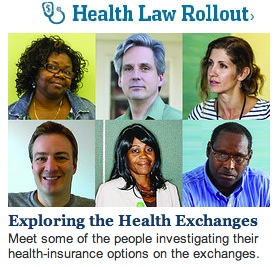
\includegraphics[scale=.5]{chapter6.tex/multipart-image}
}
\caption{Complex Image}
\label{complex-image}
\end{figure}


In the pre-pilot described in the next section, users did not agree on indexicality. Some thought the image linked to one unique location, and others thought each part of the image linked to a unique location. (In fact, the latter were correct, but the group was divided evenly.)

In light of the discussion above, features of advertising images I am most interested in examining are:

\begin{enumerate}
\item \textbf{Indexicality} - By convention, users know that to click on an image-based advertisement is to direct them to the advertiser's website. 
\item \textbf{Iconicity} - Buttons iconically communicate that an action may be performed and, depending on the context, have an indexical relation with a target webpage.
\item \textbf{Brand symbols} - Brands are indicative of particular companies and may also be indexical in an online context.
\end{enumerate}

A single advertisement can contain all of these attributes in combination. Some advertisements can become quite complex to the point of containing multiple microinteractions.


\begin{figure}
\centerline{
  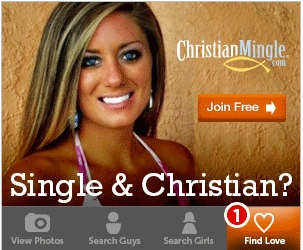
\includegraphics{chapter6.tex/complex}
  }
\caption{Complex Advertisement}
\label{complex-ad}
\end{figure}


As in the case of the complex image in  \autoref{complex-ad},  visual and perceptual cues (e.g., mouse cursor change to iconic hand) may not help users identify either indexicals or referents.

While  \citet{Loehr:1997uq}  refers to hypertext deixis as anchored links between text on a webpage to some other text, I refer more generally to such links as examples of \emph{hyperdeixis}. Arguably, user interaction online has become sophisticated to the point where one could dream up any sort of interaction and make it happen. For example, there is no intrinsic reason that hyperlinked text couldn't point to multiple objects. It would not be difficult to create this effect using simple JavaScript: a user mouses over text and a multi-option select box pops into view.

However, there is ample corpus-based linguistic evidence to suggest that we conceive of hyperlinks as ``pointers''. When we talk about hyperlinks, we use spatial metaphors. In  \autoref{ngram-plural} and  \autoref{ngram-singular},  it's easy to plot the use and distribution of the word ``hyperlink'' by its usage in modern media. Hyperlinks go ``to'' and ``from'' locations and are things ``between'' objects. They are also found ``in'' or ``on'' web text.


\begin{figure}
\centerline{
  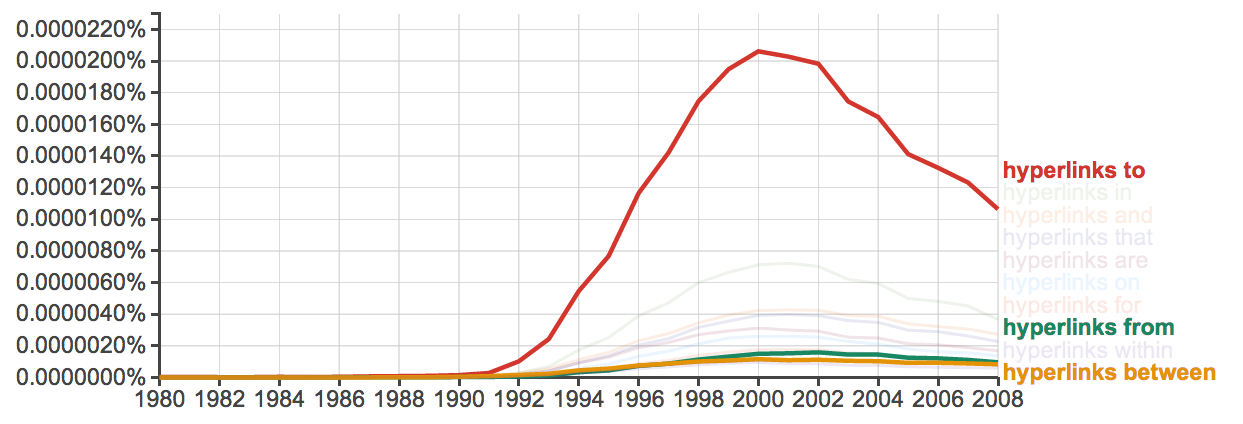
\includegraphics[scale=.25]{chapter6.tex/ngram1}
  }
\caption{Google Ngram Viewer (hyperlinks *)}
\label{ngram-plural}
\end{figure}



\begin{figure}
\centerline{
  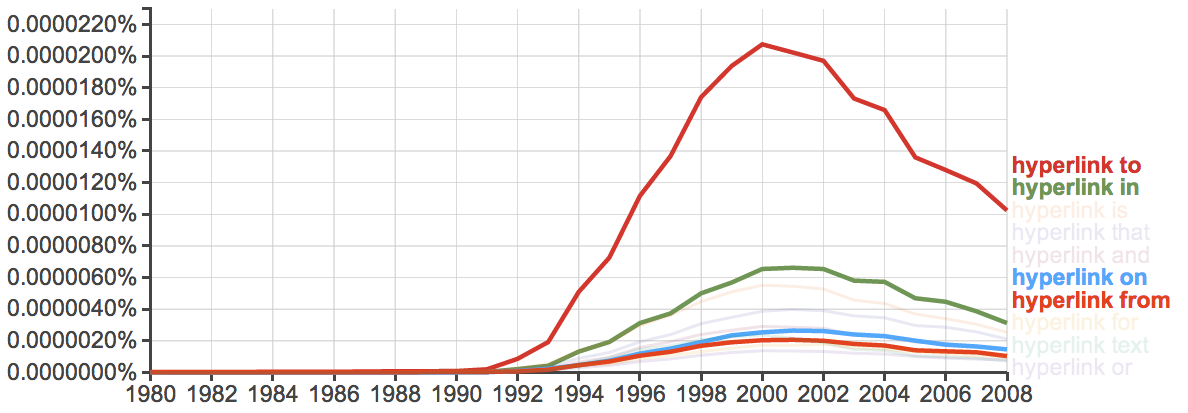
\includegraphics[scale=.25]{chapter6.tex/ngram2}
  }
\caption{Google Ngram Viewer (hyperlink *)}
\label{ngram-singular}
\end{figure}
\begin{sloppier}
In some sense, we are wired to understand the world this way.  Our conceptual system has properties grounded in perception --- both physically and socially \citep{Lakoff:2008tq}. Thought and reason are not simply linguistic abstractions but come from an intimate understanding the physical world around us.
\end{sloppier}


\subsection{Usability of Hyperlinked Icons}
\label{usabilityofhyperlinkedicons}

There appears to be little relevant research (if any) on the topic of hyperlinked images. However, there exists some on the topic of icons.  \citet*{Cheng:2007eh}  studied the use of iconic hyperlinks on e-commerce websites. Not surprisingly, they found that easily identifiable icons increase system usability. Those that are ambiguous affect the rate of task performance.  \citet*{Wiedenbeck:1999vk}  specifically examined the effect of combining text labels with icons. For a learning-based task, performance was poorest on icon-only interfaces, however, once learned, perception of ease of use was higher.

The pre-pilot discussed in the next section explores how people understand indexicality in the context of advertisements.

\section{Pre-Pilot}
\label{pre-pilot}

The purpose of this pre-pilot was to better understand how users perceive and interact with advertisements composed of graphical and iconic elements. 

\subsection{Method and Procedure}
\label{methodandprocedure}

Between the dates of 7--14 October 2013, I created an AMT assignment for 10 workers to annotate a series of approximately 25 images. For this task, I paid \$0.75. 

There were two groups of images representing two tasks. The first four image annotations were a test to see whether there might be a tangible effect of a ``call-to-action'' button icon on an ad. That is, would the presence of an iconic button influence where a person clicked on an ad. For these images, participants were given a screen shot of a digital news article and asked ``Please find the [Ford] Ad and click on it'' (substituting the brand name as appropriate).

The 21 remaining images comprised the second task which explored participant perception of image advertisements, including those containing the AdChoices icon. Workers were presented ads in isolation and asked to click on ``clickable things''. 

Before the second set of images was presented, I provided a short training session to familiarize annotators with the task. 

For the first training task  (\autoref{training-1}),  annotators were asked simply to click on the ad. By clicking, a tiny sticky note was left behind to remind the annotator where they clicked. Annotators were also asked to count the number of clickable things (things that do something or take you somewhere). For the first image, annotators were instructed to select ``1''.


\begin{figure}
\centerline{
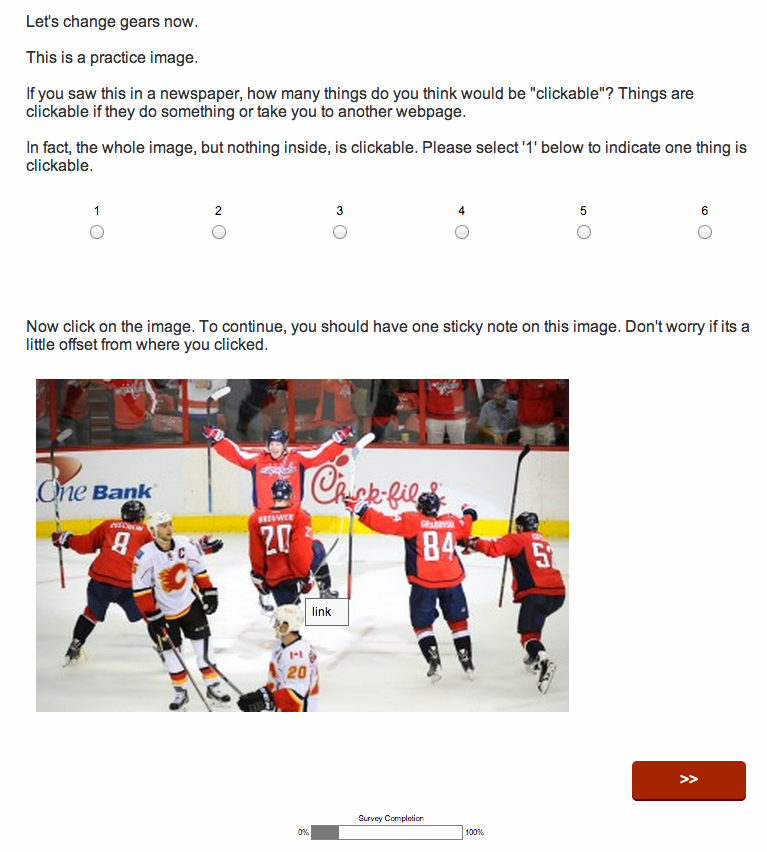
\includegraphics[scale=.3]{chapter6.tex/training1}
}
\caption{Training Task 1}
\label{training-1}
\end{figure}


For the second training task, a typical sign-in \slash  registration box was presented. Participants were instructed that text links and buttons from forms were clickable, but that text entry fields were not  (\autoref{training-2}). 


\begin{figure}
\centerline{
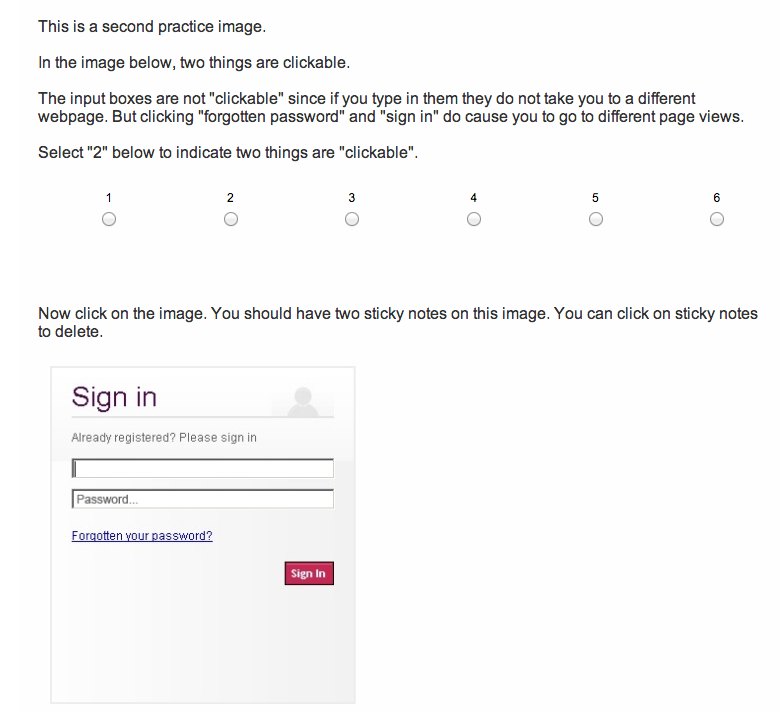
\includegraphics[scale=.3]{chapter6.tex/training2}
}
\caption{Training Task 2}
\label{training-2}
\end{figure}


Finally, in the third training task, participants were told that there were multiple things one could click on, but there were only three links  (\autoref{training-3}). 

\begin{figure}
\centerline{
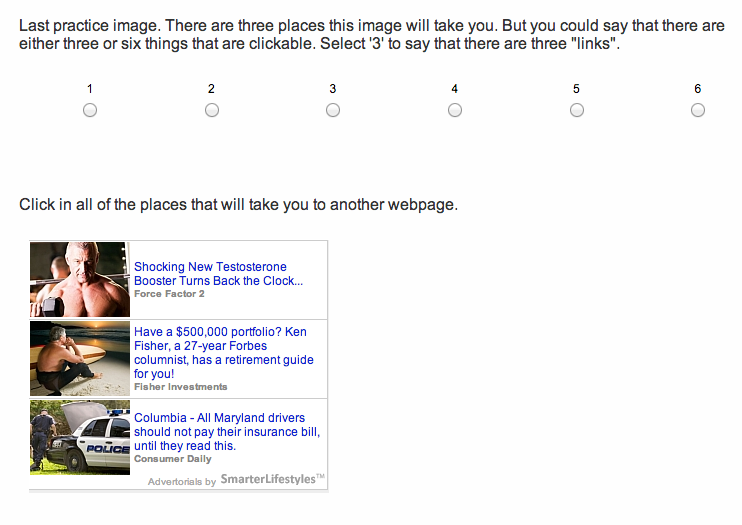
\includegraphics[scale=.3]{chapter6.tex/training3}
}
\caption{Training Task 3}
\label{training-3}
\end{figure}


After annotators completed all three training tasks, they were presented images to annotate on their own. A typical image annotation task is shown in  \autoref{prepilot-task}. 


\begin{figure}
\centerline{
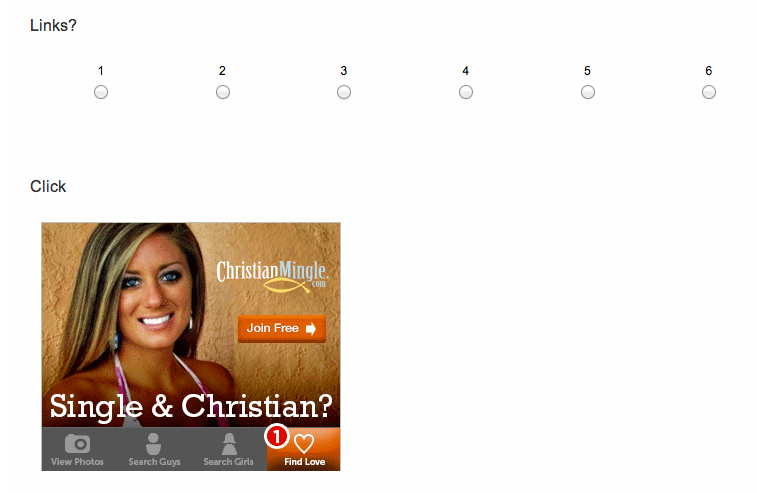
\includegraphics[scale=.3]{chapter6.tex/example1}
}
\caption{Image Annotation Task}
\label{prepilot-task}
\end{figure}


\subsection{Results and Discussion}
\label{resultsanddiscussion}

Results from the first four heat map visualizations appear in  \autoref{prepilot-ford}, \autoref{prepilot-cars}, \autoref{prepilot-travelers}, \autoref{prepilot-visa}. 


\begin{figure}
\centerline{
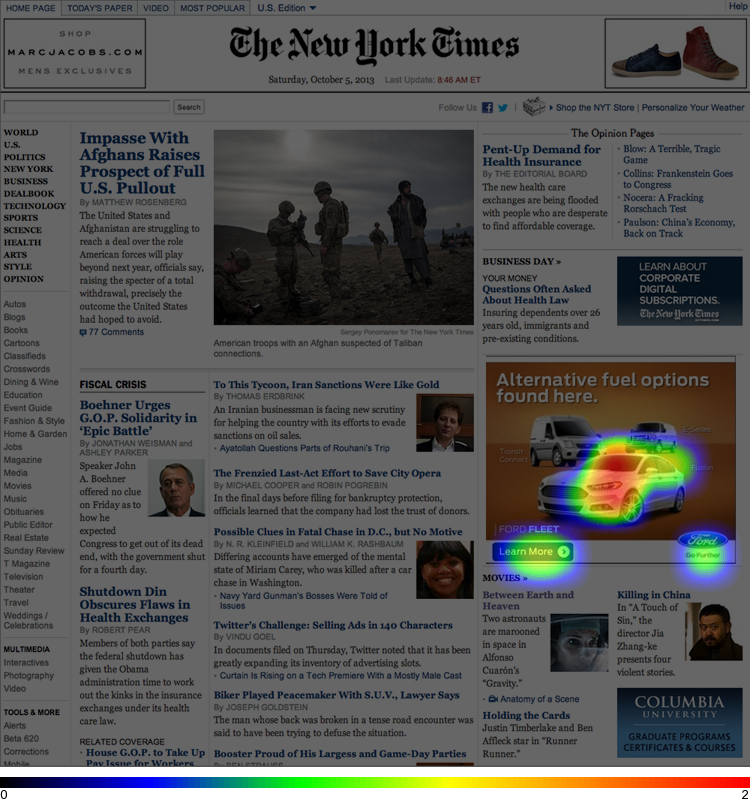
\includegraphics[scale=.3]{chapter6.tex/ford-hotspot}
}
\caption{Ford Ad}
\label{prepilot-ford}
\end{figure}

\begin{figure}
\centerline{
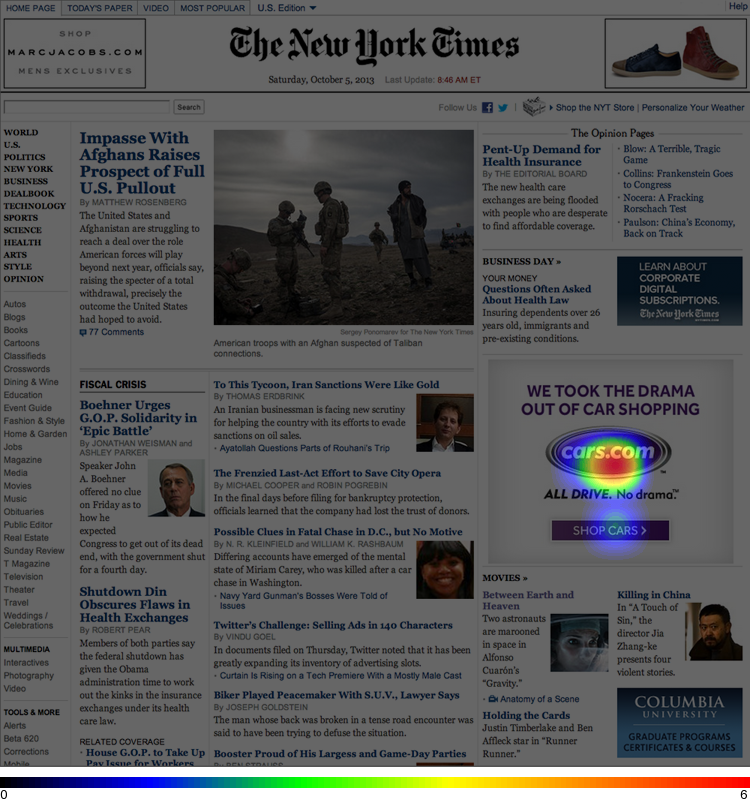
\includegraphics[scale=.3]{chapter6.tex/cars-hotspot}
}
\caption{Cars.com Ad}
\label{prepilot-cars}
\end{figure}

\begin{figure}
\centerline{
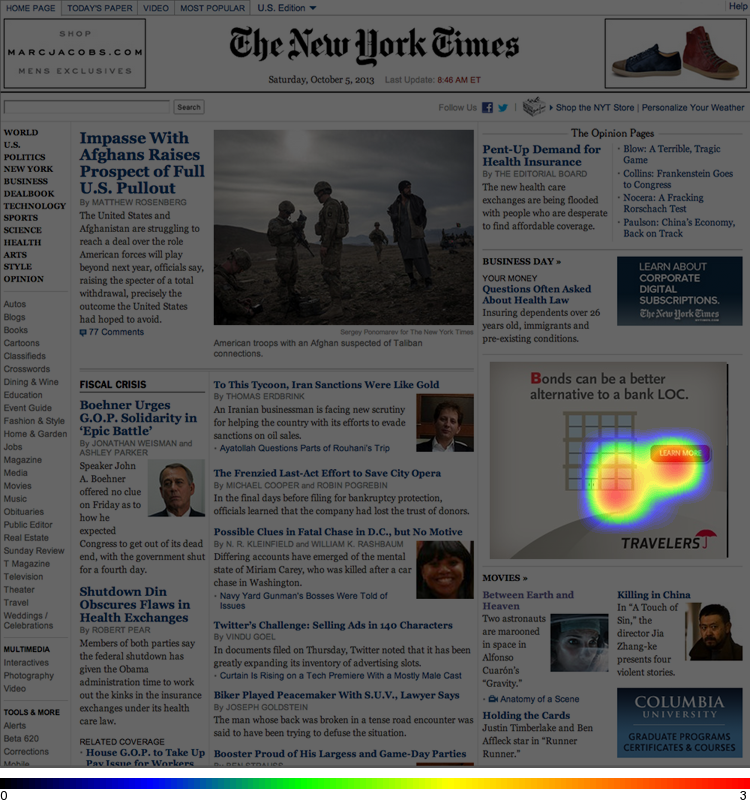
\includegraphics[scale=.3]{chapter6.tex/travelers-hotspot}
}
\caption{Traveler's Ad}
\label{prepilot-travelers}
\end{figure}

\begin{figure}
\centerline{
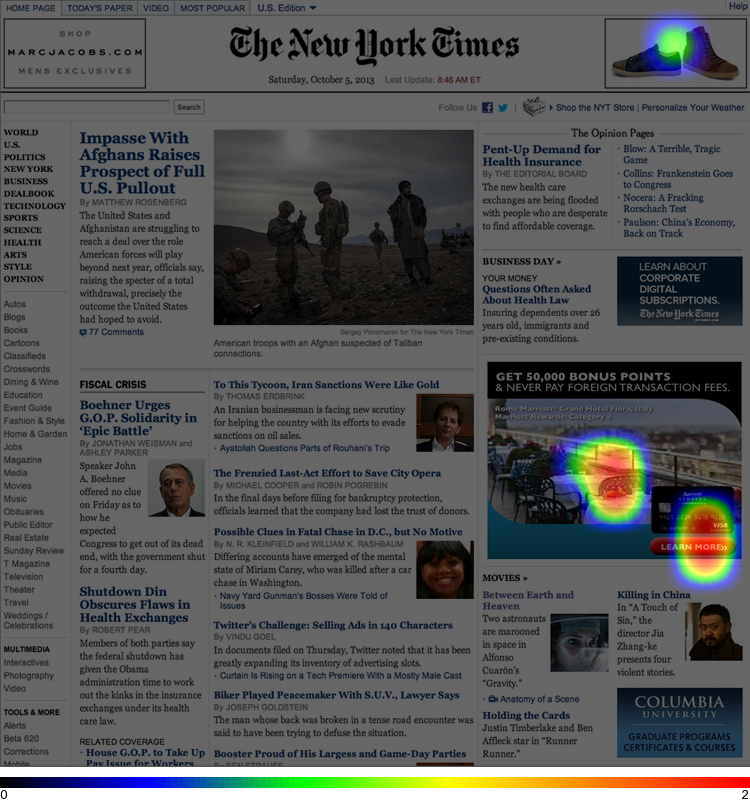
\includegraphics[scale=.3]{chapter6.tex/visa-hotspot}
}
\caption{Visa Ad}
\label{prepilot-visa}
\end{figure}

In each of the four images, one or more participants clicked directly on the iconic button link, despite implicit knowledge that the ad itself was hyperlinked to the advertiser's landing page. In addition, it appears that brands iconic in shape and style as buttons, also elicited clicks. Note the distinctive shape of the Ford logo in the first image and cars.com logo in the second. However, it could also be said that most clicked on the center of an ad, rather than on a button or iconic brand image.

 \autoref{complex-result}  shows the result for the example task 2 image above:

\begin{figure}
\centerline{
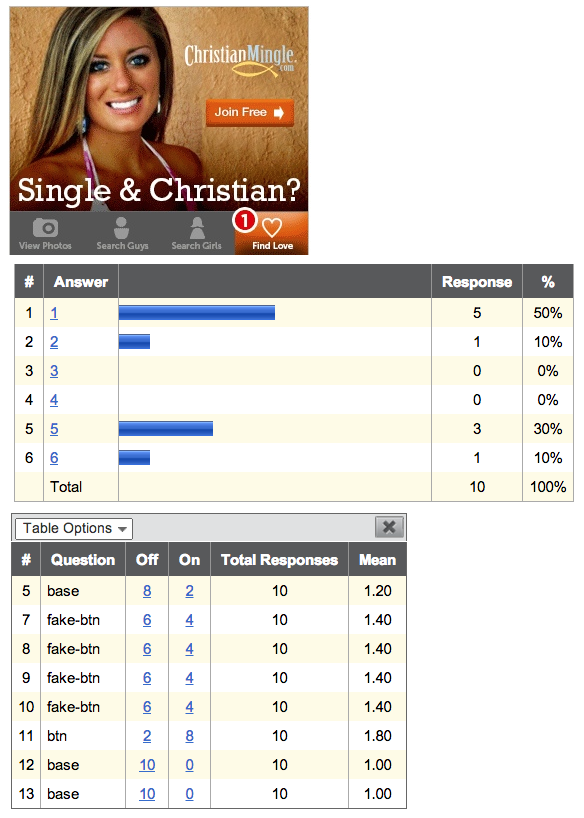
\includegraphics[scale=.3]{chapter6.tex/example1-annotated}
}
\caption{Results for Complex Ad}
\label{complex-result}
\end{figure}

Roughly half of the participants saw this ad as containing only one link. Others appeared to see fake buttons as links.

 \autoref{prepilot-twitter}  is another example from task 2. Here you can see that half of the annotators clicked on the Twitter icon.

\begin{figure}
\centerline{
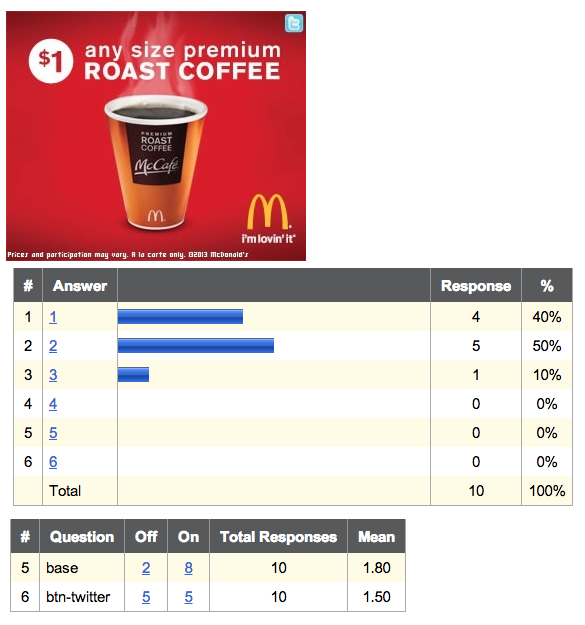
\includegraphics[scale=.5]{chapter6.tex/twitter-example}
}
\caption{Results for McDonald's Ad with Twitter Icon}
\label{prepilot-twitter}
\end{figure}



\begin{figure}
\centerline{
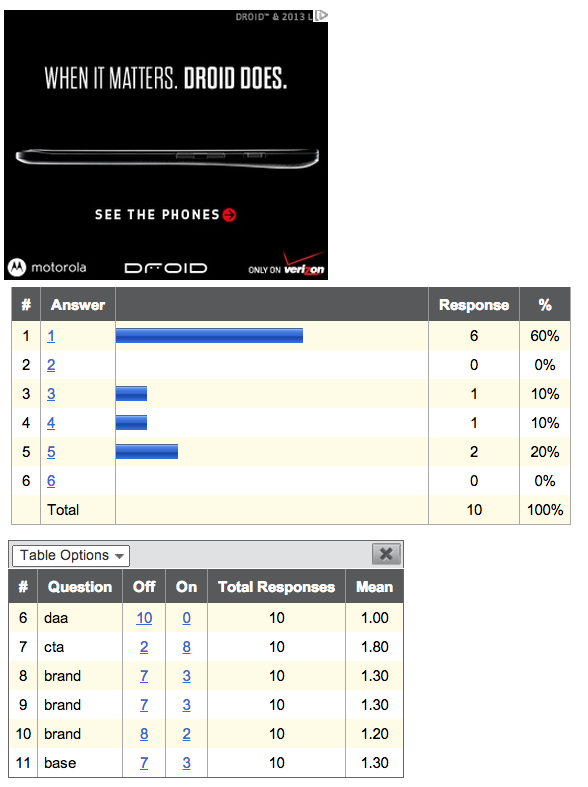
\includegraphics[scale=.3]{chapter6.tex/daa-example}
}
\caption{Android Ad with AdChoices Icon}
\label{prepilot-adchoices}
\end{figure}


Finally,  \autoref{prepilot-adchoices}  is an ad with the AdChoices icon. No one clicked on the AdChoices icon. But 8 of 10 clicked on the ``See the Phones'' call-to-action. And several each clicked on the Motorola, Droid, and Verizon brands at the bottom of the image.

By examining task 2 results, I learned that my task was too complex and it was possible participants may have mis-understood what was asked of them. However, the pre-pilot also proved the feasibility of studying user perception of the indexicality of advertisements. This simple qualitative study provided insight valuable to the design and implementation of controlled experiments.

\section{Aims}
\label{aims}

In this pilot, I consider indexical reference in hyperlinked advertisements in the context of task-based interaction. In experiment 2A I look at how knowledge contributes to perception of an indexical link on a brand icon. In experiment 2B, I look at iconic buttons on advertisements to see if the presence of a button affects where a user clicks on an ad.

\section{Experimental Design}
\label{experimentaldesign}

Study 1A considers the proposition that iconic elements of advertisements are perceived as indexical if people know what the icon represents, it contrasts semantically with the advertisement, and it signals communicative intent (for example, as a ``call-to-action''). This breaks down into to three study different hypotheses.

\begin{description}
\item{Hypothesis 2A1} \hfill \\ 
Known icons, embedded in advertisements, with brands contrastive to the background advertisement, are perceived differently than icons that semantically match the brand of the primary advertisement.
\end{description}
A McDonald's icon on a McDonald's ad should not be seen as indexical: merely iconic. However, an Apple icon on a McDonald's site might be considered indexical.
\begin{description}
\item{Hypothesis 2A2} \hfill \\
Known icons, embedded in advertisements, are perceived differently than those that are unknown.
\end{description}
This hypothesis predicts that icons which are unknown may be treated differently than those that are known. That is, a fake brand may be perceived differently than the known Apple brand. Likewise, the AdChoices icon, if unknown, should be treated as an unknown brand.
\begin{description}
\item{Hypothesis 2A3} \hfill \\
An icon that signals action is perceived differently than an icon that does not signal action.
\end{description}

A Twitter logo (as appears in \autoref{social-media}) is iconic and known to serve one of several functions: "tweet" or "go to Twitter" (to tweet/follow). Likewise, a plain FaceBook icon (also in \autoref{social-media} may be perceived to function as "share" or "go to FaceBook" (to share/follow).\footnote{These observations are made on the basis of a short AMT survey where I asked 40 turkers what they thought these icons meant in the context of the Yahoo news article in \autoref{social-media}.} That people know these things about Twitter and FaceBook is a function of their relative popularity online.  Hypothesis 2A3 predicts that icons, known or unknown, will be perceived differently if they signal action such as share/follow/post/goto, etc.

\begin{figure}
\centerline{
  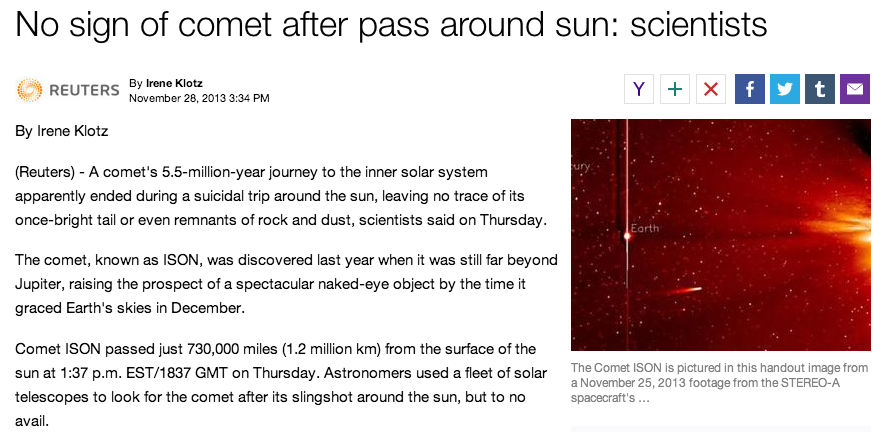
\includegraphics[scale=.3]{chapter6.tex/socialmedia}
  }
\caption{Twitter and FaceBook Icons}
\label{social-media}
\end{figure}


Experiment 2A is a single factor posttest-only design. There is one \textbf{independent variable with 5 levels}: ``same brand'', ``different brand'', ``unknown brand'', ``known signal'', and ``AdChoices''. There is one \textbf{dependent variable}: perception of an indexical reference. Five groups are required. The control group sees a McDonald's ad with an icon McDonald's logo in the upper right hand corner. Other groups see a different logo of the same size in the same place: Apple, Unknown, FaceBook, and AdChoices. Apple and FaceBook logos were chosen since they have among the highest global brand recognition  \citep{Interbrand:aa}. 
 
\begin{description}
\item{Hypothesis 2B} \hfill \\
Iconic graphical elements influence the click behavior by affecting where people click.
\end{description}

Experiment 2B is a single factor posttest-only design with three levels. The control and two treatment groups are presented with a a newspaper article containing an ad. The control group receives an ad with no ``call-to-action'', while one treatment group sees the same ad but with a textual ``call-to-action'', and the other treatment group sees the same ad with an iconic button containing the same ``call-to-action'' text as the first treatment group. The \textbf{independent variable} is ``icon'' and \textbf{dependent variable} is click location (on the ``call-to-action'' or elsewhere). 

Data for Experiment 2A and 2B were collected in separate events. Following presentation of a single task, survey data was collected.

\section{Method}
\label{method}

These two experimental designs follow the general procedure outlined in Chapter Four.

\subsection{Experiment 2A Method}
\label{experiment2amethod}

\subsubsection{Settings and Participants}
\label{settingsandparticipants}

Using Amazon's Mechanical Turk, 303 workers were paid \$0.15 to participate in one of two conditions of the single-factor design previously described. Participants were assigned randomly via Qualtrics block randomizer. Results were collected during the period of 7--14 October 2014. The task was expected to take approximately three minutes, though workers were allowed up to 10 minutes to complete.

\subsubsection{Procedure and Materials}
\label{procedureandmaterials}


The general procedure follows that described in Chapter Four. \autoref{2A-flow} gives a more detailed graphical depiction of flow.

\begin{figure}
\centerline{
\includegraphics[scale=.3]{chapter6.tex/2a-flow}
}
\caption{Experiment 2A Flow}
\label{2A-flow}
\end{figure}


Following presentation of instructions and consent form, participants were each presented one question, as illustrated in the exemplar in  \autoref{2A-adchoices},  followed by survey questions. Participants were instructed to ``Please click on things you think are links.'' 

The image used was taken from on online article at  \url{http://yahoo.com},  while the advertisement from  \url{http://moat.com}.  Alterations were accomplished using PhotoShop to create five variants. Logos were restricted to a size of approximately 20px x18px to approximate the 19px x15px (icon only with container) size specified by  \cite{Anonymous:2011ur}.  However, all logos including the AdChoices icon were presented with 100\% opacity on a white background, except for the Apple logo which was unaltered as white on a black background.


\begin{figure}
\centerline{
\includegraphics[scale=.3]{chapter6.tex/2a-daa}
}
\caption{McDonald's Ad with AdChoices Icon}
\label{2A-adchoices}
\end{figure}


\subsubsection{Instrumentation}
\label{instrumentation}

In addition to features provided by AMT and Qualtrics, my scripts performed the following:

\begin{sloppier}
\begin{enumerate}
\item Disable preview using a custom CSS class blocking Qualtrics controls
\item Check worker hash against a FireBase web service and request worker to return HIT if the hash is in the exclusion list
\item Add worker hash to FireBase
\item Submit results to AMT on completion of the Qualtrics survey
\item Hide Qualtrics hotspot regions from mouseovers
\item  Create "sticky" notes on clicks
\item  Observe whether mouseovers were detected over treatment icons
\end{enumerate}
\end{sloppier}

The last three capabilities were developed as custom code for this particular experiment. Qualtrics provides two image annotation capabilities, both of which are limited in some respect. 

The heat map annotation provided by Qualtrics used in the pre-pilot, required that the number of clicks be pre-specified by the experimenter. This is not desirable for tasks in which participants will click an arbitrary number of times. 

Instead, I used the hotspot annotation capability provided by Qualtrics. This let me create image zones to detect where a user clicks. Unfortunately, Qualtrics zones become visible when a participant mouses over a region. For the purposes of the pre-pilot and Experiment 2, I modified the Qualtrics hotspot capability in two ways: 1) never show zones; and 2) clicking creates a small sticky note so that the participant can see some evidence of click feedback at the location of the click.

\subsection{Experiment 2B Method}
\label{experiment2bmethod}

\subsubsection{Settings and Participants}
\label{settingsandparticipants}

Using Amazon's Mechanical Turk, 202 workers were paid \$0.15 to participate in one of two conditions of the single factor design previously described. Participants were assigned randomly via Qualtrics block randomizer. Results were collected between the days of 7--14 October 2013. The task was expected to take approximately three minutes, though workers were allowed up to 10 minutes to complete.

\subsubsection{Procedure and Materials}
\label{procedureandmaterials}

The general procedure follows that described in Chapter Four.  \autoref{1B-flow}  gives a more detailed graphical depiction of flow.

\begin{figure}
\centerline{
  \includegraphics[scale=.3]{chapter6.tex/2b-flow}
  }
\caption{Experiment 2B Flow}
\label{1B-flow}
\end{figure}

Following presentation of instructions and consent form, participants were presented a screen shot from a \emph{The New York Times} article with my ad substituting for the same-sized block ad in which an ad originally appeared. I used the Ford ad that had been previously used in the pre-pilot  (same as figure \autoref{prepilot-ford}).  Participants were instructed, ``pretend you are interested in getting a hybrid car. Find the Ford ad and click on it.''

\subsubsection{Instrumentation}
\label{instrumentation}

In addition to features provided by AMT and Qualtrics, my scripts performed the following:

\begin{sloppier}
\begin{enumerate}
\item Disable preview using a custom CSS class blocking Qualtrics controls
\item Add worker hash to FireBase
\item Submit results to AMT on completion of the Qualtrics survey
\end{enumerate}
\end{sloppier}

In this experiment, I used the heat map capability of Qualtrics since only one click was requested.

\section{Data Collected}
\label{datacollected}

Using G* Power 3  \citep{PowerAnalysisIntro:2012uy}  chi square goodness of fit test, for both experiments I estimated a sample size of approximately 220 was necessary in order to detect a medium effect with power of 0.95. All surveys initiated were completed: there were no known drop-outs.

Once all assignments had been completed, (as indicated on my AMT requester dashboard), I downloaded data as a single CSV (comma separated values) file from the Qualtrics website. Data was organized such that each participant's data was on its own row.

\section{Results}
\label{results}

\subsection{Experiment 2A Results}
\label{experiment2aresults}

Because the IV is categorical (binary), a non-parametric statistics is required. Strikingly, there are very few clicks on icons at all.


\begin{table}
\caption{2A Raw Clicks}
\centering
\begin{tabular}{ccc}
Clicks & Total & Icon\tabularnewline
1 & 60 & Apple\tabularnewline
2 & 59 & Unknown\tabularnewline
2 & 58 & AdChoices\tabularnewline
10 & 52 & FaceBook\tabularnewline
0 & 59 & MacDonald's\tabularnewline
\end{tabular}
\end{table}


9\% (27 of 303) of participants said they recognized the AdChoices icon, though when questioned what it meant, only 5.6\% were correct. Of the two that clicked on the AdChoices icon, one was correct and the other mistakenly believed it would link to the advertiser's page. Of 303 participants, there were 21 mouseover events over icons --- 3 (including the two that clicked) over the AdChoices icon. This means, that had the AdChoices icon been animated on mouseover, one additional person might have been alerted that the icon was meaningful.

Given relatively little data, it is difficult to come to any strong conclusion. Results suggest that the effect size was considerably smaller than anticipated. In the pre-pilot, approximately 50\% (5 of 10) clicked the Twitter icon. In this study, only 19\% of those presented with the FaceBook icon clicked on it. As a follow-up, I added a condition that simply enlarged the icon to approximately twice the size (30px x 28px). This had no effect: only 17\% (10\slash 58) presented with the larger FaceBook icon clicked on it.

I also considered that it might be possible that, despite studies showing little difference in quality of annotation with price variation, amount of pay might might be a factor. However, I ran another 200 subjects at a higher pay rate (25 cents for a 2-minute task). This also caused no change.

It is still possible, that the small number of click observations could reflect omission effects of the paid volunteer  \citep{Rush:1978tw}.  This remains un-tested.

Finally, the pre-collection focused on images in isolation.  \graffito{Committee: I will re-run this in isolation over the Holidays. I may also test both Twitter \& FB icons.} This experiment placed ads in context. It is quite possible this accounts for differences seen. Typically, linguistic judgment tasks are presented under isolated conditions where external context plays no role. However, this experiment afforded the opportunity to observe participant behavior under relatively natural conditions and was useful for this reason, if no other.

Though I created additional stimuli, due to time constraints, they were not used in this experiment. As with Experiment 1, advertisements as stimuli (and, indeed, the background newspaper itself) introduce random effects. Thus, the results presented here do not necessarily generalize across all advertisements or embedded contexts. 

\subsection{Experiment 2B Results}
\label{experiment2bresults}

 \autoref{2B-results}  presents raw frequency counts for each of the three conditions. 


\begin{table}
\caption{2B Results}
\label{2B-results}
\centering
\begin{tabular}{cccc}
 & Button & Logo & Other\tabularnewline
\cline{2-4} 
None & 0 & 2 & 64\tabularnewline
Text & 0 & 1 & 66\tabularnewline
Button & 1 & 1 & 67\tabularnewline
\end{tabular}
\end{table}


As before, because the IV is categorical (binary), a non-parametric statistics is required. Again, some cell counts were quite low and, overall, unbalanced --- so I used a Fisher's Exact Test. The p-value was equal to 1 indicating no significant difference between conditions.

As in 2A, results differed somewhat from the pre-pilot. The difference here was the title of task and payment amount, plus slight variation in the instructions. It is possible that the effect size here was simply too small to detect. A\slash B testing of ads generally involve a large number of subjects such that it might be possible to detect actual effects on behavior where none in this size study was seen. 

This task was also presented in the context of a news article and not in isolation, as had been in the pre-pilot.  \graffito{Committee: I will re-run this in isolation over the Holidays.}  As with 2A, I ran a follow-up study offering 25 cents for a shorter task. There was no effect on performance. It is possible that a larger effect size might be observed if the task were presented in isolation, rather than in context.

\chapter{Study Three: Multiparty Discourse in the Browser}
\label{studythree:multipartydiscourseinthebrowser}

Why do users feel OBA is ``creepy''? As advertisers say, OBA simply tailors ads so that users receive more relevant advertising. Granted, this involves collecting data about online activity, but consumers willingly give data to data to first-party sites all of the time. What makes this feel different?

\section{OBA is ``Creepy''}
\label{obaiscreepy}

 \cite{Ur:2012ws}  conducted semi-structured interviews with 48 non-technical users about their attitudes and understanding of OBA. As they note, these participants are not representative of the general Internet population. The researchers were interested in collecting data that would reveal mental models of ``lay people'' to better understand attitudes and behaviors. 

Here are a selection of participant comments from this study after they had viewed an instructional video on OBA:


\vspace{10pt}
"It is a little creepy... because I feel that I should get to decide what is going in and out of my computer." \citep[p. 6]{Ur:2012ws}

\vspace{10pt}

"It makes me feel very insecure. Like if this is what people can figure out about me, then what else can they get off my computer?" \citep[p. 6]{Ur:2012ws}

\vspace{10pt}

"I guess I would be more willing to do it if I had a firmer understanding of how everything worked." \citep[p. 7]{Ur:2012ws}

\vspace{10pt}
"I don't think I really noticed it... but it definitely is kind of creepy when you think about it." \citep[p. 7]{Ur:2012ws}

\vspace{10pt}
"It's kind of a creepy thought that you are being followed and monitored." \citep[p. 7]{Ur:2012ws}

\vspace{10pt}

One of the subjects, 
\begin{quote}
relating a story about how she was searching for furniture the previous night and was confused when her advertisements started to feature those items.... 'It's scary. It makes me nervous. I was thinking about it last night when I was searching for stuff. Like I thought how do they know all this, how do they keep track of this, how do they do this?' \citep[p. 7]{Ur:2012ws}
\end{quote}
\vspace{10pt}

"It makes me want to go home and delete all my cookies, but then I know that's not gonna help much. It makes me mad." \citep[p. 7]{Ur:2012ws}

\vspace{10pt}
The lay person appears to have a strong emotional response to OBA. Can a theory of social communication lend insight into why? 


\section{Related Privacy Research}
\label{relatedprivacyresearch}

What makes people willing to share sensitive information online? Behavioral economists  \citet*{Acquisti:2012tp}  find that disclosure operates under certain principles espoused by  \cite{Kahneman:1979wl} and \cite{Tversky:1981vc}. 

In an analysis of decision under risk,  \cite{Tversky:1981vc}  find that people people make choices by weighing their decisions in light of choices and perceived outcomes of competing choices. Choices are comparative:

They also find that choices depend on a starting reference point:
\begin{quote}
An essential feature of the present theory is that the carriers of value are 
changes in wealth or welfare, rather than final states. This assumption is compatible with basic principles of perception and judgment. Our perceptual apparatus is attuned to the evaluation of changes or differences rather than to the evaluation of absolute magnitudes. When we respond to attributes such as brightness, loudness, or temperature, the past and present context of experience defines an adaptation level, or reference point, and stimuli are perceived in relation to this reference point. \citep[p. 277]{Kahneman:1979wl}
\end{quote}

 \cite{Acquisti:2012tp}  focus on the notion of a changing reference point in order to see what sorts of signals might affect a respondents willingness to disclose sensitive information. They do so by measuring people's propensity to admit to engaging in sensitive (embarrassing, unethical, and illegal behavior) in a series of surveys.

They find evidence that people will admit to having engaged in sensitive behaviors when they are lead to believe that others have admitted in similar behaviors (\emph{herding effect}). They also examine the effect of question order on disclosure (\emph{ordering effect}). And indeed it does. Participants in the increasing conditional were less likely to admit behaviors than in the condition where questions decreased started as very sensitive and then decreased in sensitivity. Both experiments support  \cite{Kahneman:1979wl}  and also give insight into how and why people disclose information online.

In a study related to  \cite{Acquisti:2012tp}, \cite{John:2009wg}  manipulated the saliency of privacy to see whether this would affect propensity to disclose. When saliency of privacy was high, willingness to admit to engaging in sensitive behaviors decreased. And when subjects were distracted from privacy concerns, their propensity to disclose was increased.

Timing also has an effect on behavior.  \citet*{Egelman:2009ut}  studied the effect of the presentation of privacy information in the context of purchase decisions. By controlling the placement, timing, and privacy level on several consumer websites during a purchase task, participants reacted differently for the purchase of privacy-sensitive items than for items with minimal privacy concerns. In four conditions, different privacy icons were used to study both when and how icon presence affects behavior.  \citet{Egelman:2009ut}  found that 1) the presence of privacy indicators influenced purchase decisions, and 2) online shoppers who were less privacy-aware, paid significantly more for privacy when privacy indicators were presented \emph{before} visiting websites than \emph{after} they arrived at the website.

Clearly, people are willingly disclose sensitive information online every day. And they are also sensitive to the presence of visual indicators that indicate degree of privacy. In the next section, I show that behavior is also affected by knowledge of the presence of external participants in interaction.

\section{Related Linguistic Resesarch}
\label{relatedlinguisticresesarch}

\subsection{The Stateful Web}
\label{thestatefulweb}

When Tim Berners-Lee first implemented the Hypertext Transfer Protocol (HTTP) in 1990, it was to facilitate communication between a client and a server on the Internet  \citep{Thewebsiteofthew:vo}.  HTTP functioned as a protocol to facilitate communication much as the telephone: it provided the means for a client to request information from a server via a small set of verbs such as ``GET'' or ``POST''. As a protocol, HTTP is stateless and does not require the server to track state between connections. This means, if a user requests a webpage that includes a number of embedded assets (e.g., images), the web server does not have to know anything about these assets nor does it have to track the status of those requests. In response to a request, a server generally replies with a status such as OK plus information about what sort of content is to be transferred followed by that content. In fact, an HTTP and response look something like this:

\begin{lstlisting}[numbers=none]
GET /
Accept-Encoding: gzip
User-Agent: Rested 2.3 (Macintosh; Mac OS X 10.8.0; en_US) 
---blank line---
\end{lstlisting}

And a response looks something like this:

\begin{lstlisting}[numbers=none]
HTTP/1.1 200 OK
Server: gws
Set-Cookie: PREF=ID=00a5929d47bf3487:FF=0:TM=1350849438:LM=1350849438:S=YYHqxKmLxevdwbvo; expires=Tue, 21-Oct-2014 19:57:18 GMT; path=/; domain=.google.com, NID=65=hS0s8SoRDwlN1gqEDi3Mx_rjCNUBddfp2ouOmMn4OGQBBV9VEejtxOuKKaIDFt5TMyrBs0ZGBZ3BH-449m2GtPjqxVsYXjuN96DgxaOybcNHfOjXwe2R9t6G05z3Hqhd; expires=Mon, 22-Apr-2013 19:57:18 GMT; path=/; domain=.google.com; HttpOnly
Content-Type: text/html; charset=ISO-8859-1
Transfer-Encoding: Identity
P3P: CP="This is not a P3P policy! See http://www.google.com/support/accounts/bin/answer.py?hl=en&answer=151657 for more info."
Date: Sun, 21 Oct 2012 19:57:18 GMT
X-Frame-Options: SAMEORIGIN
X-XSS-Protection: 1; mode=block
Cache-Control: private, max-age=0
Expires: -1
---blank line---
---HTML entity here---
\end{lstlisting}

In order to accommodate stateful applications --- applications that remember information about previous transactions, a small piece of data called a cookie can be attached to an HTTP request and deposited in the client web browser. This concept, envisioned by Lou Montulli of Netscape in 1994, was invented to facilitate a simple sort of memory  \citep{Schwartz:2001uk}.  In so doing, it also enabled the sense of dialogue between server and client. Originally, cookies were intended to support basic dialogue between user and website publisher for simple transactions such as those needed to support online shopping (e.g., a cookie can be used to keep track of a user's session to include items in a shopping cart).

Though the purpose of cookies was to support the need for state between HTTP transactions, this very simple concept fostered economic and social revolution on the Web: it fundamentally changed interaction on the web from \emph{private} to \emph{public}. Content providers found that sites could be supported by advertising revenue simply because an advertiser with an advertising server could use cookies to decide what ad to return in response to an HTTP request. Thus, in any web page transaction, tailored advertiser content could be presented alongside publisher content.

\subsection{A Model of MultiParty Interaction}
\label{amodelofmultipartyinteraction}


\begin{sloppier}
The client-server interaction described above is a sort of computer-mediated communication between humans. HTTP as a machine-based communications protocol enables two parties to exchange messages. Because messages are typically simple HTTP requests with textual or other media content as a response, there is no sense of shared social context involved between a user and web provider and such dialogues are not been of linguistic interest. On the other hand, linguistic analyses of machine mediated human conversation that occur in chat rooms, texting, weblogs, etc. are a vibrant area of study in peer-review venues such as language@internet\footnote{\url{http://www.languageatinternet.org/}}.
\end{sloppier}


Though traditionally, the term discourse has been associated with written and spoken communication, early sociolinguists such as  \cite{Hymes:1974wr}, \cite{Gumperz:1982tc}, \cite{Goffman:1981tm}, \cite{Garfinkel:1967vn}  and others have extended our understanding of discourse causing us to re-consider boundaries between linguistic and non-linguistic phenomenon in social discourse. 

As such, the main objects of study in sociolinguist approaches to discourse analysis are \emph{communicative signs and their patterning}  \citep{Gumperz:1982tc}.  Dell Hymes argues that it is not language that is fundamental in discourse, but society.

\begin{quote}
One must take as context a community, or network of persons, investigating its communicative activities as a whole, so that any use of channel and code takes its place as part of the resources upon which the members draw. \citep[p. 4]{Hymes:1974wr} 
\end{quote}
Furthermore, 
\begin{quote}
It is [...] not linguistics, but ethnography, not language, but communication, which must provide the frame of reference within which the place of language and culture is to be assessed. \citep[p. 4]{Hymes:1974wr}
\end{quote}
\begin{sloppier}
When considering Internet communication, it matters little whether particular interactions are "conversational" --- whether responding on a forum, or requesting an article from the New York Times, or "liking" a photo, or requesting an arbitrary web page. What matters is the context; what matters is that \textbf{web interaction supports a paradigm of multi-party communication}. 
\end{sloppier}

The web is now a very public medium in which interactions between particular persons --- or between a user and publisher --- occur in a virtual space occupied by many other simultaneous participants. Though web interaction may feel very personal while sitting at ones desk at home, it is as public as conversing in a cocktail party. Moreover, interaction with a particular web site can feel very much as a private dialogue where one meets again and again to continue interacting as if no absence has occurred between  sessions.\footnote{The hidden nature of personalization is a fascinating, related area of interest. In 2011, Eli Pariser wrote a book on the topic entitled \textit{The Filter Bubble: What the Internet is Hiding from You} in which he describes how data mining algorithms are largely responsible for a very personalized experience on the web that influences everything from search results to whose activity is seen on Facebook.} 

\subsection{Modeling the Hearer}
\label{modelingthehearer}


Though conversation has more generally been described in dyadic (two-party) models, several notable sociolinguists have touched upon multi-party conversation and distinguished between hearer / listener roles \citep{Hymes:1974wr, Goffman:1981tm, Bell:1984tx, Levinson:1988wt, Clark:1982tg, Schober:1989wn, Clark:1987wh, Clark:1992ty, Clark:1996tm}. \citet{Dynel:2010th} has attempted to reconcile these various classifications into a unified hearer model. In part, the need to do so stems from the analyses of new forms of discourse, such as radio, television dramas, etc. 

\cite{Goffman:1981tm} first divided hearers into two categories: ratified and unratified.\footnote{\cite{Levinson:1983ww}, following \cite{SantaCruzlectures:1971te}, refers to authorized speakers and authorized recipients.} Ratified hearers are those "entitled to listen to the speaker" whereas unratified are non-official participants, such as bystanders, who are present but not addressed. Ratified participants include the speaker, addressee and other "official hearers" (e.g., "third parties")\footnote{Note overlapping terminology with "third party" used in a legal sense. Superficially, these appear to have the same meaning. However, behaviorally, third parties in online tracking act may across a range of hearer / listener roles.} who are expected to follow the conversation but who are not addressed. \cite{Bell:1984tx} and \cite{Clark:1992ty} further distinguish unratified hearers as "bystanders" and "eavesdroppers". The primary distinction between "bystander" and "eavesdropper" is that the \textit{speaker is aware of the presence of bystander and capacity to overhear}. \citep{Dynel:2010th, Clark:1992ty}. See \autoref{participants} for a graphical representation of Dynel's \citeyearpar{Dynel:2011fd} synthesized model.

\begin{figure}
\centerline{
\includegraphics[scale=.75]{chapter7.tex/participants}
}
\caption{Modeling Hearers in Discourse (Adapted from  \citealp{Dynel:2010th})}
\label{participants}
\end{figure}

\begin{sloppier}
The distinction between bystanders and eavesdroppers serves an important distinction with respect to how speakers communicate. When the speaker is aware of a bystander, she can adjust her utterance in a number of ways. In dealing with overhearers, speakers  estimate how much the overhearer can infer; then design their utterances, accordingly \citep{Clark:1992ty}. 
\end{sloppier}

With respect to a shared common ground, there are two sorts of information that the speaker must consider. \textit{Open information} is information that overhearer believes or could readily guess to be in the common ground. \textit{Closed information} is information that the overhearer doesn't believe, and could not readily guess to be in the common ground \citep{Clark:1992ty}. It is the discrepancy between these two sorts of information that may be exploited by the speaker to affect what an overhearer (bystander or eavesdropper) might conjecture \citep{Clark:1992ty}. 

\begin{sloppier}
There are four main attitudes that a speaker can take toward overhearers: \textbf{indifference} (the speaker doesn't care whether the overhearer understands what she is saying or not), \textbf{disclosure} (the speaker tries to provide enough information that the overhearer can infer the right meaning), \textbf{concealment} (the speaker tries to deprive the overhearer of enough information to correctly infer what is meant --- e.g., you-know-who did you-know-what to whom), and \textbf{disguisement} (the speaker attempts to conceal her meaning from the observer while also deliberately mis-representing that meaning; \citep{Clark:1992ty}. 

Thus, \textbf{audience design} can be divided roughly into addressee design, third party design, and overhearer design \citep{Clark:1982tg}. It's worth noting that participant roles are constantly negotiated between interlocutors according to regular (e.g., turn-taking) procedures. And as \cite{Dynel:2010th} notes, one role may be performed by a number of individuals simultaneously.
\end{sloppier}

Online tracking represents a sort of discourse where the primary participants are a user interacting with a particular web site --- which has a participant role represented by a company or organization. Other hearers are present. Perhaps, ratified and perhaps not. When overhearers are not ratified, their understanding is not grounded. What they understand is conjecture. Sometimes what they may understand may be the same as a ratified hearer, and sometimes not. In an experiment conducted by \cite{Schober:1989wn}, ratified hearers were able to match understanding with the speaker with a very high degree of success. But despite the speaker and hearer deliberately obfuscating their speech in the presence of an overhearer, overhearers were still successful some of the time. More importantly, overhearers were also sometimes wrong.


\section{Aims}
\label{aims}

In this pilot, I consider whether experiment participants view advertisers as bystanders or eavesdroppers. To do this, I compare behavior across two conditions: subjects in the control condition answer a series of sensitive questions. In the treatment conditions, subjects perform the same task but are presented with visible evidence of advertisers as bystanders. This follows the general experiment design of  \citep{Acquisti:2012tp}  but poses a new dependent variable for investigation: \emph{visual presence}.

\section{Experimental Design}
\label{experimentaldesign}

This study has one experimental hypothesis:

\begin{description}
\item{Hypothesis 3} \hfill \\
People answering sensitive questions will behave differently in the presence of unratified participants than when simply notified in advance about the possibility of unratified participants.
\end{description}

In this \textbf{between} group, \textbf{single-factor}, \textbf{repeated measures} posttest-only design, the control group is asked to respond to a survey containing questions relating to sensitive activities (using questions drawn from  \citep{Acquisti:2012tp}).  Participants are notified in a privacy statement that there may be ad trackers on the site. The treatment group receives exactly the same notification and survey. However, tracker presence is indicated in a visual display throughout the participant's session. 

There is one \textbf{independent variable}: ``visual presence''. The \textbf{dependent variable} is the propensity to respond in affirmative to engaging in specific behaviors. This represents the willingness to divulge sensitive information under circumstances which may appear to be more or less private. 

Following presentation of stimuli, survey data is collected for both experimental designs. 

\section{Method}
\label{method}

This experimental design follow the general procedure outlined in Chapter Four.

\subsection{Settings and Participants}
\label{settingsandparticipants}

Using Amazon's Mechanical Turk, 213 workers were paid \$0.15 to participate in one of two conditions of the single-factor design previously described. Participants were assigned randomly via Qualtrics block randomizer. Results were collected during the period of 7--14 October 2014. The task was expected to take approximately three minutes, though workers were allowed up to 10 minutes to complete.

\subsection{Procedure and Materials}
\label{procedureandmaterials}

The general procedure follows that described in Chapter Four.  \autoref{3-flow}  is a more detailed graphical depiction of flow.

\begin{figure}
\centerline{
  \includegraphics[scale=.3]{chapter7.tex/exp3-flow}
  }
\caption{Experiment 3 Flow}
\label{3-flow}
\end{figure}

Following presentation of instructions and consent form, participants were each presented the following six question in the order given.

\begin{enumerate}
\item Have you bounced a check?
\item Have you cheated on a tax return?
\item Have you made a false or even somewhat inflated insurance claim?
\item While an adult, have you had sexual desires for a minor?
\item Have you had sex with the current husband, wife, or partner of a friend?
\item Have you fantasized about having violent, non-consensual sex with someone?
\end{enumerate}

Possible answers were:

\begin{enumerate}
\item Never
\item Once or twice
\item Sometimes
\item Frequently
\end{enumerate} 

As in  \cite{Acquisti:2012tp},  propensity to disclose is indicated by a positive answer. All positive answers are combined into a single score. Non-answers (skipped questions) count as non-disclosure. Thus, the dependent variable is binary.

\subsection{Instrumentation}
\label{instrumentation}

In addition to features provided by AMT and Qualtrics, my scripts performed the following:

\begin{sloppier}
\begin{enumerate}
\item Disable preview using a custom CSS class blocking Qualtrics controls
\item Check worker hash against a FireBase web service and request worker to return HIT if the hash is in the exclusion list
\item Add worker hash to FireBase
\item Submit results to AMT on completion of the Qualtrics survey
\end{enumerate}
\end{sloppier}

No other instrumentation was required for this experimental design.

\section{Data Collected}
\label{datacollected}

Using a G* Power 3 f-test for linear multiple regression with a fixed model, I estimated a sample size of approximately 89 was necessary in order to detect a medium effect with power of 0.95. All surveys initiated were completed: there were no known drop-outs.

Once all assignments had been completed, (as indicated on my AMT requester dashboard), I downloaded data as a single CSV (comma separated values) file from the Qualtrics website. Data was organized such that each participant's data is on its own row.

\section{Results}
\label{results}

There is some difference in the demographic profile between the Experiment 3 sample and the  \citet{Acquisti:2012tp}  sample. That study reported a mean age of 40, 45\% male, and 82\% caucasian. This study was 63\% male, 82\% caucasian, 68\% under 35, and, likely, with lower income levels (given NYT has a subscription fee for regular readers): 53\% reportedly make below 30K. Regardless, comparing control group responses from  \cite{Acquisti:2012tp}  with control group responses here, propensity to disclose was very similar.

Interestingly, the percentage of male respondents for Experiment 3 was higher than the aggregate population studied across all experiments in this dissertation  (63\% versus 53\%; see \autoref{survey-response}).  This suggests that some population of workers, including females, elected not to participate in this study. I will come back to this point in a bit.

 \autoref{3-raw}  below presents averages across all six questions. A simple chi-square test reveals no difference between groups  (p = 1).\footnote{This is with and without a bonferroni adjustment for repeated questions (p = .046)} 


\begin{table}
\caption{Raw Results (Aggregate Mean)}
\label{3-raw}
\centering
\begin{tabular}{ccc}
\hline 
 & Control & Treatment\tabularnewline
\hline 
Never & 41.33 & 42.17\tabularnewline
Once or twice & 6.83 & 7.00\tabularnewline
Sometimes & 2.33 & 1.33\tabularnewline
Frequently & .50 & .50\tabularnewline
\end{tabular}\end{table}


There are two factors that may account for observed differences between this study and  \citet{Acquisti:2012tp}.  First, the population sampled here is surprisingly sensitive to privacy issues. Moreover, AMT as a platform is not seen as anonymous --- as the  \citet{Acquisti:2012tp}  survey may have been perceived. The mere fact that I presented an IRB form with names and contact information affected discourse context.

Second, answering specific questions in the  \cite{Acquisti:2012tp}  survey was completely voluntary; `no answer' accounted for between roughly 10--15\% for each question asked. This was calculated in the metric for propensity to disclose.

Selectional differences in this study are reflected in a couple of ways.

\begin{itemize}
 \item \textbf{Population Bias.} There is no way to know if the people who elected not to participate in Experiment 3 did so because they did not want to see "sensitive" questions or because they were concerned with privacy. Regardless, there is a population bias --- as reflected by the relative gender disparity between Experiment 3 and aggregate demographics across all five studies.
\item \textbf{Obligation.} No one in this experiment tried \textit{not} to answer a question. This may relate to the nature of the obligation workers feel to requesters as paid subjects. 
\end{itemize}


Over the course of the past two years, tremendous change has occurred on the Internet. Savvy users, like those found on AMT, are well aware that what they say and do may be monitored. One of my participants noted in comment, ``nothing is private online now due to the NSA.'' Events have conspired to raise the saliency of privacy issues on the Internet for even casual Internet users. Despite this, my survey reveals perceptual differences for feelings of privacy on the Internet whether connected at home or in a public setting. \autoref{privacy}  represents answers to the following two questions:

\begin{enumerate}
\item How private do you feel on the Internet when you are using your computer (laptop, or tablet) in public. Public means something like a coffee shop, library, school, etc.
\item How private do you feel on the Internet when you are using your computer (laptop, or tablet) at home?
\end{enumerate}

\begin{figure}
\centerline{
\includegraphics[scale=.5]{chapter7.tex/exp3-graph}
}
\caption{Feelings of Privacy on the Internet in Public and at Home}
\label{privacy}
\end{figure}

It's clear that physical setting, at least, lends some expectation of privacy whether one is on the Internet on a personal machine at home or in public. Though visual saliency was not a factor in propensity to disclose in this experiment, users have an expectation of privacy when they are not in a public setting. Given the Internet is now ``public'', there exists some mis-match of expectation that is not accounted for in Internet browser design.

\chapter{Discussion}
\label{discussion}

This thesis presents the argument that discourse understanding 1) shapes how people understand and interact with graphical user interfaces on the Internet; and 2) how such knowledge might be used to manipulate context, affecting comprehension and, therefore, behavior.

By analyzing GUI microinteractions in the way that we analyze linguistic discourse, it may be possible to explain some sorts of mis-understandings and even present solutions for improving user interaction design. This chapter summarizes results of experiments from the previous three chapters in context of related work in cognitive science.

While qualitative methods are extremely important for guiding a research program, it is through quantitative methods that causality is determined. While Experiments 1 and 2 focused on user comprehension, Experiment 3 concerned how knowledge about the presence of third-parties affects production. The third experiment was problematic in several respects.

\section{Summary of Findings}
\label{summaryoffindings}

 \autoref{summary-results}  summarizes results for all experiments in this dissertation.


%% LyX 2.0.6 created this file.  For more info, see http://www.lyx.org/.
%% Do not edit unless you really know what you are doing.
%\documentclass[english]{article}
%\usepackage[T1]{fontenc}
%\usepackage[latin9]{inputenc}

%\makeatletter

%%%%%%%%%%%%%%%%%%%%%%%%%%%%%% LyX specific LaTeX commands.
%% Because html converters don't know tabularnewline
%\providecommand{\tabularnewline}{\\}

%\makeatother

%\usepackage{babel}
%\begin{document}
%B%
%\begin{table}
%\begin{center}
\begin{longtable}{l p{10cm}}
\caption{Experiment Design} \\
1A & 2x2x2 between group posttest-only design where the control group is
presented with a set of textual expressions and asked to answer
questions about their meaning. Treatment groups are presented with either textual expressions or a dialog box expressing the same set of choices and asked the same
questions. Independent Variables: Modality, Deontic force, Attitude
toward privacy. Dependent Variable: Pragmatic implicature\tabularnewline
\hline 
1B & Between group posttest-only design where two groups are presented
with a cookie banner and later asked about whether or not they believe
the website placed \textquotedbl{}cookies\textquotedbl{} in their
browser. The treatment group is presented with feedback about the
consequence of their action / non-action following presentation of
the banner. Independent Variable: Feedback. Dependent Variable: Pragmatic
implicature.\tabularnewline
\hline 
2A & Between group posttest-only design where five groups are presented
an advertisement in the context of a webpage and asked to identify
hyperlinks. Treatment groups are presented an advertisement with embedded
image icons at four levels (known icon + different company, unknown icon, known call-to-action (CTA), ``DAA opt-out icon'') while the control group is presented with an embedded image from the same company as the advertiser. Independent
Variable: Icon type. Dependent Variable: Indexicality of icon. \tabularnewline
\hline 
2B & Between groups posttest-only design where three groups are presented
an advertisement in the context of a webpage and asked to identify
hyperlinks. Treatment groups are presented an advertisement at two
levels (iconic CTA, textual CTA) while the control group is presented
with an advertisement with no CTA. Independent Variable: Modality
of CTA. Dependent Variable: Click target.\tabularnewline
\hline 
3 & Between group repeated measures posttest-only design where a control
group is asked to respond to a survey containing questions relating
to activities (using questions drawn from \cite*{Acquisti:2012tp}; embarrassing, socially / ethically questionable, illegal). Participants
are notified in a privacy statement that there may be ad trackers
on the site. The treatment group receives exactly the same notification
and survey. However, tracker presence is indicated in a visual display
throughout the participant's session. Independent Variable: Visual
presence. Dependent Variable: Propensity to respond in the affirmative
to engaging in specific behaviors.\tabularnewline
\hline 
\end{longtable}
%\end{center}
%\end{table}
%\end{document}



\section{Discussion of Results}
\label{discussionofresults}

Pragmatic theory distinguishes between several types of factors affecting comprehension and reasoning:

\begin{enumerate}
\item \emph{Social dimensions} of discourse (e.g., cooperative principle; intent; norms; participant roles)

\item \emph{Knowledge} (e.g., subject \slash  content matter; deictic relations)

\item \emph{Saliency} (e.g., cognitive saliency of referents; task saliency)

\end{enumerate}

Attitudes and beliefs also affect reasoning as described by  \citet{Kahneman:1984td},  though these do not fall under the purview of pragmatic theory.

Experiment 1 concerned pragmatic reasoning where subjects reasoned over both textual and mixed-modal content. Not only were mixed-modal representations subject to the same sorts of pragmatic inferences as purely textual representations, small changes in language and content were shown to have significant effect in understanding and, ultimately, behavior. Furthermore, immediate feedback was seen to affect comprehension. 

Experiment 2 primarily considered the role of knowledge (icon referent) in the inference of an indexical relation. By manipulating an icon embedded in a graphical ad, I looked at whether knowledge about that icon (against a background context) played a role in its interpretation. In the pilot, it seemed this was the case, but in the actual experiment, any effect was too small to see. The primary difference was that in Experiments 2A and 2B, the ad image was embedded in the larger context of a news article while in the pre-pilot, the ad was considered in isolation.

Finally, Experiment 3 concerned whether manipulation of visual presence (and, therefore, participant role) would affect responses in a task measuring propensity to disclose sensitive information. In theory, this should be the case. However, I believe elements of task context (including use of AMT) and user knowledge may have affected results.

Below I discuss each experiment in more detail.

\subsection{Experiment 1: Modal Dialog Boxes}
\label{experiment1:modaldialogboxes}

Assuming a common set of principles driving understanding of both multimodal and textual content, people should be as sensitive to implicature in multimodal messages as linguistic messages. In fact, it appears not only is this so, but to a higher degree. This has clear implication for design: \emph{user choices made using non-forced choice modal dialog boxes may be mis-understood}.

Why might people mis-understand the meaning and consequence of choice?

 \citet{Evans:2003gp}  asserts evidence for two types of thought processes: \emph{heuristic} and \emph{analytic} (also referred to as System 1 and System 2, as well as, Type 1 and Type 2 in  \citealp{Kahneman:2011tc,Manktelow:2012tx}, respectively).  Much of this work is based on studies of deductive reasoning. For example, the Wason selection task  (\autoref{wason}; \citealp{Wason:1960wt})  asked people to select cards which falsify the statement in (a). Subjects were shown 4 cards and told that each card had a letter on one side and a number on the other. The correct answer is A and 7, though only 10--20\% of people answered correctly  \citep{Wason:1960wt}.  However, when given task (b) and told they play the role of a police officer checking people drinking in a bar, about 75\% were successful  \citep{griggs1982elusive}.  

These studies and others, point to a belief bias where belief is seen to affect reasoning about logical arguments. Similarly, a matching bias is seen in more abstract tasks; a matching bias is one in which one tends to select answers which contain lexical content which matches content over which one is reasoning (e.g., selection of A and 3 as answers in the Wason task mentioned earlier). Such biases provide support for a heuristic, autonomous system for reasoning which takes into account knowledge and belief. Other processes relating to the social dimensions of language use, also appear to be automatic (discussed in the next section).

There are several theories of reasoning that aim to explain this sort of phenomenon:  \citet{Cheng:1985ww}  propose domain specific knowledge structures (pragmatic reasoning schemes) which are remembered and applied from previous experience to new situations;  \citep{JohnsonLaird:1983vt}  argues that people create mental models of assertions and rely on these to reason; and,  \citep{Cosmides:1989dq}  proposes a ``social contract'' algorithm which is specialized to assess costs and benefits in social exchange.


\begin{figure}
\centerline{
  \includegraphics[scale=.75]{chapter8.tex/wason}
  }
\caption{Wason Selection Task (Image credit: \citealp{Evans:2003gp})}
\label{wason}
\end{figure}


Whether through discourse models, pragmatic reasoning schemas (PRS), or other heuristics, people are adept at reasoning over discourse with little apparent effort or thought. In all conditions, subjects were subject to implicature (see  \autoref{exp1-raw}  for raw results). What is surprising is how sensitive implicature is to small changes context. Across eight conditions, interpretation of implicature varied from 38\% (text, pictures, on\slash off) to 84\% (graphics, cookies, on\slash off). 

Experiment 1B was concerned with how people interpret the question presented in Experiment 1A --- but in the context of decision-making. In Experiment 1A, subjects were asked what they thought `cancel' or `x' meant. They had time to reflect and reason. 

In Experiment 1B, subjects were asked to think about what they thought their choice meant immediately after making a decision. Surprisingly, a great number of subjects attended to the dialog box and chose to respond (30--35\%). This is likely a higher percentage than what might be expected of the population of users on the Internet as a whole. Only 22\% of those in the control condition made an inference about the presence of cookies based on their choice. Of those that didn't, 45\% of those that thought there were cookies answered ``there are probably always cookies'' and 72\% of those who didn't think there were cookies said they used an ad blocker. The large number of turkers who believed there were always cookies suggests a belief bias. And the number that used ad blockers strengthens this: turkers are very knowledgeable of privacy issues.

Of those that did interpret an implicature, it's possible a matching bias was in effect. It is also possible subjects short-cut reasoning using a simple schema or model. Either way, subjects may have reasoned:

\begin{itemize}
\item "I didn't select NO and I didn't select YES, therefore neither NO nor YES." 
\item Or, perhaps, "I didn't select NO, therefore YES." 
\item Or, similarly, "I didn't select YES, therefore NO."
\end{itemize}

Why one would select one or the other of the latter two is a good question. Either way, they made a choice without understanding the consequence.

The number of people making an inference about the presence or absence of cookies based on choice was lower than expected. The high ``participation'' for choice seems likely due to the nature of the task environment: workers may be likely to cooperate and take action on prompts because they have agreed to do work for pay. 

Regardless, there were far fewer inferences made when feedback was provided. \emph{Without immediate feedback, odds were 6.6 times higher that subjects understood an implicature to be true}.

\subsection{Experiment 2: Embedded Icons in Graphical Ads}
\label{experiment2:embeddediconsingraphicalads}

Experiment 2 was also about pragmatic reasoning, though not the sort associated with logical or semantic reasoning. In the pre-pilot to Experiment 2, participants examined advertisements and were asked to click wherever they thought there might be a hyperlink. Hyperlinks associate an object on a page or in a scene with other content. When there are no visual cues, such a relation largely derives from knowledge people have about the meaning of an object and to what it might refer. Even so, judgements seems to be context sensitive.

In Experiments 2A and 2B, participants were given a task in context --- advertisements were embedded in a news page. From Experiment 2A, it seems that an icon embedded in a graphical advertisement is not likely to be considered indexical, regardless of what that icon represents --- except in the case of the FaceBook icon which is an explicit ``call-to-action'' (like \slash  share) associated with all sorts of different content on the Internet. I had hypothesized that several factors might be at play: 1) icon salience by a contrastive relation (visually \slash  semantically) with the background ad; 2) knowledge that the icon is indexical to some brand; and, 3) recognition of a signal or ``call to action'' for clicking. In 2A, the only icon which was considered indexical was the FaceBook icon, exhibiting all three properties. It is possible that estimating for a medium effect size for an ad in context, was not enough to see whether (1) and (2) made a difference, independently.

Experiment 2B attempted to determine whether explicit indexicality affected behavior. Would an ad with a CTA that had the form of a button invite a user to click directly on the button? In the pre-pilot, this appeared to be the case, but there was no effect in the embedded context of Experiment 2B. Again, it is possible that the embedding context (ad within a news page) had an effect, potentially reducing the effect size. It is also possible that we may see no effect with more savvy Internet users but would see one with those who are less savvy.

Regardless, these insights were useful in understanding why the AdChoices icon may not be effective for conveying intent to users. Size has less of an effect than one would imagine. More important, \emph{embedded graphics in ads may not be considered indexical by default}. At least not today. As users become accustomed to certain associations and patterns, they may well adapt.

\subsection{Experiment 3: Third-Party Bystanders Versus Eavesdroppers}
\label{experiment3:third-partybystandersversuseavesdroppers}

Experiment 3 attempted to address whether participants might change their behavior depending on whether they thought advertisers were actively observing them (i.e., the difference between non-ratified bystanders versus non-ratified, eavesdroppers). If the treatment group behaved differently, this would lend support to the notion that participants aware of being monitored, changed their behavior in response. However, it appears that both groups were equally cognizant of the potential for third-party monitoring. 

Two years ago, turkers, along with most people on the Internet, had little knowledge of OBA. In a recent survey conducted by  \citet{Lease:2013vq},  at least some AMT workers were aware of the potential for leakage of personal identity via workerId: worker identity is not completely private and can be found in web searches. The survey in this dissertation revealed that more than 90\% of turkers knew what cookies were, and what's more, nearly 75\% used ad blockers. Though most of them felt ``more private'' on the Internet at home than when sitting in a public setting, they seem to have a heightened sensitivity toward privacy issues which may have affected the outcome of this experiment.

Video gaming site owner, Niero Gonzalez was surprised to find that nearly have of his 3 million visiter a month blocked ads  \citep{Hill:2013wp}.  From the same source, PageFair says that ad blocking is growing at a rate of 43\% per year. Given how knowledgeable my sample was about Internet privacy and tracking technology, few would consider their communications anonymous. Moreover, given the contractual relation between the requester and worker on AMT, only those willing to share sensitive information would be willing to accept such a HIT. Quite possibly, this rendered the question of bystanders versus eavesdroppers irrelevant.

 \citet{Ur:2012ws}  deliberately recruited non-technical people who were little aware of tracking on the Internet. By contrast, turkers are very aware of tracking. Perhaps, results would have been different two years ago. In Experiment 3, the sample studied was likely not representative of the larger population of Internet users. From this perspective, AMT was not a suitable recruitment platform. However, turkers may reflect what we will see from the majority of users in time. And, good or bad, what feels creepy now, may not after longer familiarity.

\subsection{Use of AMT}
\label{useofamt}

Only recently have researchers in pragmatics and sociolinguistics adopted controlled experimentation (and on platforms such as Mechanical Turk) for the study of discourse phenomena.  \citet{Assessingthepragma:2011ug}  note that pragmatic phenomena are difficult to study because of the many contextual parameters that affect understanding. Crowdsourcing platforms such as AMT now make it possible to vary context parametrically without excessive expense and time. In a study of scalar implicature,  \citet{Assessingthepragma:2011ug}  found that simply changing the task instructions to ``quality control'' altered the proportion of responses in an implicature-oriented situation. Though such methods look useful for testing UI design comprehension, there is much to learn about how to best do this.

\subsection{Potential Population Bias}
\label{potentialpopulationbias}

In both methods and presentation of experiment results, I've noted attributes or characteristics of the AMT population that makes it difficult to typify them as characteristic, non-privacy aware Internet users. Other potential issues, regarding use in cognitive and other experiments were also noted. Like other researchers, I performed tests varying payment looking for quality differences across collection events. However, differences between results in Experiment 2 pre-pilot and Experiments 1 \& 2 suggest that there may be another factor.

 \citet{Rush:1978tw}  noted that subjects that volunteer for pay tend to commit more errors of omission on selective attention tasks. They suggested that paid subjects might working more for task completion than success. In experiment 2B, I offered a 3-minute task for 15 cents. Even when I added collection events increasing payment to 25 cents, and shortening the task by omitting demographic questions, I saw no difference in results. Yet, corresponding samples from the pre-pilot at 75 cents (15--20 minute task) obtained different results. It also possible some other variable might be in play. Perhaps, some workers (e.g., those focused on pay) simply prefer more attractive tasks (easiest; highest reward to time ratio). These tasks are consumed quickly leaving ``less attractive'' tasks for other turkers to tackle. This question remains future work.

\section{Cognitive Architecture}
\label{cognitivearchitecture}

As central goal of this dissertation is to provide support for the notion that user interaction with graphical user interfaces involves discourse processes, a basic discussion of the cognitive architecture facilitating language understanding is essential.

\subsection{Situation Models}
\label{situationmodels}

Language, perception, and action are closely aligned  \citep{Lakoff:2008tq}.  In recent years there has been much support from brain imaging. For example,

\begin{itemize}
\item Activity in pre-motor cortex suggests a causal link for the understanding of action verbs \citep{Willems:2011gp};
\item High manipulability words evoke greater activation in the motor cortex \citep{Madan:2012ja};
\item Perspective in pictures has an effect of learning \citep{deNooijer:2013jc};
\item Evidence of the activation of modality specific representations during discourse show that mental imagery occurs during discourse comprehension.\citep{Kurby:2013tp}
\end{itemize}

Furthermore, theories of language comprehension suggest that text comprehension involves the constructions of a mental representation of events described in text  \citep{Zwaan:2002va,Kintsch:1978vz,vanDijk:1990tc}.  

In semantics, a propositional representation conveys logical meaning using lexical and grammatical features. Depictive representations, on the other hand, do not encode such relations symbolically. Propositional and depictive representations make different sorts of information explicit and accessible  \citep{Kosslyn:2006tj}. 

 \citet{Kosslyn:2006tj}  make the argument that visual imagery evokes many of the same processing mechanisms in visual perception. While sensory visual perception is driven by sensory input, visual perception makes use of stored information.

Mental representations form the building block of situation (viz. discourse) models  \citep{Zwaan:2002va,Zwaan:2013wk}. \citet{Zwaan:2013wk}  is careful to distinguish these from the notion of schemas such as learned stereotypical ``scripts'' (e.g., greeting rituals) in interaction. Individual elements of a script have mental representations, and schemata themselves may be used in the construction of models.

Discourse models are necessary for explaining language processing. Discourse understanding requires readers to integrate and recall information across spans of sentences. Moreover, discourse models account for how representations are constructed across modalities.  \citet*{Gernsbacher:2013vl,Zwaan:1999td}  found a correlation in comprehension across three modalities (written, auditory, and visual) suggesting that mental representations are independent of modality and used in the integration of verbal and visual information. 

\subsection{Interactive Alignment and Priming}
\label{interactivealignmentandpriming}

In a theory of \emph{interactive alignment},  \citet{Pickering:2003uy}  attempt to account for dialogue as the more basic framework for language comprehension and production over monologue. They argued that linguistic representations become aligned at many levels, as a result of an automatic processes. This is accomplished by ``dialogue routines'' which simplify language production and comprehension by short-circuiting decision-making processes.

Essential to successful dialogue, is alignment of situation models. Doing so, eliminates the need for speakers to actively maintain a listener model. \citet{Pickering:2003uy} give evidence of this as alignment in coordinating referring expressions in dialogue through a model of common ground \citep{Brennan:1996ud,Clark:2003uw,WilkesGibbs:1992ui}. They also give examples of alignment across other levels of abstraction: articulation \citep{Bard:2000bp}, syntax \citep{Branigan:2007ug}, and comprehension. 

Though the goal of monologue (spoken or written) is not aligned representations, readers draw inferences on the basis of knowledge of the writer --- and the writer must infer what the listener has inferred. Only through interaction, do processes of feedback help interlocutors recognize and correct mis-understanding  \citep{Clark:1996tm}.  

Citing  \citet{Levelt:1993tk} and \citet{Dell:1986vk}, \citet{Pickering:2003uy}  point out that it is not only advantageous to avoid levels of representation in comprehension but also in production. Noting the very repetitive nature of dialogue, they discuss the implication of ``routines'' in alignment processes. Through shared routines (repetitive expressions, lexical items, etc.) language production is eased by the prior activation of relevant lexical and syntactic representations. A prediction of their account is that word frequency effects are reduced by accessibility in dialogue contexts. That is, less frequent meaning becomes more accessible than more frequent meaning in the local context of dialogue. Such affects are facilitated through priming  \citep{Bargh:2006bo}.  ``Language perceivers implicitly learn the statistical regularities in their linguistic input, and they use this prior experience to guide comprehension of subsequent language''  \citep{MacDonald:2013bx}. 

This is relevant not only to the acquisition of lexical expressions, but also the acquisition of graphical symbols. ``Through the grounding process, interactive graphical communication enables participants to develop symbolic representations from what started out as primarily iconic representations''  \citep[p. 4]{Garrod:2007wk}.  Experiments 1 and 2 of this dissertation concern mental representations derived from both linguistic and graphical elements. Moreoever, composite components such as modal dialog boxes and graphical advertisements have become routinized by ``fluent'' Internet users. As  \citep{Bargh:2006bo}  notes,

\begin{quote}
... the study of language comprehension and production has provided social cognition with highly useful models that have enabled us, over the years, to discover 'new' and important social psychological phenomena. Given this stellar track record it might be the case that the underlying mechanisms of language production and of social behavior production are one and the same. \citep[p. 16]{Bargh:2006bo}
\end{quote}

And, particularly relevant to new work presented here:
\begin{quote}
"One might speculate that language pragmatics on the one hand and goal directed activity in social contexts on the other are derived from a common set of rules whose aim is to enable members of complex social organizations to interact." \citep[p. 105]{Girotto:1990va}
\end{quote}


\section{Themes for Future Areas of Study}
\label{themesforfutureareasofstudy}

Each of the experiments described here present opportunities for future, interesting follow-up studies. However, I will present them in the context of several broad themes.

\subsection{Micro-Interactional Design Patterns}
\label{micro-interactionaldesignpatterns}

Interacting with graphical user interfaces (GUIs) sometimes feels conversational and sometimes not. A dialogue box that asks a yes-no question doesn't seem that much different from a verbal yes-no question. But file selection prompts don't feel as natural.

When we speak in our own language about everyday matters, we speak effortlessly with little thought about how to produce an utterance and little thought about how to understand one. It's a bit different with written language. We endure years at school learning to read and write properly, following style guides which we memorize and practice endlessly until we know how to recognize and avoid passive constructions --- as well as generate them with practiced ease. Reading and writing text is just not as intuitive as speaking conversationally and most people require years of practice to achieve any competency.

When GUIs sprang into public awareness in the 70s and 80s, it became possible for people to interact with a computer without having to learn seemingly arbitrary complex commands typed into a terminal window. GUIs made sense. You could point and push buttons. An icon was a symbol that stood for something meaningful like a ``program''. And there was plain old English language mixed in with icons and graphics (since GUIs originated in the United States). GUIs felt natural.

During all of the hype of GUI-based interfaces, software developers learned to adopt the notion of software patterns. The idea was to document shared knowledge of best practices for solving common or typical problems in software design. A software pattern is a fantastic concept for anyone learning to write software. Writing software and designing UIs has much in common with learning how to read and write text. It requires a lot of practice before you become any good at it. Software design patterns help new programmers speed up the process so they don't have to figure out how to solve every problem encountered through trial-and-error.

When desktop computers became really popular --- and web interaction more so in the 2000s, some software engineers began to specialize in ``front-end'' development. Anyone learning web interaction might consult the Yahoo UI design pattern library while developing a new web application. In fact, Yahoo's purpose for its design pattern library was to solve a business problem. They wanted a way to communicate standards across development teams in order to increase ``consistency, predictably, and usability'' across their site --- and their brand  \citep{Leacock:2005ut}. 

Human Computer Interface (HCI) guidelines and design patterns are intended to capture specific problems, examples, usage, rationales, supporting research, standards, etc. Patterns range across stylistic conventions (e.g., page headers and footers), attentional mechanisms such as animation, navigation and organization, layout, common functions such as registration or login, and even more complex patterns such as social sharing and feedback. 

In addition to useful, everyday patterns, the notion of \emph{anti-patterns} and  \textit{dark patterns}\footnote{\url{http://darkpatterns.org}}  document practice in common use which may be ineffective (anti-patterns) or ethically questionable (dark patterns) patterns.

When we learn language, some concepts and patterns become \textbf{entrenched} with frequent use. So, for example, the phrase ``I don't know'' is not something most of us have to think about before uttering. The grammatical construction I (subject) + do (1st person aux verb) + negation + know (infinitive) is not something you have to think about assembling before you say it. Such forms become \textbf{routinized} through repeated activation and use --- such that both \emph{production} and \emph{understanding} require less cognitive effort and is more automated  \citep{Pickering:2003uy}. 

This sort of automatization is not limited to conversational speech. Routinization happens at many levels of production and understanding. For example, when you see a familiar word like ``key'', pronunciation is automatic. It also interacts with syntactic chunks such that when someone says, ``cat in the  \underline{   }",  you anticipate ''hat``  \citep{Pickering:2003uy}. \\

\begin{figure}
\centerline{
\includegraphics[scale=.5]{chapter8.tex/cathat}
}
\caption{Cat in the Hat}
\label{cathat}
\end{figure}

When you see a tall hat with red and white stripes as in  \autoref{cathat},  you may immediately think cat-in-the-hat, as well as ''cat``, ''Dr. Seuss", and any number of related concepts. According to  \citep{Pickering:2003uy},  \textbf{priming} may occur at different levels including lexical, syntactic, semantic, and situation. 

Routinization isn't limited to long-term memory. Suppose you are having a conversation with a friend. You are talking about a movie of which neither of you can remember the name. So you say, ``that movie with Harrison Ford''. It would not be surprising if your friend then referred to the same movie as, ``the Harrison Ford movie''. You can routinize a reference to something during the course of an interaction in order to communicate more easily.

Priming is also applicable to GUI patterns. When the GUI presents a dialog box like the one below, it is familiar. It offers a choice (1) or (2). Typically, the choice is binary --- cancel or accept; yes or no; permit or deny, etc. You read the text and make a choice. 


\begin{figure}
\centerline{
\includegraphics[scale=.5]{chapter8.tex/dialog1}
}
\caption{Image credit: \url{http://uxmovement.com/buttons/why-ok-buttons-in-dialog-boxes-work-best-on-the-right/}}
\label{dialog1}
\end{figure}


Once you've seen  \autoref{dialog1},  you don't have to ponder over similar dialog boxes each time you encounter one. In fact, the more often you see and recognize a design pattern, the more entrenched it becomes. 

What is the difference between an interaction design pattern and linguistic pattern? Well one obvious difference is while we use language all day long, only a few of us know how to produce UIs. And when people interact with UIs, they aren't interacting directly with the designer. So the designer doesn't get direct (or continuous) feedback on how well the user understands the interaction. Production is not directly linked to comprehension in a realtime feedback loop like face-to-face dialog; it is a bit more like interacting with monologue text. This means that patterns are not aligned and refined in the same way. 

Interaction design patterns help improve communication, but because they are easily modified by the designer with no direct feedback about how such changes affect a user's comprehension --- there is the possibility for non-obvious error. 

In fact, there might be a lot of information packed into a dialog box. Dialog boxes don't have to be simple binary choices. The UI designer can make a dialog box for any purpose.  \autoref{dialog2}  illustrates a very simple one where explicit choice is omitted. 


\begin{figure}
\centerline{
\includegraphics[scale=.5]{chapter8.tex/dialog2}
}
\caption{One Choice and Ignore?}
\label{dialog2}
\end{figure}


 \autoref{dialog3}  illustrates an example of where the designer decided that a form could be a dialog box. What happens if I don't fill something out right?


\begin{figure}
\centerline{
\includegraphics[scale=.5]{chapter8.tex/dialog3}
}
\caption{Dialog Box or Form?}
\label{dialog3}
\end{figure}


 \autoref{dialog4}  is the familiar open document dialog. Sometimes you can open more than one document but there is no way to know without trying it.


\begin{figure}
\centerline{
\includegraphics[scale=.5]{chapter8.tex/dialog4}
}
\caption{Select File Dialog}
\label{dialog4}
\end{figure}


 \autoref{dialog5}  is complex dialog that combines the basic cancel, accept pattern with other buttons and choices. From experience, I expect that I can do a bunch of things and then choose ``OK'' or ``Cancel'' when I'm done. But it requires a bit more thought on my part --- and also a bit of trust where if I spend a lot of time on this and then mess something up, I don't know what will happen.


\begin{figure}
\centerline{
\includegraphics[scale=.5]{chapter8.tex/dialog5}
}
\caption{Complex Dialog Box}
\label{dialog5}
\end{figure}


 \autoref{dialog6}  is an example of a dialog box where I worry that if I click on the hyperlink that I don't know if I'm still in this dialog or I'm sent off on a wild goose chase.


\begin{figure}
\centerline{
\includegraphics[scale=.5]{chapter8.tex/dialog6}
}
\caption{Dialog Box with Hyperlink}
\label{dialog6}
\end{figure}


Is it more confusing if I move the ``cancel'' button in  \autoref{dialog7}?  Will the user even see the ``cancel'' button? Will they become confused because the design conflicts with expectation?


\begin{figure}
\centerline{
\includegraphics[scale=.5]{chapter8.tex/dialog7}
}
\caption{Button Layout}
\label{dialog7}
\end{figure}


Considering the examples above, it's easy to see how UI and software designers are able to easily break such a design pattern by:

\begin{itemize}
\item Packaging the information differently (adding more to a screen or component, for example)
\item Altering text on labels
\item Altering the position of a component so it is not in a familiar position
\item Creating a semantic mis-match between text and button labels
\end{itemize}

In a study of scalar implicature,  \citet*{Geurts:2009fw}  compared an inference task with a verification task and found that there was a positive response bias in the inference task not seen in the verification task. Under what situations might a modal dialog be better stated as a verification dialog than an  interrogative?\footnote{However, \citep{CliftonJr:2010dt} argue that the \citet{Geurts:2009fw} task (and corresponding interpretation of results) is flawed.}  One direct follow-up to Experiment 1 would be a follow-up to see if a verification dialog box reduces unwanted implicature.

Common design patterns are easily broken. Any designer or developer with a text editor can easily make changes without understanding the impact on comprehension. Producing comprehensible GUIs requires as much practice as writing clear, well-structured text. Design patterns arguably serve as a cognitive aid, boosting mechanisms supporting routinization and automatization of understanding. But as designers we need to be sensitive to the effect of alteration, no matter how benign the change might seem. We learn such sensitivity writing prose. It is time to take a hard look at micro-interactional design patterns and question what we think we know.

\subsection{Interactive Ads}
\label{interactiveads}

There is also ample room to continue exploration of deixis in graphical advertisements, as well. A next step would be to design follow-ups where advertisements are presented in isolation, in a manner similar to the pre-pilot for Experiment 2. Though Flash-based advertisements are becoming more rare, HTML5 is sufficiently richly interactive to expect ads will become increasingly interactive over time. And as we saw in Chapter 3, cross-media interactive advertising is already upon us.

How will such advertisements be perceived by users over time?  \citet{Goldstein:2013ww}  used AMT to study the cost of ``annoying ads'' on subjects. Prior research indicates, while there may be beneficial effects to small amounts of animation, too much may have a detrimental impact on ad effectiveness  \citep{Dreze:2003is,Goldfarb:2011kh,Buscher:2010uo}. \citet{Goldstein:2013ww}  studied the effect of annoying ads in an email sorting task. They believe that there may be a real cost beyond annoyance.

A key observation made in Experiment 2 was that embedded icons did not trigger inference of indexicality while in the context of an online news article. ``Pointing'' through animation might be effective for getting a user's attention, but this needs to be presented in such a way to avoid ``annoyance''. Regardless, micro-interactive graphics, including advertisements, are a rich new area for study. As hinted in Chapter 3, the rise of both behavioral advertising and interactive advertising in tandem will likely lead to new way to persuade and manipulate.

\subsection{Display Adaptation}
\label{displayadaptation}

Technology outpaces our ability to adapt standards for interaction. If the AdChoices icon was difficult to see and understand in a desktop browser, what does it look like in a mobile browser?


\begin{figure}
\centerline{
\includegraphics[scale=.2]{chapter8.tex/adchoices-mobile}
}
\caption{AdChoices Icon in iPhone Browser}
\label{adchoices}
\end{figure}


Try as I might --- I could not select the AdChoices icon in  \autoref{adchoices}  nor was there an obvious way to expand the advertisements size. 

What about the iconic buttons advertisers so like? Do they look out of place on the display in  \autoref{moble-button}? 


\begin{figure}
\centerline{
\includegraphics[scale=.2]{chapter8.tex/button-mobile}
}
\caption{Iconic Button in iPhone Browser}
\label{moble-button}
\end{figure}


Finally, its important to note that visual cues that we typically rely on for signaling an element on the page is interactive are beginning to disappear from touch-interactive displays.  \autoref{washpost}  is a page from the Washington Post application on the Apple iPad.


\begin{figure}
\centerline{
\includegraphics[scale=.1]{chapter8.tex/wash-post}
}
\caption{Washington Post on the iPad}
\label{washpost}
\end{figure}


Nowhere do you see blue text indicating textual hyperlinks. Once you dive into an article, such links are present. But presentation patterns in mobile devices are shifting expectations over time. 

\subsection{Social Microinteractions}
\label{socialmicrointeractions}

Experiment 3 suggests two avenues of future research. First, while it may not be possible to study the effects of eavesdropping in AMT, studying how people intentionally tailor messages for overhearers seems practicable. For example,  \citet{Egelman:2009ut}  found that users adapted their purchasing behavior to the presence of privacy indicators when purchasing privacy-sensitive items. 

What if consumers were given the choice to receive micro-payments in return for sharing information about what they purchased? What if, for example, a consumer, while in an Amazon shopping cart, had the ability to choose from three levels of micro-payment in return for sharing information about purchases. The smallest micropayment might be used to advertise only that he shopped for a ``drugstore item'' on Amazon. A second level might convey that he shopped for a ``hair product for men''. Finally, a third higher-priced level might convey brand such as ``Touch of Grey''. Would that consumer adjust levels on the basis of privacy-sensitivity and price?

This is an example of social sharing not yet seen on the Internet. Yet it is a plausible interaction. People are becoming more accustomed to tailoring messages to audiences on FaceBook, Google Plus and other social platforms. The challenge is that, while we may think this gives us finer-grained control over privacy, this may not be true.  \citet{Stutzman:2010ds}  found that while Facebook users have over time exhibited increasing privacy-seeking behavior (decreasing the amount of personal data shared publicly), the amount and scope of personal information they have revealed privately to other connected profiles has increased over time. And, as a result, so have disclosers to ``silent listeners'' --- third-party apps, and advertisers. While the impression is that users have greater and finer-grained control over privacy, the reality is that much of this is illusion. 

A second potential avenue for increasing social control over privacy is discussed below. Potentially, more transformative, is the need to redesign browser technology to reflect the nature of Internet browsing as inherently social --- that is, while it may be evident we are ``conversing'' with a particular website, third party participants may be unseen and present. Embracing a physical metaphor of spatial awareness may engender new styles of interaction for users seeking greater control over privacy.

\subsection{Socially Aware Browsers}
\label{sociallyawarebrowsers}

Technology has made it possible to engage in large-scale surveillance in the Internet and piece together little bits of behavioral data in the browser in order to create fairly accurate consumer profiles.\footnote{Most recently, it appears that political parties are using these techniques, and purchasing consumer data, in order to better target voters  \citep{Duhigg:2012uk}. } If one party (the publisher) has given consent for monitoring, U.S. law does not consider this as eavesdropping. Nonetheless, users find such monitoring ``creepy'' and invasive. When ads follow us across sites, it feels like eavesdropping. While browsing the Internet may feel anonymous and private, it is not. Despite lukewarm attempts by the advertising industry to self-regulate, the burden is on the user rather than the publishers and advertisers to opt-out of tracking. Furthermore, in the presence of a do not track signal from the user's browser, advertisers still intend to track, though they \emph{may not} display targeted advertising. Of course the potential harm is that any information collected this way may be wrong. Users have no way to know what is collected, what is right or wrong, or who may use this data and for what purpose.

A fundamental problem is this: despite bombardment by privacy policies that may mention ``affiliates'' and third-party trackers, while users are in the process of interacting online, they are not perceptually aware of such participants --- whether they are present are not. Overhearers are hidden inside of an HTTP request. Undoubtedly, the legal system will spend long years grappling with out-of-date privacy and data protection laws. In the meanwhile, we have an opportunity to change the current paradigm by making browsers more socially aware. That is, by acknowledging that interaction in a web browser is inherently multi-party, we can change the user experience to make transparent the social role of all participants present. The challenge is not to disrupt or annoy the user, but to keep such social awareness in the periphery. Social awareness should operate in real time and on a continuous basis. Perhaps, a good metaphor is a social network in the sense of Facebook or Google+. Showing the user who is present, who is a ``friend'', who ``friends'' of ``friends'' may be, and blocking un-ratified participants should be as natural as turning one's head to see who is close and lowering one's voice for better privacy. This does not solve the myriad of privacy problems associated with online behavioral tracking, but might at least afford users the chance to select an appropriate communication strategy for overhearers.

\section{Conclusion}
\label{conclusion}

The goal of this dissertation was to prove the following:

\begin{sloppier}
\begin{enumerate}
\item Interaction with graphical users interfaces involve discourse processing affecting comprehension, and ultimately, behavior;
\item Online behavioral advertising participates in a new form of advertising discourse where user's beliefs are affected \textit{during the course of interaction}; and,
\item The use of quantitative methods lend insight into subtle problems in the design of microinteractions.
\end{enumerate}
\end{sloppier}


This dissertation has demonstrated that graphical user interface design can not only cause users to make faulty pragmatic inferences, but that interaction with such interfaces fundamentally exploits properties of the same cognitive architecture underlying linguistic competence. To my knowledge this is the first work to suggest how users of graphical user interfaces might be manipulated through small changes in context that affect understanding. If intentional, this represents what  \cite{Sperber:1986uk}  might call a form of \emph{covert communication}. Though interaction designers may be trained to recognize and understand psychological processes in user interaction, I believe equal attention is merited for the understanding of discourse processes. Both play a role in social cognition.

In addition, two other points are worthy of note.

First, it is not uncommon that technical specifications of formal standards --- such as those that drove ``Do Not Track'' and the AdChoices icon --- are developed with a focus on policy over user comprehension. It is in our best interest, as designers and users, to put such specifications under the microscope to see how they stand up in practice. Not doing so has the potential to rob these specifications of their desired effect.

Second, though advertisers have long been known as masters of manipulation of basic psychological processes, much less said about how they also manipulate meaning and understanding. Effects are arguably more subtle and difficult to see. There is rich opportunity to study so-called ``dark patterns'', in addition to more commonly used interaction design patterns, to identify potential levers and controls relating to comprehension. By doing so, we are in a better position to educate users online about how to interpret the myriad of messages and interactions to which they are exposed.
